\documentclass[11pt,oneside]{report}

\usepackage[T1]{fontenc}
\usepackage[utf8]{inputenc}
\usepackage{newtxtext,newtxmath}
\usepackage[scaled=0.92]{inconsolata}
\usepackage[letterpaper,margin=0.86in,headheight=15pt]{geometry}
\usepackage{microtype}
\usepackage{parskip}
\usepackage{enumitem}
\usepackage{booktabs}
\usepackage{tabularx}
\usepackage{longtable}
\usepackage{array}
\usepackage{multirow}
\usepackage{amsmath,mathtools}
\usepackage{xcolor}
\usepackage{listings}
\usepackage[most]{tcolorbox}
\usepackage{tikz}
\usetikzlibrary{arrows.meta,positioning,fit,shapes.multipart,backgrounds,calc}
\usepackage{fancyhdr}
\usepackage{titlesec}
\usepackage{caption}
\usepackage{subcaption}
\usepackage{pdflscape}
\usepackage{xspace}
\usepackage{url}
\usepackage{hyperref}
\usepackage[nameinlink,noabbrev]{cleveref}

\definecolor{ink}{HTML}{1F2933}
\definecolor{accent}{HTML}{315C7D}
\definecolor{accentlight}{HTML}{EAF2F7}
\definecolor{accentdark}{HTML}{203F57}
\definecolor{greenbox}{HTML}{EAF5EE}
\definecolor{greenline}{HTML}{3E7654}
\definecolor{amberbox}{HTML}{FFF7E6}
\definecolor{amberline}{HTML}{9A6B16}
\definecolor{redbox}{HTML}{FDEEEE}
\definecolor{redline}{HTML}{944545}
\definecolor{codebg}{HTML}{F6F8FA}
\definecolor{codeframe}{HTML}{D0D7DE}
\definecolor{comment}{HTML}{5F6B73}
\definecolor{keyword}{HTML}{6F42C1}
\definecolor{string}{HTML}{0A6640}

\hypersetup{
  colorlinks=true,
  linkcolor=accentdark,
  citecolor=accentdark,
  urlcolor=accent,
  pdftitle={Precise Behavioral Code Synthesis in Leant and Djex with Z3},
  pdfauthor={Technical proposal for the Leant and Djex projects},
  pdfsubject={Behaviorally constrained program synthesis},
  pdfkeywords={Leant, Djex, Z3, CEGIS, program synthesis, Lean 4, SMT, CHC}
}

\pagestyle{fancy}
\fancyhf{}
\fancyhead[L]{\small\nouppercase{\leftmark}}
\fancyhead[R]{\small Behavioral synthesis with Z3}
\fancyfoot[C]{\thepage}
\renewcommand{\headrulewidth}{0.4pt}

\titleformat{\chapter}[display]
  {\normalfont\huge\bfseries\color{ink}}
  {\filleft\Large\color{accent}\chaptertitlename\ \thechapter}
  {0.8ex}
  {\titlerule[0.7pt]\vspace{1.0ex}\filright}
\titleformat{\section}{\Large\bfseries\color{ink}}{\thesection}{0.75em}{}
\titleformat{\subsection}{\large\bfseries\color{ink}}{\thesubsection}{0.65em}{}
\titleformat{\subsubsection}{\normalsize\bfseries\color{ink}}{\thesubsubsection}{0.55em}{}

\setcounter{secnumdepth}{3}
\setcounter{tocdepth}{2}
\raggedbottom
\emergencystretch=2em

\newcommand{\Leant}{\textsc{Leant}\xspace}
\newcommand{\Djex}{\textsc{Djex}\xspace}
\newcommand{\Zthree}{\textsc{Z3}\xspace}
\newcommand{\Lean}{Lean~4\xspace}
\newcommand{\CEGIS}{\textsc{cegis}\xspace}
\newcommand{\SMT}{\textsc{smt}\xspace}
\newcommand{\CHC}{\textsc{chc}\xspace}
\newcommand{\QFLIA}{\textsc{qf\_lia}\xspace}
\newcommand{\QFBV}{\textsc{qf\_bv}\xspace}
\newcommand{\Nat}{\mathbb{N}}
\newcommand{\Bool}{\mathbb{B}}
\newcommand{\code}[1]{\texttt{#1}}
\newcommand{\repo}[1]{\texttt{#1}}
\newcommand{\term}[1]{\ensuremath{\mathsf{#1}}}
\newcommand{\fp}[1]{\textsf{#1}}

\newcolumntype{Y}{>{\raggedright\arraybackslash}X}
\newcolumntype{L}[1]{>{\raggedright\arraybackslash}p{#1}}

\newtcolorbox{recommendation}[1][]{
  enhanced,breakable,colback=greenbox,colframe=greenline,
  boxrule=0.7pt,arc=1.5mm,left=2mm,right=2mm,top=1.5mm,bottom=1.5mm,
  fonttitle=\bfseries,title={Recommendation},#1}
\newtcolorbox{designrule}[1][]{
  enhanced,breakable,colback=accentlight,colframe=accent,
  boxrule=0.7pt,arc=1.5mm,left=2mm,right=2mm,top=1.5mm,bottom=1.5mm,
  fonttitle=\bfseries,title={Design rule},#1}
\newtcolorbox{caution}[1][]{
  enhanced,breakable,colback=amberbox,colframe=amberline,
  boxrule=0.7pt,arc=1.5mm,left=2mm,right=2mm,top=1.5mm,bottom=1.5mm,
  fonttitle=\bfseries,title={Boundary condition},#1}
\newtcolorbox{failurebox}[1][]{
  enhanced,breakable,colback=redbox,colframe=redline,
  boxrule=0.7pt,arc=1.5mm,left=2mm,right=2mm,top=1.5mm,bottom=1.5mm,
  fonttitle=\bfseries,title={Fail-closed requirement},#1}
\newtcolorbox{summarybox}[1][]{
  enhanced,breakable,colback=codebg,colframe=codeframe,
  boxrule=0.6pt,arc=1mm,left=2mm,right=2mm,top=1.5mm,bottom=1.5mm,#1}

\lstdefinelanguage{HaskellX}{
  morekeywords={data,type,newtype,class,instance,where,deriving,module,import,qualified,as,let,in,case,of,do,forall,if,then,else,Either,Maybe,IO,Natural},
  sensitive=true,
  morecomment=[l]{--},
  morecomment=[s]{\{-}{-\}},
  morestring=[b]"
}
\lstdefinelanguage{LeanX}{
  morekeywords={def,theorem,example,axiom,inductive,structure,where,match,with,fun,forall,by,let,in,if,then,else,namespace,end,variable,open,import,deriving,partial,termination_by,decreasing_by},
  sensitive=true,
  morecomment=[l]{--},
  morecomment=[s]{/-}{-/},
  morestring=[b]"
}
\lstdefinelanguage{SMTLIB}{
  morekeywords={set-logic,set-option,declare-const,declare-fun,declare-datatypes,define-fun,define-fun-rec,assert,assert-soft,check-sat,check-sat-assuming,get-model,get-value,get-unsat-core,push,pop,maximize,minimize,query,rule,declare-rel,declare-var},
  sensitive=true,
  morecomment=[l]{;},
  morestring=[b]"
}
\lstdefinelanguage{JSONX}{
  string=[s]{"}{"},
  stringstyle=\color{string},
  morecomment=[l]{//},
  morecomment=[s]{/*}{*/},
  literate=
   *{0}{{{\color{keyword}0}}}{1}
    {1}{{{\color{keyword}1}}}{1}
    {2}{{{\color{keyword}2}}}{1}
    {3}{{{\color{keyword}3}}}{1}
    {4}{{{\color{keyword}4}}}{1}
    {5}{{{\color{keyword}5}}}{1}
    {6}{{{\color{keyword}6}}}{1}
    {7}{{{\color{keyword}7}}}{1}
    {8}{{{\color{keyword}8}}}{1}
    {9}{{{\color{keyword}9}}}{1}
}
\lstset{
  basicstyle=\ttfamily\small,
  backgroundcolor=\color{codebg},
  frame=single,
  rulecolor=\color{codeframe},
  framesep=4pt,
  xleftmargin=0.7em,
  xrightmargin=0.3em,
  breaklines=true,
  breakatwhitespace=false,
  columns=fullflexible,
  keepspaces=true,
  showstringspaces=false,
  keywordstyle=\bfseries\color{keyword},
  commentstyle=\color{comment},
  stringstyle=\color{string},
  tabsize=2,
  captionpos=b
}

\begin{document}

\hypersetup{pageanchor=false}
\begin{titlepage}
\centering
\vspace*{1.15in}
{\Huge\bfseries\color{ink} Precise Behavioral Code Synthesis\\[0.22em]
 in \Leant and \Djex with \Zthree\par}
\vspace{0.42in}
{\Large A concrete architecture for synthesis from\\
type signatures plus behavioral contracts\par}
\vspace{0.55in}
\begin{tcolorbox}[width=0.84\textwidth,colback=accentlight,colframe=accent,boxrule=0.8pt,arc=2mm]
\centering
\large Counterexample-guided search, typed sketch completion, semantic pruning, optimization, recursive verification, and Lean-checked proof artifacts
\end{tcolorbox}
\vfill
{\large Technical proposal for the Leant and Djex projects\par}
\vspace{0.12in}
{\large August 15, 2026\par}
\vspace{0.42in}
{\small Based on the exact repository revisions listed in \cref{sec:revisions}.\par}
\end{titlepage}
\clearpage\hypersetup{pageanchor=true}
\pagenumbering{roman}
\chapter*{Abstract}
\addcontentsline{toc}{chapter}{Abstract}

\Leant and \Djex already solve the type-directed half of program synthesis unusually well: they combine terminating logical proof search, ranked heuristic search, exact source-to-engine provenance, typed candidate graphs, provider instantiation evidence, and mandatory re-elaboration by the Lean backend. They also already contain a serious first behavioral layer. The current finite-spine \emph{Length} domain can associate a verified candidate with an exact inventory and contract, symbolically interpret a checked candidate graph, lower the resulting counterexample problem to bounded canonical \QFLIA, run a capability-probed \Zthree worker, and accept model input only after independent replay. In \Leant today this layer is deliberately a post-verification ranking stage: it may reorder candidates but does not prune them, and raw solver status carries no authority.

This proposal starts from that implemented state rather than from the older idea of merely ``adding Z3.'' It describes a next-generation synthesis architecture in which behavioral information participates progressively earlier in the search while preserving the present trust boundaries. The core recommendation is a three-way division of responsibility:

\begin{itemize}[leftmargin=2.0em]
\item \Djex owns the typed term grammar, source identities, provider evidence, search fairness, and construction of exact candidates.
\item \Zthree owns finite discrete choice, model generation, arithmetic and data-theory reasoning, unsatisfiable cores, optimization, and constrained Horn-clause exploration.
\item \Lean owns source elaboration, universe and type-class reconstruction, termination checking, and any final proof artifact that is advertised as established behavior.
\end{itemize}

The proposed system is staged. The first increment turns the existing Length machinery into an opt-in hard behavioral filter and a counterexample-guided inductive synthesis loop without changing the term grammar. The next increment lets \Zthree solve finite \emph{typed sketches}: Djex constructs a bounded, type-correct choice graph; Z3 selects productions that satisfy accumulated examples; Djex materializes a candidate; Lean re-elaborates it; and the behavioral domain searches for a fresh counterexample. Later increments add sound prefix pruning through over-approximate summaries, domain families for sequences, bags, constructor behavior, bit-precise arithmetic, state transitions and costs, and a constrained-Horn-clause path for recursive programs. Positive claims remain stratified: finite exhaustive replay can establish a bounded fact; a replayed model can refute a modeled contract; a Z3 \texttt{unsat} answer is a solver observation unless converted into a Lean-checkable obligation; and assumptions about provider behavior remain explicit hypotheses.

The result is not a monolithic translation of Lean into SMT. It is an extensible family of narrow, versioned behavioral abstractions, each with a checked source language, an exactness statement, a symbolic evaluator, a Z3 lowering, a replay procedure, and a Lean proof-obligation generator. This permits useful precision without pretending to solve arbitrary higher-order dependent program synthesis in one encoding.

\chapter*{Executive summary}
\addcontentsline{toc}{chapter}{Executive summary}

\begin{recommendation}
Implement the next vertical slice as \textbf{counterexample-guided hard filtering over the existing Length domain}, followed immediately by a \textbf{typed-sketch CEGIS lane}. Do not begin by generalizing every contract or by embedding the entire Lean calculus in Z3. The current exact-origin, typed-candidate, session, query, and replay machinery is already enough to prove the control architecture on a useful domain.
\end{recommendation}

The proposal has eight principal conclusions.

\begin{enumerate}[leftmargin=2.15em,label=\textbf{\arabic*.}]
\item \textbf{The current system already has the hard part of a trustworthy solver boundary.} \Djex's generic \code{BehavioralProblem} associates observations with inventory, encoding, candidate, and problem fingerprints; its public observation layer distinguishes reports from evidence; the Length domain independently replays model inputs; and \Leant binds that authority to the exact callback-accepted candidate occurrence. This should be generalized carefully, not replaced.

\item \textbf{Counterexamples should enter search before positive solver claims do.} A replayed counterexample is directly actionable: it can reject or demote a candidate, populate a persistent sample bank, split semantically equivalent candidates, and guide sketch construction. By contrast, a raw \texttt{unsat} answer should not silently become a proof. The first new mode should therefore use Z3 primarily as a counterexample generator.

\item \textbf{Typed sketch completion is the highest-leverage generative use of Z3.} Djex should enumerate a bounded type-correct grammar and expose finite selector variables, rather than asking Z3 to invent raw Lean syntax. Z3 then solves a compact finite constraint problem over production choices and concrete observations. This preserves the engines' existing knowledge of binders, rank-N instantiation, providers, constructors, and rendering.

\item \textbf{Semantic prefix pruning is valuable only with an explicit approximation direction.} A partial candidate may be pruned from an unsatisfiable completion query only when the symbolic summary is a proved over-approximation of all permitted completions. An under-approximation can find witnesses but cannot justify pruning. The API should encode this polarity nominally.

\item \textbf{Behavior should be factored into narrow domains, not one universal IR.} Length/shape, sequence indexing, bag equality, constructor cases, scalar arithmetic, bit-vectors, state relations, and cost recurrences have different exactness and proof stories. They can share fingerprints, process ownership, SMT syntax, response parsing, assumption tracking, and CEGIS orchestration without sharing one unsound ``semantic value'' type.

\item \textbf{Proof-producing integration with Lean is the route to positive authority.} For linear arithmetic, emit a Lean theorem and discharge it with \code{omega}; for finite propositions use \code{decide}; for bit-vectors use \code{bv\_decide}; for recursive structures generate induction lemmas and invariants. Z3 proposes counterexamples, invariants, clause subsets, and candidate choices; Lean checks the final artifact.

\item \textbf{Z3 Optimize, unsat cores, and Spacer are secondary engines, not replacements for ordinary SAT checks.} Optimize is useful for choosing among sketches after hard behavioral constraints; unsat cores can learn grammar nogoods and explain inconsistent contracts; Spacer can search for inductive invariants of recursive relational semantics. Each requires its own versioned protocol and status taxonomy.

\item \textbf{The implementation should remain additive.} The current Length contract and configuration schemas, startup behavior, and ranking output need not change: when no behavior mode is selected, the existing scalar and pair paths run exactly as they do today. A new generic behavioral layer can wrap the current Length implementation, while new hard-filter and CEGIS commands are opt-in and separately fingerprinted.
\end{enumerate}

Readers who know Z3 but not this codebase should read \cref{sec:terminology} first; the rest of the document uses the project's vocabulary (providers, occurrences, certificates, sealing, replay) without further definition. Readers who know the codebase can skip to \cref{chap:architecture}.

\begin{summarybox}
\textbf{Recommended order of construction:}
\begin{enumerate}[leftmargin=2em]
\item hard Length filtering with exact replay and conservative unknown handling;
\item query-scoped counterexample banks and ordinary candidate CEGIS;
\item a generic contract/session/problem envelope which adapts existing Length unchanged;
\item typed selector-DAG sketches for nonrecursive terms;
\item sequence and constructor-behavior domains;
\item Lean proof obligations for positive claims;
\item bag/permutation and bit-vector domains;
\item sound abstract-completion pruning;
\item CHC/Spacer support for recursive programs and invariants.
\end{enumerate}
\end{summarybox}

\tableofcontents
\listoffigures
\listoftables
\clearpage
\pagenumbering{arabic}

\chapter{Scope, inspected revisions, and current baseline}
\label{chap:baseline}

\section{Scope of this proposal}

The requested problem is synthesis from a type signature plus a behavioral constraint. The type gives a structural search space: which arguments exist, which constructors and functions may be composed, where binders occur, and which terms Lean can elaborate. The behavioral constraint distinguishes inhabitants that the type deliberately leaves indistinguishable. Typical examples are:

\begin{itemize}[leftmargin=2em]
\item a function of type \code{List a -> List a} that preserves length, preserves the multiset of elements, is exactly reverse, or is exactly identity;
\item a state-monad bind which passes the state produced by the first computation to the second, rather than accidentally reusing the initial state;
\item an \code{Option.bind} implementation which propagates \code{none} and calls the continuation exactly in the \code{some} case;
\item a pair of lists which forms a stable partition of the input;
\item an integer or machine-word function which satisfies a range, monotonicity, overflow, or bit-level law;
\item a recursive tree transformation which preserves an inorder sequence while satisfying a balance or size invariant.
\end{itemize}

The proposal covers architecture, semantic contracts, Z3 encodings, algorithms, trust, proof artifacts, APIs, diagnostics, performance controls, testing, and an implementation roadmap. It does not propose to translate arbitrary Lean dependent types, effects, quotient types, proof irrelevance, or nontermination wholesale into SMT. Those features remain at the Lean boundary unless a particular behavioral domain supplies a precise model.

\section{Terminology}
\label{sec:terminology}

This document uses \Leant's and \Djex's own vocabulary throughout. \cref{tab:terminology} fixes the meaning of the terms that recur most often; each entry says what the word means \emph{here}, which is sometimes narrower than its general use.

\begin{longtable}{@{}L{0.21\textwidth}L{0.73\textwidth}@{}}
\caption{Project vocabulary used in this proposal.}\label{tab:terminology}\\
\toprule
Term & Meaning in this document \\
\midrule
\endfirsthead
\toprule
Term & Meaning in this document \\
\midrule
\endhead
\bottomrule
\endfoot
Provider & A Lean declaration (function, constructor, projection, instance-derived operation) that the synthesis inventory makes available for building candidates. The \emph{provider inventory} is the goal-relevant subset retained for one target. \\
Inventory & The checked collection of type families, constructors, providers and bindings one synthesis request may use, sealed under a fingerprint. Every later artifact names the inventory it was checked against. \\
Occurrence & One particular use of a provider or constructor inside a candidate graph, together with its exact type arguments. Two uses of the same provider are two occurrences; authority is granted per occurrence, never per name. \\
Certificate & \Djex evidence attached to a provider occurrence recording how its type arguments, constraints and instances were resolved. ``Occurrence-specific certificate'' means the certificate of that one use. \\
Ground discharge & Establishing that a provider's class constraints hold at the exact ground types of an occurrence. Some provider laws are admitted only \emph{conditional on} such a discharge. \\
Provider law / transfer & An explicit, user-supplied assumption about how a provider transforms an observation (for example, ``\code{List.reverse} preserves length''). Never inferred from names, source text or tests; classified as assumed uniformly, conditional on ground discharge, or Lean-proved. \\
Spine, spine family & A unary recursive datatype such as \code{List} with one \emph{zero} constructor (\code{List.nil}) and one \emph{step} constructor (\code{List.cons}). The Length domain observes only the spine, that is, the length; elements are opaque. \\
Role, role vector & The source-ordered assignment of one modeling role to each target argument (observed spine, opaque value, callback, \ldots). Roles are declared explicitly in the contract and arity-checked; they are never inferred from a type constructor name. \\
Callback (verification) & \Leant's re-elaboration of each candidate spelling by the Lean backend against the exact requested type. The first spelling the backend accepts yields the \code{Verified} receipt. \\
Callback (argument) & A function-typed input of the target, such as \code{f} in \code{(a -> Option b)}. Behavioral domains model such arguments relationally (as uninterpreted functions or call events); they never evaluate them. Context makes clear which sense is meant. \\
\code{Verified} receipt & An opaque value proving that the verification callback accepted one specific candidate occurrence. It is the only admission ticket to post-verification stages and is never upgraded in place into behavioral evidence. \\
Exact typed origin & The \code{ExactTypedVariantOrigin} sidecar tying an accepted spelling back to the typed candidate graph, the checked inventory, the source and search goals and the provider bindings that produced it. Behavioral domains consume this, not rendered text. \\
Sealing, sealed & Constructing an opaque checked value through its single authorized constructor after every check has passed. Session, contract and candidate problem are sealed in that order; nothing downstream can forge or reassociate them. \\
Handoff & \code{Leant.Synth.Length.Handoff}: the sole conversion of one \code{Verified} receipt plus one passive contract into a checked \Djex Length problem. It refuses mismatches instead of trusting caller-supplied graphs or names. \\
Fingerprint & The canonical, collision-resistant identity of a checked artifact (inventory, encoding, candidate, contract, problem, query). Evidence is bound to the tuple of fingerprints named in \cref{chap:goals}, never to a rendered term or a hash of one. \\
Post-verification boundary & \code{Leant.Synth.PostVerification}: the stage after callback verification. Today it admits only a sealed \emph{permutation} of the verified receipts, which is why ranking can reorder but never remove candidates. \\
Replay & Independent re-evaluation of a decoded solver model by the domain's own evaluator against the exact sealed problem. A model becomes a counterexample only after replay reproduces the contract violation; raw solver output never does. \\
Applicable domain & The set of inputs satisfying a contract's precondition. Applicable-domain validation enumerates a bounded part of it exhaustively; its receipts record how many assignments were applicable, so a vacuous contract is distinguishable from a satisfied one. \\
Monus & Truncated natural subtraction, $n \mathbin{\dot{-}} m = \max(n-m,0)$; the arithmetic of a \code{List.cons} step case read backwards. \\
\CEGIS & Counterexample-guided inductive synthesis: alternately propose a candidate consistent with all known samples and search for a new counterexample; stop when none is found or a budget ends. \\
Sketch & A partial program with holes. Here always a \Djex-prepared, type-correct DAG of alternatives; \Zthree chooses among the alternatives, it never invents syntax. \\
Nogood & A learned clause forbidding a combination of choices that has been shown infeasible, scoped to the exact grammar and sample bank under which it was learned. \\
\CHC, Spacer & Constrained Horn clauses, and \Zthree's fixedpoint engine for them, which returns either a derivation of the ``bad'' state or an inductive invariant. \\
Over-/under-approximation & A summary of a set of behaviors that contains at least (respectively at most) every real behavior. Only an over-approximation can justify pruning; an under-approximation can only produce witnesses. \\
\end{longtable}

\section{Exact repository revisions}
\label{sec:revisions}

The analysis is tied to the following repository heads observed on August 15, 2026. Full hashes are used because all three repositories are under active development.

\begin{table}[htbp]
\centering
\caption{Repository revisions inspected for this proposal.}
\label{tab:revisions}
\begin{tabularx}{\textwidth}{@{}L{0.13\textwidth}L{0.42\textwidth}L{0.16\textwidth}Y@{}}
\toprule
Repository & Commit & Commit time (UTC) & Relevant state \\
\midrule
\Leant & \path{b701ee59360d6b04456119dc68395ab35326a8ee} & 2026-08-15 23:24 & Current \code{:synth}, exact semantic origins, verified-candidate receipts, and Length integration. \\
\Djex & \path{0501e72edf3fb59f6800072b9ae105d4fdcb972b} & 2026-08-15 23:28 & Shared synthesis foundation, typed candidate graphs and certificates, generic behavioral problem envelope, Length domain, and live Z3 stack. \\
\Zthree & \path{221b77f086b41fac32a761f20e26894f5be1518a} & 2026-08-15 21:48 & Current solver source. The latest stable release visible during research was 5.0.0, released July 17, 2026. \\
\bottomrule
\end{tabularx}
\end{table}

The repositories are cited by immutable commit URLs in the bibliography. Statements about current module ownership are based primarily on \Leant's \path{README.md}, \path{docs/synth-internals.md}, and \path{src/Leant/Synth/Length/*}, and on \Djex's \path{synthesis/README.md} and \path{docs/semantic-foundations.md}. Z3 capabilities are referenced to the official online guide and repository.

\paragraph{Changes since the pinned revisions.} Later on the same day \Leant replaced its numbered Length schemas with versionless ones: the startup configuration in commit \code{4fa5c0a1} and the command-local contract file in \code{d4104c91}, documented in \code{dd87538a} and \path{docs/reports/2026-08-15-versionless-length-contract.md}. The current root is one \code{format} literal, one \code{rankingDomain} discriminator (\code{scalar} or \code{binary-product}) and one \code{contract} object, with no \code{version} member, no migration decoder and an explicit statement that the experimental entrance carries no compatibility commitment. Neither change touches \Djex's checked semantics, the solver protocol, replay or evidence authority, so the architectural claims below stand unchanged. Where this proposal mentions ``existing file versions'' the phrase should be read as ``the current versionless schemas'', and its compatibility statements as ``the current schemas need not change'', not as a promise to freeze them; \cref{sec:contract-envelope} discusses how the versioned envelope proposed here relates to that policy. \Djex advanced from \code{0501e72e} to \code{43ec4f70} through refactoring and documentation moves only.

\paragraph{Implemented since the pinned revisions (19 August 2026).} The first increment recommended in this proposal has since shipped: \code{:synth --behavior-mode filter} (\cref{sec:hard-filter}) performs command-authorized hard Length filtering over verified candidates, in which only an independently replayed counterexample rejects a candidate, every other assessment (including \texttt{unknown} and heuristic \texttt{sat}/\texttt{unsat}) conservatively retains it, and rejection rows are reported rather than silently dropped. Command-local counterexample banks retain replayed input vectors for reuse inside one command, and the filter lane refills progressively within a single run; the dated reports under \path{docs/reports/} in both repositories record the exact boundaries. The typed-sketch CEGIS lane, sound prefix pruning, the wider domain families, and proof-producing positive verification remain unimplemented.

\paragraph{What was executed.} The Lean listings in \cref{chap:examples,chap:proofs} whose definitions appear in the text (the reverse, one-layer case, state-bind, \code{Option.bind} and provider-hypothesis theorems, and the accumulator-invariant proof shape) were type-checked with Lean 4.33.0. The six SMT-LIB scripts of \cref{app:smt} were executed with Z3 5.0.0 and the observed answers are quoted after each listing. The Haskell interfaces are conceptual and were not compiled.

\section{What Leant and Djex already do}

\Leant's \code{:synth TYPE} command is not a thin wrapper over a single proof search routine. At the inspected revision it combines two \Djex engines and a substantial Lean-specific preparation and verification pipeline \cite{leant-readme,leant-internals,djex-foundation}:

\begin{itemize}[leftmargin=2em]
\item Djinn contributes terminating LJT-based proof search for an intuitionistic structural fragment and may produce a genuine uninhabitation result when translation is complete.
\item Exference contributes ranked, bounded expression search over structural operations and a goal-relevant provider inventory.
\item The preparation layer retains nominal Lean families, constructor schemas, provider bindings, proper-type applications, rank-N structure, active-instance-based provider assignments, renderer metadata, and explicit completeness facts.
\item Candidate groups may contain several Lean spellings of one semantic candidate. A callback tests variants in order, and the first accepted variant becomes an opaque \code{Verified} receipt.
\item Every displayed candidate is re-elaborated by the Lean backend against the exact requested type. An engine bug therefore drops a candidate rather than admitting an ill-typed term.
\item Negative results are labeled by strength. A complete lossless logical refutation is distinct from a bounded search miss.
\end{itemize}

This baseline matters because behavior should not be bolted onto rendered text. The current \code{Detailed\allowbreak Verification\allowbreak Variant} can retain an \code{ExactTypedVariantOrigin}: an opaque sidecar tying the accepted spelling back to the exact typed candidate, the checked inventory, source and search goals, provider bindings, renderer ordinal, and semantic-family provenance. The Length handoff consumes the \emph{verified receipt}, recovers this origin internally, and refuses mismatches instead of trusting a caller-supplied graph or name.

\section{The implemented Length behavioral domain}
\label{sec:length-baseline}

The current Length layer is already a deep implementation of the trust pattern needed by future domains \cite{leant-length-contract,leant-length-handoff,leant-length-integration,djex-semantic}. Its important properties are summarized below.

\subsection{Passive, explicit contracts}

\Leant's \code{LeanLengthContract} supplies an exact spine family and constructor identity, a source-ordered role vector, an explicit candidate case policy, a solver-neutral \Djex \code{LengthContractSource}, and explicitly assumed provider laws. Names are resolved against retained translation provenance. Provider transfer laws are never inferred from names or implementations.

\subsection{Occurrence-sealed handoff}

\code{prepare\allowbreak Checked\allowbreak Length\allowbreak Problem} accepts a passive contract and one callback-accepted \code{Verified} \code{Detailed\allowbreak Verification\allowbreak Variant}, and turns them into a \Djex problem through a fixed sequence of fail-closed checks, each with its own refusal constructor:

\begin{enumerate}[leftmargin=2em]
\item the accepted variant must have come through the typed rendering route and carry the exact semantic sidecar (a Djinn text-only variant is refused, not guessed at);
\item the source and search fragments recorded in the sidecar must still be the ones the command targeted, and the request must have the plain shape the domain models: no caller or constructor premises and no request contexts, because a spine length observed under extra hypotheses would mean something else;
\item the original variant is rerendered and must reproduce the accepted text at the same renderer ordinal, so the graph being interpreted is the graph Lean accepted;
\item the contract's spine family, its constructors and every named provider are resolved against the retained provenance of that exact inventory (an unavailable or ambiguous name is a refusal, never a best match);
\item a \Djex session is sealed with one interpretation policy, the contract is sealed inside that session, and finally the whole typed candidate is sealed into a candidate-specific problem.
\end{enumerate}

The product-domain analogue additionally requires a canonical Lean \code{Prod} result whose two fields are the configured spine.

\subsection{Typed symbolic interpretation}

The \Djex Length interpreter handles a deliberately narrow term-graph fragment: locals, lambdas, applications, explicit type applications, tuples, lets and supported patterns, modeled spine constructors, exact zero/step cases under explicit authority, and provider transfers under checked occurrence-specific certificates. Observed list arguments become symbolic natural lengths. Unobserved arguments become opaque tokens which may be forwarded but not inspected or called. Unsupported demand fails closed.

For an exact spine case with symbolic length $n$, the semantics is essentially
\[
  \operatorname{caseLen}(n,z,s) =
  \operatorname{ite}(n=0,z,s(n \mathbin{\dot{-}} 1)),
\]
where $\dot{-}$ is natural monus. Both branches are interpreted, and provider-law authority is the union of the branches even when normalization removes the conditional.

\subsection{Canonical query, live solver, and replay}

A checked problem is lowered to a bounded canonical \QFLIA counterexample query. The live stack owns executable admission, process identity, capability probing, reset/check/value transactions, causal framing, bounded parsing, cancellation, deadlines, and a shared query lease. A raw \texttt{sat}, \texttt{unsat}, or \texttt{unknown} reply is associated with exact problem fingerprints but remains heuristic. Model values are accepted only after the exact sealed problem independently evaluates them and reproduces a contract violation.

\subsection{Ranking, not pruning}

In \Leant the current integration occurs after Lean callback verification. \code{Leant.Synth.PostVerification} permits only a sealed permutation of the exact verified receipts. Length assessment may replay a small MRU bank of counterexamples, perform bounded solver-independent domain validation, or run Z3, and then stably reorder candidates. It never omits a candidate. If assessment fails, callback order is preserved.

This conservative behavior is appropriate for a first semantic layer, but it also identifies the next architectural step: introduce a separately authorized \emph{selection} boundary for opt-in hard constraints, rather than overloading the permutation-only ranking boundary.

\section{The actual gap}

The gap is no longer ``Can Z3 say anything about a synthesized term?'' It can, and the Length implementation already demonstrates a high-integrity answer. The remaining gap is that term generation and behavioral reasoning are mostly sequential:

\begin{equation*}
\text{type-directed enumeration}
\longrightarrow
\text{Lean verification}
\longrightarrow
\text{behavioral ranking}.
\end{equation*}

Precise behavioral synthesis requires feedback loops:

\begin{equation*}
\text{grammar/search}
\rightleftarrows
\text{examples/counterexamples}
\rightleftarrows
\text{solver constraints}
\longrightarrow
\text{Lean-checked candidate and proof}.
\end{equation*}

There are four increasingly ambitious ways to create those loops:

\begin{enumerate}[leftmargin=2em]
\item reject verified candidates contradicted by a checked behavioral counterexample;
\item retain counterexamples across candidates and prioritize or suppress candidates by their semantic signatures;
\item let Z3 choose productions in a bounded, type-correct sketch prepared by Djex;
\item use sound semantic summaries to prune incomplete search states, and use CHCs to reason about recursive relational semantics.
\end{enumerate}

The rest of this document develops these levels while preserving the exact-origin and evidence boundaries already present.

\chapter{Goals, non-goals, and governing invariants}
\label{chap:goals}

\section{Primary goals}

The system should satisfy the following goals.

\begin{description}[leftmargin=2.2em,style=nextline]
\item[Behavioral precision.] A user can distinguish inhabitants of the same type by explicit preconditions, postconditions, examples, structural observations, relational laws, and optimization preferences.

\item[No regression in type soundness.] Every emitted Lean term still passes the existing exact-goal elaboration callback. Behavioral integration cannot bypass, replace, or weaken that gate.

\item[Explicit semantic scope.] Every contract identifies a domain, model, interpretation policy, provider assumptions, and exactness class. Unsupported source constructs produce a refusal, not an invented semantics.

\item[Counterexample productivity.] A solver model becomes useful only after bounded decoding and independent replay. Once replayed, it can be reused as a test, a CEGIS sample, a diagnostic, and a search partition.

\item[Positive-proof path.] A user can request a Lean theorem witnessing the behavioral contract. Z3 may synthesize an invariant or arithmetic certificate input, but the Lean kernel remains the final authority for claims presented as proved.

\item[Search compositionality.] Djinn, Exference, provider discovery, typed sketches, and future engines can all consume the same contract and counterexample state without guessing one another's private syntax.

\item[Bounded operation.] Candidate work, symbolic interpretation, query construction, solver IO, model decoding, replay, sample storage, sketch width, CHC exploration, and proof generation each have explicit independent limits.

\item[Reproducibility.] Solver version, launch profile, parameters, encoding version, grammar fingerprint, objective order, and all semantic inputs enter the relevant execution and cache identities.
\end{description}

\section{Non-goals}

The first several phases should explicitly avoid the following goals.

\begin{itemize}[leftmargin=2em]
\item A complete translation of Lean's dependent type theory into first-order logic.
\item Trusting an arbitrary Z3 model as an executable Lean value.
\item Treating Z3 \texttt{unsat} as a Lean proof without an explicit trust mode or proof reconstruction.
\item Inferring provider behavior by symbol name, documentation, source text, or testing alone.
\item Solving unbounded higher-order extensional equality in general.
\item Using one universal semantic IR for lists, state, bit-vectors, costs, recursion, and effects.
\item Preserving every current textual configuration shape while simultaneously declaring a stable public contract language. \Leant's current Length schemas are experimental and carry no compatibility commitment (\cref{sec:revisions}); the proposal does not ask to freeze them. New formats should likewise remain experimental until their semantics settles.
\end{itemize}

\section{Governing invariants}

\begin{designrule}
A behavioral statement must always be attached to the exact tuple
\[
(\text{domain},\text{inventory},\text{encoding},\text{candidate},\text{contract},\text{policy}).
\]
No cache key, diagnostic name, rendered term, graph hash, model, proof, or solver session may stand in for that tuple unless the domain has sealed the substitution.
\end{designrule}

\begin{designrule}
Search guidance and authority are separate. Semantic fingerprints, sample signatures, solver scores, learned clauses, and unsat cores may guide enumeration without becoming evidence. Evidence requires the domain's independent validation path; a proved claim additionally requires the configured proof authority.
\end{designrule}

\begin{failurebox}
Any translation that drops a source distinction relevant to the selected domain must degrade to \emph{inapplicable} or \emph{unknown}. It must not silently strengthen a precondition, weaken a postcondition, replace total functions by partial ones, equate distinct nominal families, erase overflow, or assume termination.
\end{failurebox}

\begin{designrule}
All pruning rules state their approximation polarity. An over-approximation of completions may justify pruning when even the over-approximation is unsatisfiable. An under-approximation may produce witnesses but may never justify pruning. Exact encodings may do either.
\end{designrule}

\section{A lattice of behavioral outcomes}

A binary pass/fail result is insufficient. The proposed common status vocabulary should preserve at least the distinctions in \cref{tab:status-lattice}.

\begin{longtable}{@{}L{0.19\textwidth}L{0.26\textwidth}L{0.46\textwidth}@{}}
\caption{Behavioral outcome classes and permitted uses.}\label{tab:status-lattice}\\
\toprule
Outcome & Typical producer & Permitted consequence \\
\midrule
\endfirsthead
\toprule
Outcome & Typical producer & Permitted consequence \\
\midrule
\endhead
\bottomrule
\endfoot
Inapplicable & Contract/domain sealer & Candidate remains in ordinary type-directed search; report exact refusal. \\
Preparation refused & Typed-origin, inventory, or graph check & Candidate cannot receive this domain's authority; ordinarily retain candidate unless the user required the contract. \\
Counterexample observed & Raw Z3 model & No authority yet; decode and replay. \\
Counterexample replayed & Domain evaluator & Refute the modeled contract for the exact candidate, subject to the recorded provider assumptions and model scope; may reject in hard mode. \\
Validated within bounds & Exhaustive finite evaluator & Positive bounded receipt; may rank or satisfy an explicitly bounded contract, but does not assert an unbounded theorem. \\
Solver unsatisfiable & Z3 & Heuristic positive signal or input to proof reconstruction; never silently a Lean proof. \\
Behavior established by domain & Domain-specific complete checker & Authoritative only for the exact domain semantics and exactness statement; may still be conditional on provider laws. \\
Lean theorem accepted & Lean elaborator/kernel & Proof-grade behavioral result for the generated proposition in the active environment. \\
Unknown, timeout, or resource limit & Any stage & Preserve candidate by default; hard modes may treat it according to an explicit policy, never as success or failure implicitly. \\
Internal inconsistency & Fingerprint, replay, protocol, or association check & Fail the behavioral stage closed, invalidate the affected cache/session, and preserve the original synthesis result unless policy says the contract is mandatory. \\
\end{longtable}

\chapter{Proposed architecture}
\label{chap:architecture}

\section{Three owners, one loop}

The proposal assigns responsibilities according to the information each component can represent faithfully.

\begin{figure}[htbp]
\centering
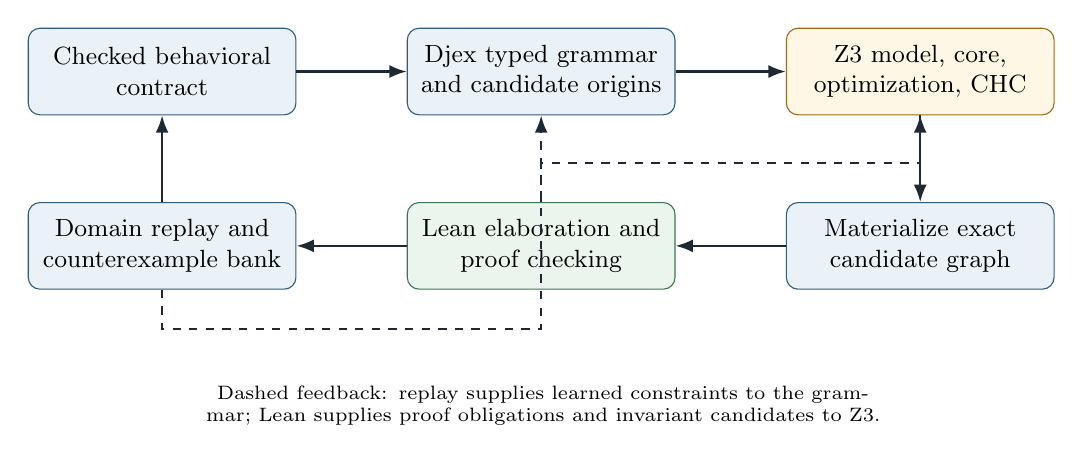
\begin{tikzpicture}[
  node distance=11mm and 14mm,
  box/.style={draw=accent,rounded corners=1.5mm,fill=accentlight,minimum width=34mm,minimum height=11mm,align=center,font=\small},
  trust/.style={draw=greenline,rounded corners=1.5mm,fill=greenbox,minimum width=34mm,minimum height=11mm,align=center,font=\small},
  solver/.style={draw=amberline,rounded corners=1.5mm,fill=amberbox,minimum width=34mm,minimum height=11mm,align=center,font=\small},
  arr/.style={-{Latex[length=2.2mm]},thick,draw=ink}
]
\node[box] (contract) {Checked behavioral\\contract};
\node[box,right=of contract] (grammar) {Djex typed grammar\\and candidate origins};
\node[solver,right=of grammar] (z3) {Z3 model, core,\\optimization, CHC};
\node[box,below=of z3] (materialize) {Materialize exact\\candidate graph};
\node[trust,left=of materialize] (lean) {Lean elaboration and\\proof checking};
\node[box,left=of lean] (replay) {Domain replay and\\counterexample bank};

\draw[arr] (contract) -- (grammar);
\draw[arr] (grammar) -- (z3);
\draw[arr] (z3) -- (materialize);
\draw[arr] (materialize) -- (lean);
\draw[arr] (lean) -- (replay);
\draw[arr] (replay) -- (contract);
\draw[arr,dashed] (replay.south) -- ++(0,-5mm) -| (grammar.south);
\draw[arr,dashed] (lean.north) -- ++(0,5mm) -| (z3.south);
\node[below=11mm of lean,font=\scriptsize,align=center,text width=112mm] {
  Dashed feedback: replay supplies learned constraints to the grammar; Lean supplies proof obligations and invariant candidates to Z3.
};
\end{tikzpicture}
\caption{The proposed synthesis loop and ownership boundaries.}
\label{fig:ownership-loop}
\end{figure}

\Djex should never ask Z3 to return an untyped string. It should give Z3 either (a) a counterexample formula for an exact candidate, (b) finite selector variables over a type-correct grammar, (c) a sound summary of all completions of a partial state, or (d) a CHC system whose relational meaning is separately defined. Z3 returns a model, core, objective value, or invariant candidate. Djex reifies finite choices and preserves exact identities. Lean checks the resulting term and, when requested, the behavioral theorem.

\section{Generalizing the existing behavioral envelope}

\Djex already has a generic \code{BehavioralProblem} and associated-observation layer. The best extension is not to replace it with a broad type class immediately, but to add a closed existential package around domain-specific checked values.

\begin{lstlisting}[language=HaskellX,caption={Sketch of a first-class behavioral-domain package.},label={lst:domain-package}]
data BehavioralDomainId = BehavioralDomainId
  { domainName    :: Name
  , domainVersion :: Natural
  }

data SomeBehavioralDomain source candidate =
  forall d. SomeBehavioralDomain
    { domainId              :: BehavioralDomainId
    , domainSourceAdmission :: Limits -> source
                             -> Either DomainSourceError (Source d)
    , domainSealSession     :: Inventory -> Source d
                             -> Either (SessionError d) (Session d)
    , domainSealCandidate   :: Session d -> VerifiedOrigin candidate
                             -> Either (CandidateError d) (Problem d)
    , domainLowerQuery      :: Problem d
                             -> Either (LoweringError d) (Query d)
    , domainReplayModel     :: Problem d -> ModelInput d
                             -> Either (ReplayError d) (ReplayResult d)
    , domainProofObligation :: Problem d
                             -> Either (ProofError d) LeanObligation
    }
\end{lstlisting}

The existential type keeps each domain's source, session, problem, query, model and evidence types nominally distinct while allowing generic orchestration. A Haskell type class can still implement the dictionary internally, but a first-class record has practical advantages:

\begin{itemize}[leftmargin=2em]
\item domain selection can be decoded from a versioned contract without an open-world orphan-instance mechanism;
\item the exact function bundle can enter a domain implementation fingerprint;
\item experimental domains can remain package-private while sharing the orchestration layer;
\item no generic code needs a type-family branch for every domain;
\item tests can inject deliberately restricted domains without constructing a global instance.
\end{itemize}

The record must not expose constructors for checked values. Existing domain modules should continue to own the only sealers and evidence producers.

\section{Seven semantic artifacts}

Each domain should expose the following conceptual pipeline, even when several artifacts are represented by one opaque value.

\begin{enumerate}[leftmargin=2em]
\item \textbf{Source contract.} Passive, bounded syntax supplied by Leant or an embedding client. It can name source declarations but carries no authority that the names resolve.
\item \textbf{Checked contract.} The source syntax after type, role, nominal-family, provider-law, and normalization checks against an exact inventory.
\item \textbf{Checked session.} The inventory, semantic model, provider assumptions, interpretation policy, resolver authority, and domain version sealed atomically.
\item \textbf{Candidate problem.} One exact verified typed candidate associated with one checked contract and session, including all actual provider laws used by symbolic interpretation.
\item \textbf{Solver query.} A bounded typed plan and canonical bytes derived from the problem. The query is reproducible and cannot outlive its problem association.
\item \textbf{Observation.} Raw status and bounded artifact associated with the query and solver execution identity. It has no semantic authority.
\item \textbf{Evidence or proof.} A replayed counterexample, bounded validation receipt, domain-established receipt, or Lean-checked theorem. Each records the exact authority it does and does not provide.
\end{enumerate}

This is deliberately compatible with the current Length flow. The generic layer should first wrap Length without changing its bytes or error precedence, then host new domains.

\section{A separate selection boundary}

The existing post-verification boundary proves that a behavioral assessor supplied a permutation of the exact input receipts. Hard constraints need a different nominal result:

\begin{lstlisting}[language=HaskellX,caption={An additive boundary for behaviorally selected candidates.},label={lst:selection-boundary}]
data BehavioralSelectionPolicy
  = PreserveOnUnknown
  | RejectOnUnknownExplicitly
  | RequireLeanProof

data BehavioralSelectionBatch candidate = BehavioralSelectionBatch
  { selectedCandidates :: [Verified candidate]
  , rejectedCandidates :: [BehavioralRejection candidate]
  , undecidedCandidates :: [BehavioralUnknown candidate]
  }

withBehavioralSelectionInput
  :: VerificationBatch candidate
  -> (forall epoch. BehavioralSelectionInput epoch candidate -> result)
  -> result

sealBehavioralSelectionBatch
  :: SelectionLimits
  -> BehavioralSelectionPolicy
  -> BehavioralSelectionInput epoch candidate
  -> [SelectionDecision epoch candidate]
  -> Either BehavioralSelectionError (BehavioralSelectionBatch candidate)
\end{lstlisting}

A decision handle must be minted from the exact verification batch, just like the current post-verification candidate handle. The seal checks one and only one decision per input occurrence, forbids foreign epochs, and validates that a rejection contains an evidence receipt whose candidate fingerprint matches that occurrence. Unknown policy is explicit. This boundary must not be represented as a permutation with missing elements, because omission would otherwise lose the proof of why a candidate disappeared.

\section{Generic orchestration, domain-specific semantics}

The following facilities are good candidates for shared infrastructure:

\begin{itemize}[leftmargin=2em]
\item contract acquisition limits, file admission, version tags and canonical fingerprints;
\item solver process admission, executable identity, deadlines, cancellation, causal stream framing and bounded response parsing;
\item typed \QFLIA, bit-vector, datatype, array, sequence, optimization and fixedpoint command syntax;
\item raw observation association and artifact limits;
\item counterexample-bank ownership, LRU policy, candidate replay scheduling and result statistics;
\item sketch selector allocation, model decoding, exact-model blocking and assumption-literal tracking;
\item cache identities, execution profiles, diagnostics and observability metrics.
\end{itemize}

The following must remain domain-specific:

\begin{itemize}[leftmargin=2em]
\item which source types and term-graph forms are modeled;
\item the meaning of opaque values, functions, effects, constructors and recursion;
\item provider-law vocabulary and admissibility;
\item normalization, exactness and approximation direction;
\item conversion from a candidate graph to symbolic semantics;
\item model-input decoding and independent replay;
\item what constitutes a complete bounded validator;
\item the Lean proposition and proof skeleton emitted for positive authority.
\end{itemize}

\begin{caution}
A generic SMT expression type should not become a generic semantic value. Sharing the typed syntax of Z3 theories is useful. Sharing the interpretation of a list, state transition, partial function, or recursive call without an explicit domain is not.
\end{caution}

\section{Architecture layers and dependency direction}

A practical module decomposition is shown in \cref{fig:layers}.

\begin{figure}[htbp]
\centering
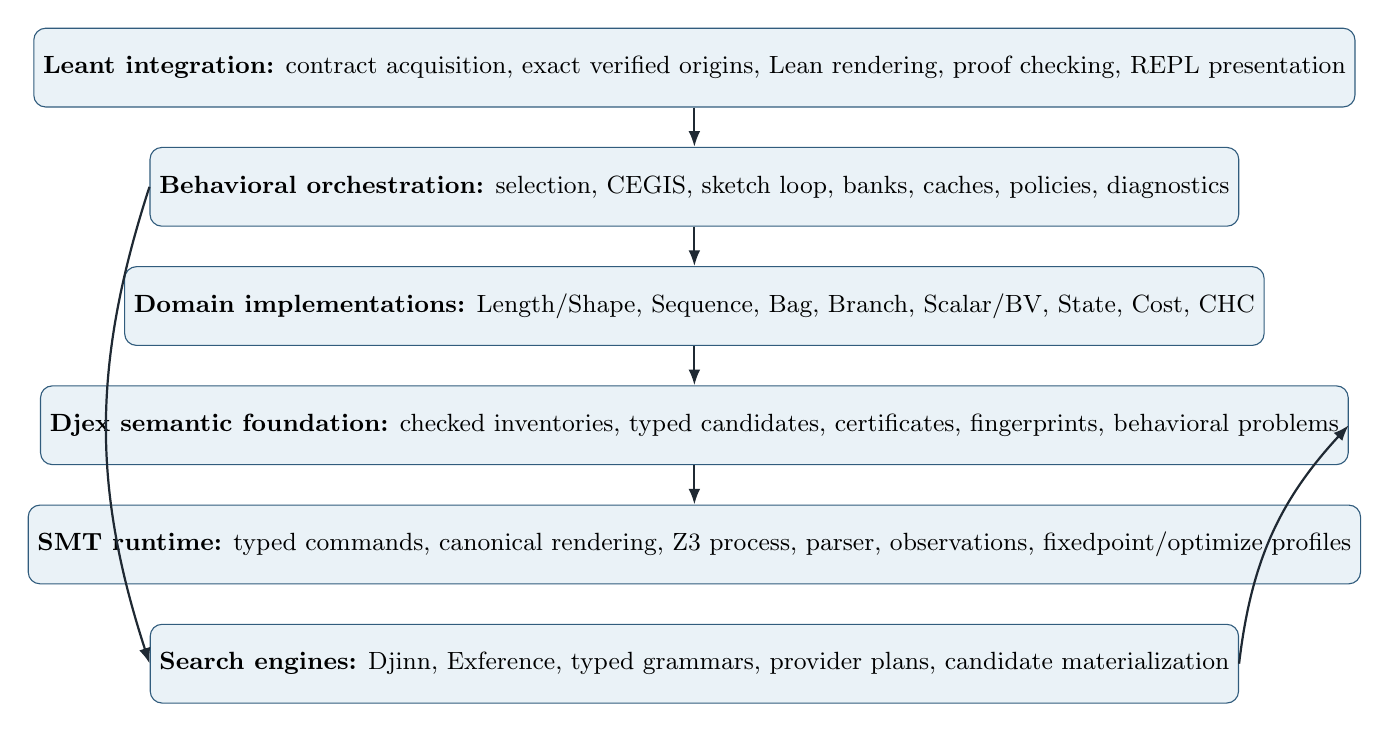
\begin{tikzpicture}[
 layer/.style={draw=accent,fill=accentlight,rounded corners=1.5mm,minimum width=132mm,minimum height=10mm,align=center,font=\small},
 arrow/.style={-{Latex[length=2mm]},draw=ink,thick},
 node distance=5mm
]
\node[layer] (leant) {\textbf{Leant integration:} contract acquisition, exact verified origins, Lean rendering, proof checking, REPL presentation};
\node[layer,below=of leant] (orch) {\textbf{Behavioral orchestration:} selection, CEGIS, sketch loop, banks, caches, policies, diagnostics};
\node[layer,below=of orch] (domains) {\textbf{Domain implementations:} Length/Shape, Sequence, Bag, Branch, Scalar/BV, State, Cost, CHC};
\node[layer,below=of domains] (semantic) {\textbf{Djex semantic foundation:} checked inventories, typed candidates, certificates, fingerprints, behavioral problems};
\node[layer,below=of semantic] (smt) {\textbf{SMT runtime:} typed commands, canonical rendering, Z3 process, parser, observations, fixedpoint/optimize profiles};
\node[layer,below=of smt] (engines) {\textbf{Search engines:} Djinn, Exference, typed grammars, provider plans, candidate materialization};
\draw[arrow] (leant) -- (orch);
\draw[arrow] (orch) -- (domains);
\draw[arrow] (domains) -- (semantic);
\draw[arrow] (semantic) -- (smt);
\draw[arrow,bend right=18] (orch.west) to (engines.west);
\draw[arrow,bend left=18] (engines.east) to (semantic.east);
\end{tikzpicture}
\caption{Recommended layers. Arrows indicate use of checked lower-level capabilities, not transfer of semantic authority.}
\label{fig:layers}
\end{figure}

The search engines should not depend directly on Z3 process code. They depend on an orchestration callback which can answer questions such as ``does this sample reject the candidate?'', ``give me a finite sketch model'', or ``is this prefix provably completion-infeasible?'' The domain and SMT layers implement those answers.


\chapter{Behavioral contract language}
\label{chap:contracts}

\section{Why a contract language is needed}

A command-line flag such as ``preserve length'' is enough for one demonstration but not for a synthesis system. The contract must state at least:

\begin{itemize}[leftmargin=2em]
\item the exact target and its source-ordered argument roles;
\item the semantic domain and its version;
\item preconditions and postconditions;
\item which observations of inputs and results are legal;
\item any explicit examples or forbidden examples;
\item exact source identities of modeled datatypes and providers;
\item assumed provider transfer laws and their required class obligations;
\item whether recursion, case analysis, partiality, overflow, or effects are modeled;
\item the requested positive-proof policy and unknown policy;
\item search preferences which are not hard behavioral requirements.
\end{itemize}

The language should be declarative and solver-neutral. A source file describes the intended behavior. It does not contain SMT-LIB snippets, Z3 parameters, graph identifiers, private Djex names, or proof receipts.

\section{A versioned outer envelope}
\label{sec:contract-envelope}

A proposed outer JSON envelope is shown in \cref{lst:contract-envelope}. JSON is not semantically privileged; it is merely practical for the existing file-acquisition model. The checked in-memory source should be a nominal Haskell type.

\begin{lstlisting}[language=JSONX,caption={Illustrative versioned contract envelope.},label={lst:contract-envelope}]
{
  "format": "leant-behavior-contract",
  "version": 1,
  "domain": { "name": "sequence", "version": 1 },
  "target": {
    "arguments": [
      { "name": "xs", "role": "sequence-input" }
    ],
    "result": { "role": "sequence-result" }
  },
  "requires": [ "true" ],
  "ensures": [
    { "eq": [ { "len": "result" }, { "len": "xs" } ] },
    { "forall-index": {
        "name": "i",
        "range": [0, { "len": "xs" }],
        "body": {
          "eq": [
            { "nth": ["result", "i"] },
            { "nth": ["xs", { "sub": [{"len":"xs"}, 1, "i"] }] }  // xs[len(xs) - 1 - i]
          ]
        }
    }}
  ],
  "provider-laws": [],
  "proof": { "policy": "lean-required" },
  "search": {
    "prefer": ["smaller-term", "fewer-providers"],
    "unknown": "preserve"
  }
}
\end{lstlisting}

The outer version governs field grammar and default behavior. The domain version governs semantic interpretation. Execution profiles and Z3 parameters are separate activated policy files, as they are for Length today; a passive contract must not grant process-launch authority.

A remark on versioning is needed because the current Length entrances deliberately carry none. Since the pinned revision, \Leant's startup and contract-only schemas are each a single versionless document: one \code{format} literal, one \code{rankingDomain} discriminator and one nested object, with no migration decoder and no compatibility promise (\cref{sec:revisions}). That is the right choice for an experimental single-domain entrance: a version field whose only reader is a rejection branch is dead weight. The envelope above asks for versions for a different reason. In a contract language spanning several domains, \code{domain.version} is a \emph{semantic-model identifier}: it enters session and problem fingerprints so that two contracts with identical text under different domain versions are different problems, and it lets a domain change its exactness statement without silently changing the meaning of stored samples, nogoods and proof receipts. The outer \code{version}, by contrast, only matters if more than one field grammar is ever accepted at once. If the project keeps its present policy, the outer version can be dropped in favor of the same format-literal-plus-discriminator shape Length now uses, and the domain version can be folded into the domain identifier; nothing else in this proposal depends on numeric file versions.

\section{Contract core}

The common core should be intentionally small:

\begin{align*}
C &::= \operatorname{requires}(F) \mid \operatorname{ensures}(F)
      \mid \operatorname{example}(E) \mid \operatorname{forbid}(E),\\
F &::= \top \mid \bot \mid F\land F \mid F\lor F \mid \neg F
      \mid F\Rightarrow F \mid R(T_1,\ldots,T_n),\\
T &::= \operatorname{input}(i) \mid \operatorname{result}
      \mid \operatorname{literal} \mid \operatorname{domainTerm}(\ldots).
\end{align*}

Only Boolean connective structure and target references are common. Arithmetic operations, sequence indexing, bag lookup, constructor tags, state projections, costs, and recursive relations belong to a domain or to an explicitly imported observation algebra. The parser may use one JSON AST, but checking must elaborate every domain term into a nominal typed representation.

\section{Target roles and source correspondence}

Current Length contracts already demonstrate why target roles must be explicit. A function argument may be:

\begin{itemize}[leftmargin=2em]
\item an observed value whose model contributes solver variables;
\item an unobserved opaque value which can be forwarded but not inspected;
\item a callback or provider whose applications are modeled relationally;
\item a ghost input used only by a proof contract;
\item a finite-control input such as an enumeration or bit-vector;
\item a state or trace value modeled by a dedicated relation;
\item unsupported, in which case the contract is inapplicable.
\end{itemize}

A role vector is source ordered and arity checked against the exact normalized target. It is not inferred from a type constructor name. Two arguments with the same Lean type may have different roles, and a role may carry additional source identity. For example, a sequence role records the exact modeled family and constructors, while a bit-vector role records width and signedness policy.

\section{Preconditions, partial specifications, and domains of application}

Behavioral synthesis frequently uses partial specifications. A sorting function may be required to behave only when a comparator is a strict order. A division helper may require a nonzero divisor. A parser may be specified only for well-formed input. A contract therefore has a semantic shape
\[
  \forall \vec{x}.\; P(\vec{x}) \Longrightarrow Q(\vec{x}, f(\vec{x})).
\]

The counterexample query is
\[
  P(\vec{x}) \land \neg Q(\vec{x}, f(\vec{x})).
\]

The contract checker must distinguish three questions:

\begin{enumerate}[leftmargin=2em]
\item Is $P$ syntactically and semantically admissible in this domain?
\item Is the application domain nonempty under the selected model?
\item Is $Q$ satisfied for every modeled input in that domain?
\end{enumerate}

A vacuous contract is not the same as a satisfied nonvacuous contract. The existing Length applicable-domain receipts already retain applicable assignment counts; that discipline should become generic. A positive result should report whether nonvacuity was established, assumed, bounded, or unknown.

\section{Examples as first-class constraints}

Examples serve four distinct purposes and should not be conflated.

\begin{description}[leftmargin=2.2em,style=nextline]
\item[Concrete examples.] Exact source values and expected results, executable or reducible by Lean. These can become direct Lean tests and Z3 ground constraints.
\item[Symbolic examples.] A finite set of abstract atoms, lengths, states, or function-table entries. These are CEGIS samples inside a domain, not necessarily source values.
\item[Negative examples.] Inputs on which a particular result or observation is forbidden.
\item[Metamorphic examples.] Relations among multiple calls, such as idempotence $f(f(x))=f(x)$, commutation, monotonicity, or fusion.
\end{description}

Examples should be fingerprinted separately from universal clauses so a CEGIS session can grow the example bank without changing the source contract identity. The complete synthesis-session identity includes the ordered or canonicalized bank.

\section{Provider laws}

A provider law is an explicit assumption describing only the observations a domain needs. It is not a theorem about source evaluation unless separately proved. A general provider-law source might have this shape:

\begin{lstlisting}[language=HaskellX,caption={General shape of an explicit provider law.},label={lst:provider-law}]
data ProviderLawSource d = ProviderLawSource
  { providerSourceName      :: SourceName
  , providerArgumentRoles   :: [ProviderArgumentRole d]
  , providerResultRole      :: ProviderResultRole d
  , providerPrecondition    :: Formula d ProviderVariable
  , providerTransfer        :: Relation d ProviderVariable
  , providerTrustClass      :: ProviderTrustClass
  }

data ProviderTrustClass
  = AssumedUniformLaw
  | AssumedConditionalOnGroundDischarge
  | LeanProvedLaw LeanTheoremName
\end{lstlisting}

The current Length distinction between context-free assumed laws and laws conditional on exact ground class discharge should be retained. A new \code{LeanProvedLaw} class can point to a theorem which Leant checks in the active environment and whose elaborated type is matched against the domain-generated law proposition. The proof theorem then enters the session fingerprint by exact source identity and type, not merely by name.

\section{Hard requirements versus preferences}

Contracts should separate hard requirements from ranking preferences.

\begin{itemize}[leftmargin=2em]
\item \textbf{Hard requirements} enter the counterexample formula and may reject a candidate when a checked counterexample is replayed or a Lean proof obligation fails.
\item \textbf{Soft behavioral preferences} enter a deterministic scoring or Optimize layer but never turn an otherwise valid candidate into a contract violation.
\item \textbf{Syntactic preferences} such as term size, provider count, wildcard use, recursion depth, or source-name ratings are owned by the grammar/search layer.
\item \textbf{Presentation preferences} affect which equivalent spelling is shown and must not alter candidate semantics.
\end{itemize}

A useful rule is that only the hard requirement fingerprint participates in the behavioral problem identity. Soft and syntactic preferences participate in a separate search-policy identity. This permits re-ranking an established candidate set without invalidating behavioral evidence.

\section{Quantification policy}

Unrestricted quantifiers are a recipe for unpredictable SMT behavior and ambiguous exactness. The contract source should expose only domain-owned bounded forms:

\begin{itemize}[leftmargin=2em]
\item finite enumeration over constructor tags or a declared finite type;
\item bounded integer or natural ranges;
\item a sequence index guarded by $0\le i<\operatorname{len}(s)$;
\item one symbolic element atom used for bag-count equality;
\item first-order universal variables in a CHC rule;
\item explicitly finite function tables for examples;
\item no general quantifier over Lean types or higher-order functions.
\end{itemize}

A domain may lower a bounded universal by expansion, an index universal by a fresh counterexample index, or a recursive universal property by CHCs. The checked contract records which transformation was used and whether it is exact.

\section{Exactness descriptors}

Every checked contract should carry a closed exactness descriptor, for example:

\begin{lstlisting}[language=HaskellX,caption={Illustrative exactness vocabulary.},label={lst:exactness}]
data SemanticExactness
  = ExactForModeledSourceFragment
  | ExactWithinFiniteDomain FiniteDomainReceipt
  | OverApproximation CompletionOverApproximationId
  | UnderApproximation WitnessUnderApproximationId
  | ConditionalOnProviderLaws [ProviderLawFingerprint]
  | HeuristicObservationOnly HeuristicReason
\end{lstlisting}

In practice exactness is multidimensional. A candidate may be interpreted exactly for length but only under an assumed provider law; a sequence model may be exact for bounded lists but only a finite-atom abstraction for element equality; a cost model may ignore sharing; a CHC relation may over-approximate evaluation. The internal representation should therefore be a product of independently named claims rather than one enum once multiple domains exist.

\chapter{What Z3 should be used for}
\label{chap:z3-capabilities}

\section{Z3 is a reasoning engine, not the source language}

Z3 can solve rich combinations of first-order theories, expose models and unsat cores, optimize objectives, and run fixedpoint engines. It does not know Lean's binder scoping, implicit arguments, universe constraints, type-class search, source nominal identities, or which generated term graph a rendered expression came from. Those facts belong to \Djex and \Leant.

The productive use of Z3 is therefore to solve a carefully bounded mathematical problem derived from a checked synthesis artifact. The main uses are:

\begin{enumerate}[leftmargin=2em]
\item find an input that violates a candidate's contract;
\item select among finite grammar productions in a typed sketch;
\item prove a finite-choice completion problem infeasible and learn a nogood;
\item optimize a discrete or arithmetic objective after hard constraints hold;
\item infer coefficients, thresholds, branch guards, permutations, or finite tables;
\item solve or refute CHC safety queries for recursive relational semantics;
\item minimize or explain conflicting contract clauses via assumption literals and cores;
\item propose invariants or lemmas for subsequent Lean checking.
\end{enumerate}

\section{Incremental scopes and assumptions}

Z3's push/pop scopes and check-with-assumptions API are directly useful for CEGIS. A synthesis session has a stable base:

\begin{itemize}[leftmargin=2em]
\item declarations for grammar selectors and semantic variables;
\item well-formedness constraints for the sketch;
\item stable provider and datatype axioms admitted by the domain;
\item accumulated sample constraints.
\end{itemize}

Each candidate check adds a temporary goal or a set of active production assumptions. The session can then pop to the stable base without reconstructing every declaration. Assumption literals are preferable when the system needs an unsat core or wants to retract a subset of choices without changing declarations.

The current live Length protocol deliberately resets and serializes query transactions under a strong causal owner. A generic incremental sketch protocol should be a new execution profile, not an informal extension of the Length check/value state machine. Its fingerprint must include scope discipline, assumption order, model requests, core settings, objective priority, and all Z3 parameters.

\section{Models and counterexamples}

A satisfiable counterexample query is the most dependable and useful Z3 result, provided the model is treated as untrusted input:

\begin{enumerate}[leftmargin=2em]
\item decode only the exact requested symbols under explicit byte, node, numeral and collection limits;
\item reject missing, duplicate, ill-sorted, noncanonical or out-of-range values;
\item map solver integers back to naturals, indices, tags, finite atoms, or bit-vectors through a checked domain decoder;
\item replay the exact candidate problem independently;
\item require the precondition to hold and the postcondition to fail in replay;
\item bind the receipt to the exact problem and query fingerprints;
\item only then add the sample to a counterexample bank or reject a candidate.
\end{enumerate}

The existing Length stack already follows this pattern. Every future domain should reuse the generic parser and association machinery but implement its own model decoder and replay.

\section{Unsatisfiable cores}

Z3 can extract cores from tracked assertions or assumptions, although a returned core is not guaranteed minimal \cite{z3-cores}. There are four valuable uses.

\subsection{Contract diagnostics}

Track each hard clause, provider assumption, finite-domain axiom, and target-role constraint with a stable literal. If the contract is inconsistent before any candidate is considered, a core identifies a bounded subset responsible for the contradiction. Leant can report source spans and offer a deterministic deletion-based minimization pass under a separate budget.

\subsection{Grammar nogoods}

When a sketch is infeasible under a set of production choices, a core over choice assumptions yields a learned clause:
\[
  \neg(a_{i_1}\land\cdots\land a_{i_k}).
\]
This nogood can be attached to the exact grammar fingerprint and reused while the sample bank only grows. It must not be reused after changing provider inventory, semantic domain, production meaning, or candidate-size bounds.

\subsection{Explanation of impossible combinations}

A user may request mutually incompatible properties, such as ``reverse'' and ``preserve every index'' for lists of length greater than one. A core can identify the conflicting clauses and a domain can ask Z3 for a small witness to their incompatibility.

\subsection{Proof search guidance}

When a generated Lean proof obligation is discharged by a tactic such as \code{omega}, the corresponding solver core can help choose which hypotheses to include in the emitted theorem or which invariant clauses are essential. The core is advisory; the final minimized theorem is rechecked by Lean.

\section{Optimization and MaxSMT}

Z3's optimization interface supports integer, real and bit-vector objectives and weighted soft constraints, with lexicographic objectives by default \cite{z3-opt}. It is useful after hard behavior has been encoded. Potential objectives include:

\begin{itemize}[leftmargin=2em]
\item minimize AST node count or weighted source cost;
\item minimize provider calls, case splits, duplicated inputs, or recursive calls;
\item minimize the maximum observed output size or symbolic cost;
\item maximize the number or weight of soft examples satisfied;
\item maximize agreement with a preferred semantic profile;
\item lexicographically minimize branch count, then term size, then provider rating.
\end{itemize}

There are two implementation strategies.

\begin{description}[leftmargin=2.2em,style=nextline]
\item[Native Optimize.] Compact and expressive, especially for soft clauses. The complete objective order and priority mode must be fingerprinted, and result reproducibility should be tested across the pinned Z3 release.
\item[Iterative SAT.] Add a cardinality or arithmetic bound, solve, and tighten it. This is easier to integrate with ordinary assumption cores and often gives clearer deterministic progress. It should be the initial implementation for syntactic size; native Optimize can follow for genuinely multiobjective cases.
\end{description}

Optimization never establishes behavior. It chooses among models satisfying the hard encoding. Every materialized candidate still passes Lean elaboration and behavioral replay/proof.

\section{Algebraic datatypes}

Z3 algebraic datatypes can represent finite syntax trees, lists, trees, tuples and enumerations \cite{z3-datatypes}. They are useful in two different roles.

\begin{enumerate}[leftmargin=2em]
\item \textbf{Object semantics.} A domain may represent a bounded or first-order source datatype directly and define observations such as size or constructor tags.
\item \textbf{Sketch syntax.} A finite grammar can be represented by an AST datatype and constrained by a typing relation.
\end{enumerate}

The second role should be used cautiously. Djex already has a checked typed grammar and exact candidate graph. Re-encoding all typing rules as recursive Z3 predicates duplicates a trusted boundary and complicates rank-N terms. For the first typed-sketch implementation, selector variables over a Djex-prepared DAG are preferable to a free Z3 AST. A datatype AST becomes attractive later for domains with small first-order grammars or when Synthesiz3-style symbolic term construction is evaluated.

\section{Sequences and arrays}

Z3 sequences provide concatenation, length, extraction, indexing and related operations over an arbitrary element sort \cite{z3-sequences}. They can make bounded sequence contracts concise, but two caveats matter:

\begin{itemize}[leftmargin=2em]
\item out-of-bounds \code{seq.nth} is under-specified (the guide says the result is treated as a fresh variable), so every index observation must carry and preserve an explicit bounds guard;
\item solver behavior for quantified sequence properties can be less predictable than a domain-specific array-plus-length encoding.
\end{itemize}

A sequence domain should therefore support at least two lowering profiles:

\begin{description}[leftmargin=2.2em,style=nextline]
\item[Native sequence profile.] Use \code{Seq E}, \code{seq.len}, concatenation and guarded \code{seq.nth}. Suitable for concrete counterexamples and concise exact bounded models.
\item[Array-plus-length profile.] Represent a sequence by $(n,a)$ where $n\in\Nat$ and $a:\mathbb{Z}\to E$, with every read guarded by $0\le i<n$. This profile interacts naturally with Skolem counterexample indices and bag-count abstractions.
\end{description}

The profile is part of the encoding fingerprint. A model decoded under one profile cannot be replayed under the other without a domain-owned conversion.

\section{Bit-vectors}

Bit-vectors are essential for precise synthesis of low-level arithmetic \cite{z3-bitvectors}. They model fixed-width wraparound exactly and distinguish signed from unsigned comparisons through operators. A scalar domain should make width, signedness, shift semantics, division-by-zero policy, and source coercions explicit.

A useful first application is synthesis of branchless or saturating operations over \code{UInt32}/\code{Int32}-like Lean types or custom fixed-width structures. Z3 chooses masks, shifts, constants and conditional forms; Lean re-elaborates the term; a generated bit-vector theorem is checked with \code{bv\_decide} where possible. This is a domain in which solver semantics and Lean proof automation can align particularly well.

\section{Recursive functions versus constrained Horn clauses}

Z3 supports recursive function definitions by iterative unfolding, but the official guide explicitly notes that this is not induction and only decides a limited class \cite{z3-recursive}. Recursive-function unfolding is useful for bounded counterexample generation; it is not the right positive-proof foundation for general recursive synthesized programs.

Spacer, Z3's property-directed fixedpoint engine, accepts Horn clauses over arithmetic and Boolean domains and also works with arrays, algebraic datatypes and bit-vectors \cite{z3-spacer}. It is a better fit for relational semantics of recursive programs:

\begin{align*}
\operatorname{Eval}_f(x,y) &\leftarrow \operatorname{Base}(x,y),\\
\operatorname{Eval}_f(x,y) &\leftarrow \operatorname{Step}(x,x',z),
    \operatorname{Eval}_f(x',y'),\operatorname{Combine}(z,y',y),\\
\operatorname{Bad} &\leftarrow \operatorname{Eval}_f(x,y),P(x),\neg Q(x,y).
\end{align*}

A query for \code{Bad} can find a counterexample or infer an inductive invariant. Even then, the fixedpoint result is a solver observation unless the invariant is translated into a Lean lemma and checked. The proposed CHC path therefore has two outputs: a replayable concrete trace for refutation, or an invariant candidate for proof generation.

\section{Synthesiz3 as an adjacent research direction}

The official Z3 documentation repository contains the artifact of Synthesiz3 \cite{synthesiz3}, published at FMCAD 2025, which encodes synthesis specifications of the shape
\[
  \forall \vec{c}.\;\exists y.\;\forall \vec{u}.\;F(\vec{c},y,\vec{u})
\]
using an extended SMT-LIB command, \code{assert-synth}, together with a \code{:uncomputable} option naming the symbols $\vec{u}$ that may appear in the specification but not in the synthesized term. This work is relevant because it demonstrates synthesis-oriented reasoning on top of Z3, especially when specifications contain symbols that may be used logically but not in the synthesized term.

For \Leant/\Djex it should be treated as a research backend, not the first production dependency. The typed-sketch selector encoding proposed here is smaller, uses the existing Z3 process protocol, and keeps term grammar ownership in Djex. A later experimental backend can translate a first-order checked grammar and contract into Synthesiz3's problem shape and compare quality and performance on the same benchmark corpus.

\section{What not to rely on}

\begin{caution}
Do not design the architecture around general quantifier elimination, unrestricted recursive-function proofs, minimal unsat cores, stable model shapes, or an assumption that all solver versions choose the same optimum. These are useful capabilities, not semantic contracts. Every relied-upon profile needs a bounded protocol, explicit parameters, observed capability, and versioned fallback.
\end{caution}


\chapter{Integration strategies: from filtering to synthesis}
\label{chap:strategies}

\section{Level 1: hard post-verification filtering}
\label{sec:hard-filter}

The smallest useful extension is an opt-in hard behavioral filter over already verified candidates. It changes no term grammar and can be implemented first for the existing Length domain.

\subsection{Algorithm}

For each callback-accepted candidate in source order:

\begin{enumerate}[leftmargin=2em]
\item Try the existing exact handoff. An inapplicable candidate receives the configured inapplicability decision: preserve, reject because the contract is mandatory, or place in an undecided tier.
\item Replay every counterexample already in the query-scoped bank. A replayed violation rejects the candidate without opening Z3.
\item Run any complete pure validator enabled by the domain. A replayed violation rejects. A complete positive receipt may accept according to policy.
\item If necessary, lower the exact candidate problem and run the solver.
\item On \texttt{sat}, decode and replay. A reproduced violation rejects the candidate and inserts the input into the bank. A failed replay is an atomic assessment failure, not a non-counterexample.
\item On \texttt{unsat}, either retain the candidate as \emph{solver-undisproved}, request a Lean proof obligation, or accept only under an explicitly configured external-solver trust policy.
\item On \texttt{unknown}, timeout or resource exhaustion, apply the explicit unknown policy. The default is preserve.
\end{enumerate}

\begin{lstlisting}[language=HaskellX,caption={Core hard-filter loop.},label={lst:hard-filter}]
filterCandidate :: Domain d
                -> SelectionPolicy
                -> CounterexampleBank d
                -> VerifiedCandidate
                -> IO (Decision d, CounterexampleBank d)
filterCandidate domain policy bank verified =
  case sealProblem domain verified of
    Left refusal -> pure (onRefusal policy refusal, bank)
    Right problem ->
      case replayBank domain problem bank of
        Violation receipt bank' -> pure (Reject receipt, bank')
        NoViolation bank' ->
          case validatePure domain problem of
            Established receipt -> pure (AcceptEstablished receipt, bank')
            Violation receipt   -> pure (Reject receipt, insert receipt bank')
            Inconclusive        -> runLive domain policy problem bank'
\end{lstlisting}

\subsection{Why this is more than ranking}

A ranking stage can be observationally conservative because the candidate remains visible. A filter changes the result set, so three additional properties are required:

\begin{itemize}[leftmargin=2em]
\item each rejection is associated with the exact verified occurrence and carries replayed evidence;
\item omission and reassociation are checked by a nominal selection seal;
\item unknown and inapplicable results are policy-visible and cannot disappear as ordinary rejection.
\end{itemize}

The first user-visible syntax can be additive:

\begin{lstlisting}[language={},caption={Illustrative Leant command forms.}]
:synth --behavior-contract /abs/preserve-length.json -- TYPE
:synth --behavior-mode filter --behavior-contract /abs/contract.json -- TYPE
:synth --behavior-mode prove --behavior-contract /abs/contract.json -- TYPE
\end{lstlisting}

Existing \code{--length-contract} continues to mean ranking unless an explicit behavior mode is selected, preserving compatibility.

\section{Level 2: counterexample-guided candidate enumeration}
\label{sec:candidate-cegis}

Hard filtering becomes \CEGIS when counterexamples learned from one candidate are used to constrain later candidates. The simplest loop does not ask Z3 to construct terms:

\begin{enumerate}[leftmargin=2em]
\item enumerate the next type-correct candidate from Djinn or Exference;
\item let Lean verify it;
\item replay the current bank;
\item if it survives, ask the domain for a new counterexample;
\item on a replayed counterexample, add the sample and continue enumeration;
\item on positive proof or the configured stopping criterion, return the candidate.
\end{enumerate}

This can eliminate large families cheaply. For \code{List a -> List a}, a single sample of length one eliminates constant-empty and many partial rebuilds; a length-two atom sample separates identity, reverse, head duplication and tail selection; a state-bind sample where the intermediate state differs from the initial state eliminates the classic wrong threading candidate.

\subsection{Bank identity and lifetime}

A counterexample bank is not a bag of integers. It is scoped to:

\[
(\text{domain session},\text{contract},\text{target},\text{provider-law basis},
 \text{model profile}).
\]

The candidate fingerprint is intentionally absent: the bank is meant to cross candidates. Every replay still produces a fresh candidate-specific receipt. A bank entry contains only the minimum domain input necessary for replay, plus provenance and usage statistics. It does not cache a solver verdict, query, candidate, or proof.

Banks can have three lifetimes:

\begin{description}[leftmargin=2.2em,style=nextline]
\item[Batch-local.] Exactly the current Length style, safest and easiest.
\item[Command-local.] Shared across all engine batches and progressive bounds in one \code{:synth} command. Recommended first CEGIS scope.
\item[Persistent.] Saved in a synthesis companion keyed by the exact target/contract/session fingerprint. Useful later, but must survive environment changes only through exact identity checks.
\end{description}

\subsection{Replay ordering}

A good deterministic order is:

\begin{enumerate}[leftmargin=2em]
\item samples which most recently rejected a candidate;
\item samples with the highest historical rejection count;
\item smaller samples under the domain's canonical complexity order;
\item remaining samples in insertion order.
\end{enumerate}

This generalizes the existing small MRU bank while retaining predictable behavior. The bank has independent limits on count, encoded bytes, per-sample width, and cumulative replay work.

\subsection{Semantic signatures}

For each candidate, evaluate the vector of observations on the current bank:
\[
  \sigma_B(c) = \bigl(\operatorname{obs}(c,b_1),\ldots,
                         \operatorname{obs}(c,b_k)\bigr).
\]

This signature is search metadata, not identity. It supports:

\begin{itemize}[leftmargin=2em]
\item suppressing candidates behaviorally identical on all known samples;
\item retaining only the cheapest representative of a sample-equivalence class;
\item selecting a candidate likely to split the largest remaining class;
\item measuring information gain from a new counterexample;
\item interleaving structural novelty with behavioral novelty.
\end{itemize}

A structurally distinct candidate must not lose its typed graph or authority merely because a signature table keeps another representative. The table stores candidate handles, never replaces candidate identity.

\section{Level 3: Z3-completed typed sketches}
\label{sec:typed-sketches}

Typed sketches are the first mode in which Z3 directly participates in term construction, following the broad sketching and syntax-guided-synthesis tradition while retaining Djex ownership of the grammar \cite{sketching,sygus}. The crucial choice is where the grammar comes from.

\begin{recommendation}
Djex should prepare a finite, type-correct selector DAG; Z3 should select alternatives and solve semantic parameters. Do not initially encode the full type system or binder calculus as Z3 datatypes.
\end{recommendation}

\subsection{Sketch representation}

A sketch consists of typed nodes in topological order. Each node has one result type and a finite set of productions already checked by Djex. A production may reference earlier nodes, local binders, globals, constructors, primitive constants, or child holes. For example:

\begin{lstlisting}[language=HaskellX,caption={Conceptual typed selector-DAG representation.},label={lst:sketch-dag}]
data SketchNode local ty = SketchNode
  { sketchNodeId       :: SketchNodeId
  , sketchNodeType     :: ty
  , sketchAlternatives :: NonEmpty (SketchAlternative local ty)
  }

data SketchAlternative local ty
  = UseLocal local
  | UseGlobal CheckedGlobalOccurrence
  | Apply SketchNodeId SketchNodeId
  | Lambda Binder (SketchNodeId)
  | Construct ConstructorId [SketchNodeId]
  | Case SketchNodeId [SketchBranch local]
  | Literal LiteralFamily ParameterSlot
  | Primitive PrimitiveId [SketchNodeId]
\end{lstlisting}

The actual representation should reuse or derive from the checked \code{TermGraph} vocabulary, with occurrence and certificate identities preserved when a selected global is materialized. A sketch alternative is admitted only if every reference, type application, constructor family and provider occurrence has a checked source origin.

\subsection{Selector encoding}

For node $i$ with alternatives $a_{i,1},\ldots,a_{i,m_i}$ introduce selector $s_i$ with
\[
  0 \le s_i < m_i.
\]
Alternatively use one-hot Booleans if unsat cores over individual alternatives are more important. The semantics of node $i$ on sample $b$ is expressed as
\[
  v_{i,b} = \operatorname{ite}(s_i=0,E_{i,0,b},
                \operatorname{ite}(s_i=1,E_{i,1,b},\ldots)).
\]

A shared DAG avoids exponential AST duplication. It also permits Z3 to choose common subexpressions explicitly. Acyclicity is guaranteed by Djex's topological references rather than solved by Z3.

\subsection{Literal and guard synthesis}

Many useful terms require constants or branch thresholds. Parameter slots can have domain-specific finite or arithmetic ranges:

\begin{itemize}[leftmargin=2em]
\item integer coefficients in $[-K,K]$;
\item bit-vector masks of fixed width;
\item small natural literals;
\item constructor tags or tuple projections;
\item a permutation of argument indices;
\item affine branch guards $a_1x_1+\cdots+a_nx_n\le k$;
\item bounded finite lookup tables.
\end{itemize}

These parameters are model values, not source terms, until checked decoding and materialization. The decoder must prove range and representation constraints before creating a literal or primitive application in the candidate graph.

\subsection{Sample constraints}

For every bank sample, assert the hard contract over the root node's symbolic value. Z3 finds selectors and parameters satisfying all current samples. Djex decodes the model into one exact graph. Lean re-elaborates the rendered candidate. The domain then asks for a counterexample to the universal contract.

\begin{lstlisting}[language=HaskellX,caption={Typed-sketch CEGIS loop.},label={lst:sketch-cegis}]
sketchCegis :: SketchSession d -> IO (SketchOutcome d)
sketchCegis session = loop initialBank initialSolver
 where
  loop bank solver = do
    modelResult <- solveSketch solver bank
    case modelResult of
      SketchUnsat core -> pure (NoSketchWithinBounds core)
      SketchUnknown why -> pure (SketchInconclusive why)
      SketchModel raw -> case decodeMaterialize raw of
        Left badModel -> pure (SketchProtocolFailure badModel)
        Right candidate -> do
          verified <- verifyInLean candidate
          case verified of
            Rejected diagnostic ->
              loop bank (blockExactModel raw solver)
            Accepted receipt -> do
              check <- findCounterexample receipt
              case check of
                ReplayedCounterexample cex ->
                  loop (insert cex bank) (assertSample cex solver)
                LeanProofAccepted proof ->
                  pure (FoundCandidate receipt proof)
                NoCounterexampleObserved status ->
                  pure (CandidateSurvives receipt status)
\end{lstlisting}

\subsection{Blocking}

When a model yields a candidate that Lean rejects, block the exact selector/parameter assignment. When it yields a behaviorally failing candidate, the new counterexample usually excludes it automatically, but an exact block is still useful if the sample abstraction does not distinguish the model. Stronger blocks include:

\begin{itemize}[leftmargin=2em]
\item selector-level exact model blocking;
\item structural alpha-equivalence blocking;
\item semantic-signature blocking over the current bank;
\item core-derived nogoods for an infeasible partial assignment;
\item symmetry-breaking constraints for commutative operators or interchangeable holes.
\end{itemize}

Only exact-model blocking is required for correctness. Stronger blocks are optimizations and must not remove a candidate outside the proved equivalence or infeasibility class.

\subsection{Grammar generation strategies}

Three grammar sources should be supported progressively.

\begin{description}[leftmargin=2.2em,style=nextline]
\item[Bounded normal forms.] Generate beta-normal, eta-long structural alternatives for the target: introduce the target's binders, then at each hole offer the locals of the right type, one-layer case splits on locals of a modeled family, constructor applications and tuple formation, up to a node bound. No provider is needed. Best for plumbing terms and logic such as state threading or \code{Option.bind}.
\item[Exference frontier extraction.] Reuse Exference's rated providers and partial search states to create a goal-relevant grammar: the prepared provider occurrences Exference would try at a goal, already type-checked and certificate-associated, become the alternatives of a node of that goal type, and its rating order becomes the alternative order. Best for library composition, where the useful terms are applications of a few loaded functions.
\item[Template families.] Domain-specific skeletons such as folds, maps, affine arithmetic, bit tricks, case splits, or state-threading forms, with parameter slots where the domain expects constants, coefficients or selectors. Best for deep behavior with a small combinatorial shell, such as saturating arithmetic or a clamp.
\end{description}

A sketch identifies the grammar source and all bounds in its fingerprint. ``No sketch'' means no satisfying term in that finite grammar, not uninhabitation of the type or impossibility of the contract in Lean.

\section{Level 4: solver-guided partial-search pruning}
\label{sec:prefix-pruning}

Waiting for a complete candidate can waste most of the search budget. Partial pruning asks whether any completion of a search state could satisfy the known samples or universal abstraction.

\subsection{Completion summaries}

For each typed hole $h$, a domain computes a relation $S_h$ over the observations any permitted completion may produce. The summary is useful when it is an over-approximation:
\[
  \{\operatorname{obs}(t) \mid t\text{ completes }h\} \subseteq S_h.
\]

Substituting $S_h$ into the partial term yields an over-approximation $S_p$ of all complete candidates extending prefix $p$. If
\[
  S_p \land \text{contract samples}
\]
is unsatisfiable, then no completion satisfies the samples and the prefix may be pruned.

Examples of sound summaries include:

\begin{itemize}[leftmargin=2em]
\item interval or affine bounds on list length;
\item possible constructor-tag sets;
\item finite sets of argument dependencies;
\item bit masks of bits known zero, known one, or unknown;
\item possible state-source identities (initial, intermediate, arbitrary);
\item lower and upper bounds on cost;
\item a regular tree grammar of possible shapes.
\end{itemize}

\subsection{A worked example}

Take the target \code{List a -> List a}, the contract $\operatorname{len}(f(xs))=\operatorname{len}(xs)$, and a bank holding one sample, the empty list ($n=0$). Suppose Exference is at the partial state
\[
  \code{fun xs => List.cons ?h}_1\ \code{?h}_2,
  \qquad \code{?h}_1 : a,\quad \code{?h}_2 : \code{List a}.
\]
The Size/Shape domain knows nothing about what will fill \code{?h}$_2$ except its type, so its summary is the weakest sound statement: the completion has \emph{some} length $t\in\Nat$. Composing that with the exact step case gives the prefix summary $\operatorname{len}(\text{result}) = 1 + t$, and the pruning query on the bank is
\[
  1 + t = 0 \;\land\; t \ge 0,
\]
which is unsatisfiable. Every completion of the prefix returns a nonempty list on the empty input, so the prefix and its whole subtree can be pruned, and the receipt records the summary (``$t\ge 0$ for hole \code{?h}$_2$''), the exact bank identity, and the grammar fingerprint that scoped it.

The polarity rule matters here. Had the domain instead summarized \code{?h}$_2$ by the completions it happened to enumerate first, say ``one of the locals'', giving $\operatorname{len}(\text{result})=1+n$, the query on a bank holding a length-one sample would read $1+1=1$ and would also be unsatisfiable, but that would prune a prefix which the completion \code{?h}$_2 :=$ \code{[]} satisfies on that sample. An under-approximation can report ``here is a completion that works'', never ``no completion works''. The over-approximate summary $t\ge0$ correctly leaves the length-one sample satisfiable ($t=0$).

\subsection{Nominal approximation polarity}

The API should make an accidental direction reversal difficult:

\begin{lstlisting}[language=HaskellX,caption={Nominal distinction between completion approximations.}]
data OverApproximation d prefix
-- constructor private to the domain

data UnderApproximation d prefix
-- constructor private to the domain

pruneFromUnsat
  :: OverApproximation d prefix
  -> UnsatObservation
  -> Either ReplayMismatch (PruningReceipt d prefix)

witnessFromSat
  :: UnderApproximation d prefix
  -> SatObservation
  -> Either ReplayMismatch (CompletionWitness d prefix)
\end{lstlisting}

A generic \code{Approximation} flag is too easy to misuse. Distinct nominal types and distinct query constructors should be used.

\subsection{Assumption-literal learning}

Associate each search decision with an assumption literal. When an over-approximate completion query is unsatisfiable, extract a core and learn a nogood over only the decisions that matter. Exference can use the nogood as a memoized forbidden partial pattern. The receipt is scoped to the exact grammar, sample bank and summary-domain fingerprints.

\subsection{Fairness}

Pruning must not accidentally convert a heuristic search into a false completeness claim. Search status should record:

\begin{itemize}[leftmargin=2em]
\item whether every pruned prefix carried a checked pruning receipt;
\item whether some prefixes were dropped by ordinary queue/resource limits;
\item whether the domain refused summaries for some constructs;
\item whether the sample bank, rather than the universal contract, justified pruning;
\item whether the remaining grammar was explored exhaustively.
\end{itemize}

Only a fully explored finite grammar with checked pruning receipts can produce ``no satisfying sketch within this grammar.'' It still cannot produce a general nonexistence theorem unless the grammar is known complete for the type and contract fragment.

\section{Level 5: recursive synthesis with CHCs}
\label{sec:chc-synthesis}

Recursive synthesis requires separating three tasks:

\begin{enumerate}[leftmargin=2em]
\item choose a recursive program schema;
\item prove or refute its behavioral relation;
\item prove termination in Lean.
\end{enumerate}

Z3/Spacer can assist with the second task. Djex and Lean must own the first and third.

\subsection{Relational encoding}

For a candidate schema, generate a relation \code{Eval} rather than a recursive SMT function. Each constructor case becomes a Horn rule. Provider calls become relations with explicit assumed or proved laws. The bad state is a rule whose body contains the evaluation relation, precondition and negated postcondition.

For list reverse with an accumulator, for example:

\begin{align*}
\operatorname{RevAcc}(\operatorname{nil},a,a) &.\\
\operatorname{RevAcc}(\operatorname{cons}(x,xs),a,r) &\leftarrow
  \operatorname{RevAcc}(xs,\operatorname{cons}(x,a),r).
\end{align*}

A sequence or bag abstraction can replace full element lists when that is the selected domain. Spacer may prove safety by finding an invariant such as
\[
  \operatorname{len}(r)=\operatorname{len}(xs)+\operatorname{len}(a)
\]
or a corresponding bag equation.

\subsection{Invariant extraction and Lean proof}

A solver-produced invariant should be normalized into the domain's proposition language, checked to mention only admitted symbols, and translated to a Lean lemma. Leant then attempts a proof skeleton:

\begin{lstlisting}[language=LeanX,caption={Illustrative generated invariant proof skeleton.}]
theorem revAcc_length_invariant
    (xs acc : List a) :
    (revAcc xs acc).length = xs.length + acc.length := by
  induction xs generalizing acc with
  | nil => simp [revAcc]
  | cons x xs ih =>
      simp [revAcc, ih, Nat.add_assoc, Nat.add_comm, Nat.add_left_comm]
\end{lstlisting}

The exact proof will vary, but the architecture is stable: Spacer proposes a predicate; the domain translates it; Lean proves it; the final candidate theorem uses it. If proof generation fails, the invariant remains advisory and may still guide search.

\subsection{Termination}

CHC safety says nothing by itself about Lean's acceptance of a recursive definition. Candidate materialization must use a structurally recursive schema, a well-founded measure, or an existing recursive provider. Lean's termination checker and any generated \code{termination\_by}/\code{decreasing\_by} proof remain authoritative.

\section{Level 6: specification and law inference}

A later, clearly labeled experimental mode can use Z3 to infer unknown contract parameters or provider summaries:

\begin{itemize}[leftmargin=2em]
\item infer affine length transfer coefficients from examples;
\item infer which input state a candidate uses;
\item infer a branch threshold or bit mask;
\item infer a finite permutation or projection;
\item infer candidate invariants for recursive code;
\item infer a weakest condition within a restricted predicate grammar.
\end{itemize}

These outputs are \emph{proposals}. A provider law becomes usable only after explicit user acceptance or a Lean theorem establishing it. The system must never convert ``fits the current examples'' into an assumed universal law automatically.

\section{Hybrid scheduling}

The modes above should not form one mandatory pipeline. A scheduler can interleave them:

\begin{enumerate}[leftmargin=2em]
\item run cheap sample replay on ordinary Djinn/Exference candidates;
\item periodically ask a typed sketch solver for a model satisfying all samples;
\item when the sketch solver is unsatisfiable, widen grammar bounds or resume ordinary enumeration;
\item use semantic signatures to avoid rechecking redundant candidates;
\item launch expensive universal or CHC checks only for candidates that survive cheap stages;
\item request Lean proof generation only for the best surviving candidates.
\end{enumerate}

Fairness requires explicit lanes and budgets. A fast sketch lane must not starve complete Djinn search in a fragment where a definitive logical result is possible. Conversely, a provider-heavy Exference lane should not consume the whole behavioral budget before the compact sketch lane runs.


\chapter{Behavioral domains}
\label{chap:domains}

\section{Domain 1: generalized size and shape}
\label{sec:domain-size-shape}

The existing Length domain should become the seed of a broader Size/Shape family, not be discarded. Its current implementation already provides exact finite-spine identities, role-aware symbolic inputs, modeled zero/step cases, provider transfers, scalar and pair results, bounded evaluation, QF-LIA lowering, and extensive finite applicable-domain validation.

\subsection{Generalization axes}

A versioned Size/Shape domain can add the following observations while retaining the same trust pattern:

\begin{itemize}[leftmargin=2em]
\item size of arbitrary structurally checked unary recursive families;
\item constructor counts for multi-constructor datatypes;
\item tree height, minimum depth and leaf count;
\item product-field sizes of arbitrary fixed arity;
\item sums and maxima of component sizes;
\item whether a result is empty/nonempty or belongs to a bounded shape class;
\item affine and piecewise-affine provider transfers;
\item exact one-layer case behavior for each modeled constructor.
\end{itemize}

For a datatype
\[
D\;\alpha = C_1(\vec{p}_1,\vec{r}_1)\mid\cdots\mid C_k(\vec{p}_k,\vec{r}_k),
\]
a size model declares one equation per constructor, for example
\[
\operatorname{size}(C_j(\vec{p},r_1,\ldots,r_m))
 = c_j + \sum_i w_{j,i}\operatorname{size}(r_i).
\]
The source family and recursive fields must come from an exact checked schema. The caller may choose coefficients only within a domain version that defines their meaning.

\subsection{Shape abstractions}

Full algebraic values are often unnecessary. A finite shape abstraction can use:

\begin{itemize}[leftmargin=2em]
\item root constructor tag;
\item bounded depth-$d$ constructor tree;
\item size interval;
\item constructor-count vector;
\item nullary/non-nullary and singleton/multiple classifications.
\end{itemize}

These abstractions are useful for early pruning. They are exact only within the declared observation. They do not imply element preservation or source evaluation behavior.

\subsection{Recommended first extension}

Add an exact \emph{constructor-tag plus size} domain for \code{Option}, \code{Except}, user enums and list-like families. This unlocks precise \code{Option.bind}, error propagation, nonempty preservation, and branch behavior with minimal new theory beyond integers and finite tags.

\section{Domain 2: sequences and indexed behavior}
\label{sec:domain-sequence}

A sequence domain observes order, not merely size. Its core checked value is an abstract finite sequence over an element sort $E$. For polymorphic Lean elements, $E$ is an uninterpreted sort whose equality means only equality in the model.

\subsection{Core observations}

\begin{align*}
\operatorname{len}(s) &\in \Nat,\\
\operatorname{nth}(s,i) &\in E \quad\text{under }0\le i<\operatorname{len}(s),\\
\operatorname{concat}(s,t) &\in \operatorname{Seq}(E),\\
\operatorname{slice}(s,o,n) &\in \operatorname{Seq}(E),\\
\operatorname{reverse}(s) &\in \operatorname{Seq}(E).
\end{align*}

A first implementation does not need a primitive reverse. It can express the law with a fresh counterexample index:
\[
0\le i<n \land \operatorname{nth}(r,i)\ne
\operatorname{nth}(x,n-1-i).
\]

\subsection{Candidate interpretation}

The symbolic interpreter can model:

\begin{itemize}[leftmargin=2em]
\item spine zero and step constructors as empty and singleton-prepend;
\item exact zero/step case analysis;
\item tuples and lets;
\item providers with explicit sequence transfers such as identity, append, reverse, map and filter abstractions;
\item opaque elements which may be forwarded and compared for modeled equality but not called or inspected;
\item index-safe primitives admitted by a domain-specific provider law.
\end{itemize}

Map requires a relational element provider. Rather than interpret an arbitrary Lean function, assign an uninterpreted unary symbol $F:E\to E'$ to the exact callback argument and state the result law pointwise. The model assumes totality because SMT uninterpreted functions are total; the contract descriptor must record that this is a mathematical extensional model, not a claim about source strictness, effects or nontermination.

\subsection{Bounded versus unbounded modes}

\begin{description}[leftmargin=2.2em,style=nextline]
\item[Finite-spine bounded mode.] Enumerate lengths up to $N$ and finite atoms up to $A$. Exact for that finite abstraction; suitable for fast counterexamples and exhaustive bounded receipts.
\item[Index-counterexample mode.] Use unbounded length and one or more symbolic indices. Exact for quantifier-free index laws after guarded Skolemization when candidate semantics is expressible in the chosen theory.
\item[CHC mode.] Use relational list semantics and inductive invariants for recursive providers or candidates. Appropriate for unbounded proof attempts.
\end{description}

\section{Domain 3: bags, multisets, and permutations}
\label{sec:domain-bag}

Length preservation cannot distinguish \code{id}, \code{reverse}, rotations, duplicating one element while deleting another, or many other transformations. Bag equality adds element multiplicity while ignoring order.

\subsection{Finite-atom encoding}

For a bounded atom set $A=\{a_1,\ldots,a_k\}$, represent a bag by counts
\[
  \operatorname{count}_s(a_j)\in\Nat.
\]
Bag equality is a conjunction over all atoms. This is exact for the finite-atom abstraction and works well in CEGIS: Z3 can invent an atom assignment that exposes duplication or loss.

\subsection{Symbolic-witness encoding}

For generic elements, introduce one symbolic witness $e:E$ and ask for
\[
  \operatorname{count}_{r}(e)\ne\operatorname{count}_{x}(e).
\]
This transforms a universal bag-equality law into an existential counterexample witness. Candidate interpretation must provide a count transfer for constructors and providers. The encoding is exact for the modeled count semantics if recursive count equations are handled exactly or relationally.

\subsection{Array encoding}

A bag can be represented as an SMT array $E\to\mathbb{Z}$ constrained nonnegative at observed indices. Constructor insertion becomes a store/update. This is concise for finite candidate expressions, but universal nonnegativity and extensional equality require care. Prefer pointwise witness queries and domain replay rather than asking for full array models.

\subsection{Combined specifications}

Useful contracts layer observations:

\begin{itemize}[leftmargin=2em]
\item \textbf{Permutation:} length equality plus bag equality.
\item \textbf{Stable filter:} result is an order-preserving subsequence plus a predicate law.
\item \textbf{Partition:} bag union equals input, output bags are disjoint by predicate, and each output preserves relative order.
\item \textbf{Deduplication:} result is a subsequence, contains each observed atom at most once, and preserves membership.
\end{itemize}

Each layer should produce a separate subreceipt so diagnostics can say whether a candidate preserved size but violated multiplicity or order.

\section{Domain 4: constructor and branch behavior}
\label{sec:domain-branch}

Many important functions are characterized by their constructor cases. Examples include \code{Option.bind}, \code{Except.map}, defaulting, error propagation, and one-layer destructors.

A branch domain observes:

\begin{itemize}[leftmargin=2em]
\item input constructor tags;
\item output constructor tag;
\item selected payload provenance;
\item which callback/provider occurrence was invoked;
\item whether a callback is unused, called once, or may be called multiple times in the modeled graph;
\item branch-specific value relations.
\end{itemize}

\subsection{Finite tag encoding}

Constructor tags form a finite datatype or integer enumeration. A candidate graph with exact case authority can be interpreted as an if-then-else over tags. Payloads are opaque tokens with stable provenance classes. This allows a contract such as:

\[
\begin{array}{rcl}
\operatorname{bind}(\operatorname{none},f) &=& \operatorname{none},\\
\operatorname{bind}(\operatorname{some}(x),f) &=& f(x).
\end{array}
\]

The second equation is relational: the result must equal the modeled application of the exact callback token to the exact payload token. No source evaluation is performed.

\subsection{Call traces}

A finite call-trace abstraction can record a bounded sequence of provider-call events:
\[
  \operatorname{Call}(p,\vec{v}),\quad \operatorname{Return}(p,r).
\]
It can distinguish short-circuiting, callback duplication, ignored arguments and state-threading. The trace is a mathematical graph-evaluation trace, not a claim about Lean's runtime evaluation order unless a domain version defines one for a restricted pure fragment.

\section{Domain 5: scalar arithmetic}
\label{sec:domain-scalar}

Scalar arithmetic is a natural domain for precise synthesis because Z3 can solve equations over integer, rational, nonlinear and bit-vector terms, while Lean has strong proof tactics for many resulting obligations.

\subsection{Natural and integer profiles}

A QF-LIA profile supports:

\begin{itemize}[leftmargin=2em]
\item affine expressions and inequalities;
\item min, max, monus, positive-literal quotient and modulo through checked lowering;
\item piecewise-affine branches;
\item bounded coefficient synthesis;
\item monotonicity or range counterexamples with two calls;
\item lexicographic cost objectives.
\end{itemize}

The current Length implementation already contains a sophisticated natural arithmetic normalizer and applicable-domain machinery. That code should be factored into a reusable arithmetic observation library only where its semantics is genuinely domain-independent.

\subsection{Nonlinear arithmetic}

Nonlinear integer arithmetic can be useful for polynomial templates, but solver completeness and performance are less predictable. Treat it as a separate profile with strict time and degree bounds. A successful model can synthesize coefficients; an unsat result remains heuristic unless a Lean tactic proves the resulting polynomial theorem.

\subsection{Relational properties}

Properties such as monotonicity, injectivity on a bounded range, Lipschitz bounds or idempotence require multiple symbolic calls:

\begin{align*}
 x_1\le x_2 &\Longrightarrow f(x_1)\le f(x_2),\\
 f(x_1)=f(x_2) &\Longrightarrow x_1=x_2,\\
 f(f(x)) &= f(x).
\end{align*}

A candidate interpreter must either duplicate a pure symbolic evaluation with shared provider symbols or refuse providers/effects that make such extensional duplication unsound under the model.

\section{Domain 6: machine arithmetic and bit-vectors}
\label{sec:domain-bitvector}

A bit-vector domain models exact fixed-width values. It is suitable for:

\begin{itemize}[leftmargin=2em]
\item constant and mask synthesis;
\item branchless min/max/absolute-value idioms;
\item saturating add/subtract;
\item population count or parity templates;
\item byte packing and unpacking;
\item sign extension, truncation and rotate/shift operations;
\item low-level range checks and overflow detection.
\end{itemize}

The grammar should consist of a curated safe primitive set with exact Lean renderers. Z3 chooses operator selectors, constants and wiring. The target proof proposition is translated to Lean bit-vector or fixed-width arithmetic and checked by \code{bv\_decide}, normalization, or a library theorem. Undefined or source-dependent operations are excluded unless their Lean semantics is modeled exactly.

\section{Domain 7: state transitions and relational effects}
\label{sec:domain-state}

The motivating state-bind type
\[
(S\to A\times S)\to(A\to S\to B\times S)\to S\to B\times S
\]
has multiple inhabitants. A correct bind must satisfy
\[
\begin{aligned}
(a,s_1)&=f(s_0),\\
(b,s_2)&=g(a,s_1),\\
\operatorname{bind}(f,g,s_0)&=(b,s_2).
\end{aligned}
\]

This is expressible without knowing the internal meanings of $S$, $A$ or $B$. Model them as uninterpreted sorts and $f$, $g$ as uninterpreted total functions into tuple datatypes. Congruence is enough to distinguish passing $s_1$ from passing $s_0$.

\subsection{Provenance relational semantics}

A lightweight alternative to full uninterpreted functions tracks symbolic provenance terms:

\begin{align*}
F_s &= \pi_2(F(s_0)),\\
F_a &= \pi_1(F(s_0)),\\
G_b &= \pi_1(G(F_a,F_s)),\\
G_s &= \pi_2(G(F_a,F_s)).
\end{align*}

The candidate result is compared structurally to $(G_b,G_s)$. A wrong candidate using $G(F_a,s_0)$ differs in the free term algebra and is refuted by congruence unless the model happens to equate the states; Z3 can choose a separating interpretation.

\subsection{General state contracts}

The same domain can describe:

\begin{itemize}[leftmargin=2em]
\item reader environment threading;
\item writer log concatenation;
\item lens get-put and put-get laws;
\item transaction state invariants;
\item parser state/position progression;
\item finite protocol transitions;
\item relational refinement between two state implementations.
\end{itemize}

Effects are modeled only as explicit mathematical state. IO, exceptions, nondeterminism or nontermination require separate domains or explicit monadic providers with laws.

\section{Domain 8: cost and resource behavior}
\label{sec:domain-cost}

A cost domain attaches a symbolic nonnegative cost to term-graph operations and provider calls. It can express:

\begin{itemize}[leftmargin=2em]
\item number of provider calls or constructor allocations;
\item maximum recursion depth under a recurrence;
\item affine time or memory estimates;
\item upper bounds conditional on input sizes;
\item multiobjective preferences after semantic correctness.
\end{itemize}

Cost semantics is especially sensitive to sharing and evaluation strategy. The first version should define cost on the \emph{term graph interpretation}, not claim actual Lean runtime cost. Lets may share a node; duplicated applications may count twice; opaque providers use explicit assumed cost transfers. The contract displays this model prominently.

A proof-grade cost theorem is possible only when the source program is instrumented or related to a formal cost semantics in Lean. Until then, cost remains a search objective or modeled contract.

\section{Domain 9: recursive relational behavior}
\label{sec:domain-recursive}

This domain packages the CHC path from \cref{sec:chc-synthesis}. It should be introduced only after nonrecursive exact domains are stable. Its checked contract identifies:

\begin{itemize}[leftmargin=2em]
\item the exact recursive candidate schema and calls;
\item a relational abstraction of values;
\item base and step rules;
\item admitted provider relations;
\item candidate termination authority in Lean;
\item a bad-state predicate;
\item an invariant grammar acceptable for Lean translation.
\end{itemize}

The main outputs are concrete counterexample traces or candidate invariants. A fixedpoint ``safe'' status by itself remains an observation. A Lean proof of the invariant and theorem upgrades the result.

\section{Domain 10: higher-order finite observations}
\label{sec:domain-higher-order}

Arbitrary higher-order extensional equality is out of scope, but useful finite observations are possible. A function argument can be modeled by:

\begin{itemize}[leftmargin=2em]
\item an uninterpreted function over first-order modeled sorts;
\item a finite table on the current sample atoms;
\item a symbolic callback with exact call/return events;
\item an algebraic law supplied as an explicit provider contract;
\item a universally quantified first-order relation in CHC mode.
\end{itemize}

The chosen observation class must be explicit. For example, treating a callback as an SMT uninterpreted function assumes extensionality, totality and purity in the mathematical model. This is excellent for distinguishing argument wiring; it is not a theorem about evaluation effects.

\begin{recommendation}
Prioritize domains in this order: generalized size/tag, state/provenance, sequence/index, scalar/bit-vector, bag/permutation, then recursive CHC. This order maximizes reuse of the existing graph interpreter and QF-LIA/Z3 stack while delivering behavior that types alone fail to express.
\end{recommendation}

\chapter{Worked synthesis scenarios}
\label{chap:examples}

\section{From \texttt{List a -> List a} to exact intent}
\label{sec:example-list}

The type
\[
  \forall \alpha.\;\operatorname{List}\alpha\to\operatorname{List}\alpha
\]
admits many programs. Behavioral constraints can be layered to move from a broad family to a precise implementation.

\subsection{Layer 1: length preservation}

\[
  \forall xs.\;\operatorname{len}(f(xs))=\operatorname{len}(xs).
\]

This rejects every candidate whose output length can differ from the input length: constant empty or singleton results, functions that drop or duplicate elements without compensation, and truncations. It retains identity, reverse, rotations, arbitrary permutations, element replacement, and duplicate/delete combinations whose net length change is zero.

The existing Length domain can already rank candidates by counterexamples to this law. The first proposed hard-filter milestone can reject replayed violators.

\subsection{Layer 2: bag preservation}

\[
  \forall xs,e.\;\operatorname{count}(f(xs),e)=\operatorname{count}(xs,e).
\]

Together with length, this characterizes permutation behavior in the mathematical list model. It rejects element replacement and duplicate/delete compensation. It retains identity, reverse and permutations.

\subsection{Layer 3a: identity}

\[
  \forall xs,i.\;0\le i<\operatorname{len}(xs)
  \Longrightarrow f(xs)[i]=xs[i].
\]

This pins the result pointwise. In a parametric pure total setting it is equivalent to list equality, but the domain should prove or assume only the selected sequence semantics.

\subsection{Layer 3b: reverse}

\[
  \forall xs,i.\;0\le i<n
  \Longrightarrow f(xs)[i]=xs[n-1-i],\qquad n=\operatorname{len}(xs).
\]

A sketch grammar can include:

\begin{itemize}[leftmargin=2em]
\item \code{xs};
\item \code{List.reverse xs};
\item \code{List.map g xs};
\item \code{List.foldr step init xs};
\item one-layer cases and constructors;
\item selected loaded providers with explicit sequence laws.
\end{itemize}

On two finite-atom samples, Z3 may immediately choose \code{List.reverse}. The provider occurrence is materialized with its exact scheme and Lean source name. Lean elaborates the term. A proof-mode request then emits the theorem

\begin{lstlisting}[language=LeanX,caption={Desired proof artifact for a reverse candidate.}]
def it1 {a : Type u} : List a -> List a := List.reverse

theorem it1_contract {a : Type u} (xs : List a) :
    it1 xs = xs.reverse := by
  rfl
\end{lstlisting}

If the candidate is a hand-built fold, the theorem requires list induction; the proof generator can use the provider laws and standard simp lemmas.

\section{Correct state threading}
\label{sec:example-state}

Consider the type:

\begin{lstlisting}[language=LeanX]
(S -> Prod A S) -> (A -> S -> Prod B S) -> S -> Prod B S
\end{lstlisting}

A type-directed synthesizer may produce both:

\begin{lstlisting}[language=LeanX,caption={Correct and incorrect inhabitants of the same state-bind type.}]
-- correct
fun f g s0 =>
  match f s0 with
  | (a, s1) => g a s1

-- wrong: reuses the initial state
fun f g s0 =>
  match f s0 with
  | (a, _) => g a s0
\end{lstlisting}

\subsection{SMT model}

Declare uninterpreted sorts $S,A,B$ and functions
\[
F:S\to A\times S,\qquad G:A\times S\to B\times S.
\]
For symbolic $s_0$, define
\[
 a=\pi_1(F(s_0)),\quad s_1=\pi_2(F(s_0)),\quad
 expected=G(a,s_1).
\]
The wrong candidate denotes $G(a,s_0)$. Ask whether they differ. Z3 can choose a model with $s_0\ne s_1$ and distinguish the two applications by congruence.

\subsection{Replay}

The replay need not produce actual Lean values of arbitrary $S,A,B$. It re-evaluates the exact symbolic term graph in the same free algebra and checks that the candidate result term differs from the contract term under the decoded finite model. The receipt says ``relational state-threading counterexample in the uninterpreted total-function model,'' not ``concrete runtime counterexample.''

\subsection{Lean proof}

A proof-grade contract can quantify over the actual functions and state and define the expected expression in Lean:

\begin{lstlisting}[language=LeanX,caption={Lean theorem shape for state bind.}]
theorem bind_contract
    (bind : (S -> Prod A S) -> (A -> S -> Prod B S) -> S -> Prod B S)
    (hbind : bind = fun f g s0 =>
      match f s0 with | (a, s1) => g a s1) :
    forall f g s0,
      bind f g s0 =
        (match f s0 with | (a, s1) => g a s1) := by
  intro f g s0
  simp [hbind]
\end{lstlisting}

For a synthesized closed term, Leant substitutes the candidate directly and asks \code{rfl}, \code{simp}, or structural tactics to prove the equation.

\section{Option bind}
\label{sec:example-option}

The type
\[
\forall \alpha\,\beta.\;\operatorname{Option}\alpha\to
(\alpha\to\operatorname{Option}\beta)\to\operatorname{Option}\beta
\]
admits the always-\code{none} function. A branch contract specifies:

\begin{align*}
 f(\operatorname{none},k) &= \operatorname{none},\\
 f(\operatorname{some}(x),k) &= k(x).
\end{align*}

The branch domain uses exact constructor tags and payload provenance. A two-sample sketch problem suffices: one \code{none} sample and one \code{some} sample with a callback table that returns a distinguishable token. The correct case expression survives; the constant \code{none} candidate fails the second sample.

The generated proof is direct case analysis:

\begin{lstlisting}[language=LeanX]
theorem optionBind_contract {a b : Type}
    (x : Option a) (k : a -> Option b) :
    it1 x k = Option.bind x k := by
  cases x <;> rfl
\end{lstlisting}

This is an ideal early vertical slice because it exercises exact constructor cases, callback provenance, sketch selectors, Lean materialization and a simple proof artifact without recursive semantics.

\section{Partition into two lists}
\label{sec:example-partition}

Suppose the target is
\[
(\alpha\to\Bool)\to\operatorname{List}\alpha\to
\operatorname{List}\alpha\times\operatorname{List}\alpha.
\]
A useful behavioral contract states:

\begin{enumerate}[leftmargin=2em]
\item every input occurrence appears in exactly one output bag;
\item every element in the first output satisfies the predicate;
\item every element in the second does not;
\item relative order within each output is preserved;
\item output lengths sum to input length.
\end{enumerate}

The current Length pair domain already models two list-spine fields and can express the length sum. A staged extension can add:

\begin{itemize}[leftmargin=2em]
\item a predicate callback represented as an uninterpreted Boolean function;
\item bag counts parameterized by a symbolic element;
\item a stable-subsequence sequence relation;
\item a recursive fold/filter provider law or CHC relation.
\end{itemize}

This example is valuable as an integration benchmark because each domain catches a different defect: dropping elements, duplicating elements, swapping sides, ignoring the predicate, and reversing one side.

\section{Map with a behavioral callback law}
\label{sec:example-map}

For
\[
(\alpha\to\beta)\to\operatorname{List}\alpha\to\operatorname{List}\beta,
\]
the contract is
\begin{align*}
\operatorname{len}(r)&=\operatorname{len}(xs),\\
r[i]&=g(xs[i])\quad(0\le i<\operatorname{len}(xs)).
\end{align*}

The callback $g$ becomes an uninterpreted function $G:E_\alpha\to E_\beta$. A candidate which ignores $g$ can build a \code{List b} only from constructors and providers that need no $\beta$ value, such as the constant empty list, and the length clause already rejects those; a candidate which applies $g$ to the wrong element, applies it twice to one element, or reverses the list is distinguishable by a symbolic index and atom model.

When the selected candidate is \code{List.map}, Leant can generate a proof by reflexivity after unfolding the alias. A fold-based implementation may require induction and standard list lemmas. Provider laws can be either assumed or linked to Lean theorems.

\section{Saturating addition over fixed-width words}
\label{sec:example-saturating}

A bit-vector sketch can synthesize a saturating unsigned addition:
\[
\operatorname{satAdd}(x,y)=
\begin{cases}
2^w-1,&x+y\text{ overflows},\\
x+y,&\text{otherwise}.
\end{cases}
\]

A grammar may include addition, unsigned comparison, conditional, all-ones, zero, and selected masks. Z3 solves selector and constant variables exactly in \QFBV. The model is decoded into a typed primitive graph, rendered to Lean, and checked. The universal theorem is then discharged by \code{bv\_decide} or a bit-vector normalization tactic.

This scenario demonstrates the full positive path with no provider-law assumptions and a decidable finite domain.

\section{Tree transformation with a size invariant}
\label{sec:example-tree}

For a recursive tree function, a size contract may be simple even when value semantics is not:
\[
  \operatorname{size}(f(t))=\operatorname{size}(t).
\]

A finite-depth shape model can quickly reject candidates that drop or duplicate subtrees. A CHC relation can then reason about unbounded size. Spacer may propose an affine invariant. Leant translates it into an induction lemma over the exact user-declared family and asks Lean to prove it. The candidate is accepted as proof-grade only after that theorem succeeds and the recursive definition passes termination checking.


\chapter{Concrete API and codebase changes}
\label{chap:api}

\section{Preserve the current ownership seams}

The proposed implementation should preserve the following existing seams exactly where possible:

\begin{itemize}[leftmargin=2em]
\item \code{Verified candidate} remains the callback-acceptance receipt. It is not upgraded in place into behavioral evidence.
\item \code{ExactTypedVariantOrigin} remains the Leant-owned route from accepted text to exact typed candidate and semantic provenance.
\item \code{TypedCandidate} remains the Djex-owned carrier for compatibility output, checked graph availability, and certificate association.
\item \code{BehavioralProblem} remains the generic association of domain, inventory, encoding, candidate and problem fingerprints.
\item raw \code{SolverObservation} and \code{BehavioralObservation} remain honest report vocabularies with no automatic evidence conversion.
\item the current Length session/contract/problem/query/evaluator/live stack remains the reference implementation and compatibility adapter.
\item process launch authority remains separate from passive contracts.
\end{itemize}

Generalization should occur by adding orchestration and domain packages around these values, not by making their constructors public or weakening their nominal roles.

\section{Proposed Djex modules}

\cref{tab:djex-modules} lists an additive module plan. Names are illustrative but follow the current repository's organization.

\begin{longtable}{@{}L{0.43\textwidth}L{0.51\textwidth}@{}}
\caption{Proposed Djex module additions.}\label{tab:djex-modules}\\
\toprule
Module & Responsibility \\
\midrule
\endfirsthead
\toprule
Module & Responsibility \\
\midrule
\endhead
\bottomrule
\endfoot
\path{Language.Haskell.Synthesis.Semantic.Domain} & First-class closed domain dictionary, domain identifiers, exactness claims, common refusal classes and existential packaging. \\
\path{Language.Haskell.Synthesis.Semantic.Contract} & Solver-neutral outer contract envelope, target-role correspondence, hard/soft separation, clause/source-span identities and canonical contract fingerprints. \\
\path{Language.Haskell.Synthesis.Semantic.Selection} & Nominal post-verification selection input, exact decision seal, rejection/unknown/established batches and evidence association checks. \\
\path{Language.Haskell.Synthesis.Semantic.Counterexample} & Domain-neutral bank owner, bounded insertion/LRU policy, sample provenance, replay scheduling, bank fingerprints and statistics. \\
\path{Language.Haskell.Synthesis.Semantic.CEGIS} & Candidate-level CEGIS state machine, progressive bounds, stopping criteria and lane scheduling. \\
\path{Language.Haskell.Synthesis.Semantic.Sketch} & Checked typed selector DAG, grammar identities, selector/literal slots, materialization, exact model blocking and sketch result envelope. \\
\path{Language.Haskell.Synthesis.Semantic.Sketch.SMTLib} & Generic finite selector and sample-constraint lowering over domain-provided symbolic node semantics. \\
\path{Language.Haskell.Synthesis.Semantic.Approximation} & Nominal over-/under-approximation wrappers, prefix-query association, pruning receipts and core-derived nogoods. \\
\path{Language.Haskell.Synthesis.Semantic.ProofObligation} & Backend-neutral proof proposition, named hypotheses, provider-law assumptions and exact candidate/contract association. \\
\path{Language.Haskell.Synthesis.Semantic.SizeShape} & Generalized Length-compatible size/tag domain; initially an adapter over current Length scalar and pair implementations. \\
\path{Language.Haskell.Synthesis.Semantic.Sequence} & Sequence roles, expressions, formulas, interpreter, finite/index profiles, model decoder and replay. \\
\path{Language.Haskell.Synthesis.Semantic.Bag} & Count/bag expressions, finite-atom and symbolic-witness profiles, replay and combined permutation receipts. \\
\path{Language.Haskell.Synthesis.Semantic.Branch} & Constructor-tag, payload-provenance and bounded callback-trace semantics. \\
\path{Language.Haskell.Synthesis.Semantic.Scalar} & General scalar expression/formula foundation and proof-obligation lowering; reuse of exact arithmetic normalizers where legitimate. \\
\path{Language.Haskell.Synthesis.Semantic.BitVector} & Width-indexed operations, fixed-width model decoding, primitive grammar and Lean proposition projection. \\
\path{Language.Haskell.Synthesis.Semantic.State} & Uninterpreted relational state/callback semantics and provenance replay. \\
\path{Language.Haskell.Synthesis.Semantic.Cost} & Explicit graph-cost model, provider cost transfers and optimization objectives. \\
\path{Language.Haskell.Synthesis.Semantic.CHC} & Checked relational rules, bad-state query, invariant vocabulary and exact association with a recursive candidate schema. \\
\path{Language.Haskell.Synthesis.Internal.SMTLib.Optimize} & Typed optimization commands/objectives and bounded response handling, independent of ordinary solver authority. \\
\path{Language.Haskell.Synthesis.Internal.SMTLib.Fixedpoint} & Typed relation/rule/query commands, fixedpoint response framing and invariant/certificate artifact bounds. \\
\path{Language.Haskell.Synthesis.Internal.SMTLib.Theory.*} & Reusable typed syntax for arrays, datatypes, sequences and bit-vectors, without domain interpretation. \\
\end{longtable}

The curated \path{Language.Haskell.Djex} facade should initially expose only orchestration types needed by Leant and the mature Size/Shape adapter. Experimental domains can remain focused module imports until their contracts stabilize.

\section{Proposed Leant modules}

\begin{longtable}{@{}L{0.43\textwidth}L{0.51\textwidth}@{}}
\caption{Proposed Leant module additions.}\label{tab:leant-modules}\\
\toprule
Module & Responsibility \\
\midrule
\endfirsthead
\toprule
Module & Responsibility \\
\midrule
\endhead
\bottomrule
\endfoot
\code{Leant.Synth.Behavior.Contract} & Lean-facing passive contract source, exact source names, target role sources and domain selection. \\
\code{Leant.Synth.Behavior.Contract.File} & Versioned JSON grammar and bounded decoder; adapters for existing Length contract files. \\
\code{Leant.Synth.Behavior.Configuration} & Activated execution/search/proof policy, solver pinning and resource limits. \\
\code{Leant.Synth.Behavior.Handoff} & Generic verified-origin recovery and domain dispatch; preserves Length's exact refusal order through its adapter. \\
\code{Leant.Synth.Behavior.Selection} & Integration of the Djex selection seal with one verification batch. \\
\code{Leant.Synth.Behavior.CEGIS} & Command-local sample bank, engine/sketch scheduling and progressive bound control. \\
\code{Leant.Synth.Behavior.Sketch} & Translation of Lean source inventories and semantic families into Djex sketch grammars; exact rendering/materialization variants. \\
\code{Leant.Synth.Behavior.Proof} & Lean proposition rendering, theorem submission, tactic portfolio, proof receipt and failure diagnostics. \\
\code{Leant.Synth.Behavior.Presentation} & Candidate status, counterexamples, assumptions, proof strength, cores and statistics. \\
\code{Leant.Synth.Behavior.Session} & Snapshot companion data for persistent contracts, samples and proof artifacts under exact fingerprints. \\
\end{longtable}

The existing \code{Leant.Synth.Length.*} hierarchy should not be renamed immediately. \code{Behavior.Handoff} can dispatch the Size/Shape-v1 selection to the current Length handoff. Once the generic orchestration proves stable, internal factoring can remove duplication without changing the public file schemas.

\section{Core types}

\subsection{Behavioral source and activation}

\begin{lstlisting}[language=HaskellX,caption={Proposed passive contract and activated policy split.},label={lst:source-policy}]
data LeanBehaviorContractSource = LeanBehaviorContractSource
  { behaviorContractFormatVersion :: Natural
  , behaviorDomainSource          :: LeanBehaviorDomainSource
  , behaviorTargetSource          :: LeanBehaviorTargetSource
  , behaviorHardClauses           :: [LeanBehaviorClauseSource]
  , behaviorSoftPreferences       :: [LeanBehaviorPreferenceSource]
  , behaviorProviderLawSources    :: [LeanBehaviorProviderLawSource]
  , behaviorProofRequest          :: LeanBehaviorProofRequest
  }

data BehaviorExecutionPolicy = BehaviorExecutionPolicy
  { behaviorUnknownPolicy       :: UnknownPolicy
  , behaviorInapplicablePolicy  :: InapplicablePolicy
  , behaviorSolverProfile       :: SolverExecutionProfile
  , behaviorCegisLimits         :: CegisLimits
  , behaviorSketchLimits        :: Maybe SketchLimits
  , behaviorProofPolicy         :: ProofPolicy
  }
\end{lstlisting}

The source is passive and can be parsed without opening a process. The activated policy carries execution authority and is created only through the same explicit admission/pinning pattern as current Length ranking.

\subsection{Candidate decisions}

\begin{lstlisting}[language=HaskellX,caption={Candidate decision vocabulary.},label={lst:decision}]
data BehavioralDecision d candidate
  = CandidateRejected
      (Verified candidate)
      (CounterexampleEvidence d)
  | CandidateEstablished
      (Verified candidate)
      (EstablishedEvidence d)
  | CandidateLeanProved
      (Verified candidate)
      LeanProofReceipt
  | CandidateSurvives
      (Verified candidate)
      (PositiveObservation d)
  | CandidateUndecided
      (Verified candidate)
      BehavioralUnknown
  | CandidateInapplicable
      (Verified candidate)
      DomainRefusal
\end{lstlisting}

Constructors should probably remain private, with domain and Lean proof modules producing nominal receipts. The type shown here illustrates the distinctions the public projections must preserve.

\subsection{Counterexample bank}

\begin{lstlisting}[language=HaskellX,caption={Counterexample bank with no cached verdict authority.},label={lst:bank}]
data CounterexampleBank d = CounterexampleBank
  { counterexampleBankSession     :: SessionFingerprint d
  , counterexampleBankContract    :: ContractFingerprint d
  , counterexampleBankModel       :: ModelProfileFingerprint d
  , counterexampleBankEntries     :: Seq (BankEntry d)
  , counterexampleBankStatistics  :: BankStatistics
  }

data BankEntry d = BankEntry
  { bankInput         :: CounterexampleInput d
  , bankOrigin        :: CounterexampleOrigin
  , bankComplexity    :: CounterexampleComplexity d
  , bankUseCount      :: Natural
  , bankRejectCount   :: Natural
  }
\end{lstlisting}

No \code{CandidateFingerprint}, \code{SolverStatus}, query bytes, receipt or proof is stored in an entry. Replaying against a candidate mints fresh association.

\subsection{Sketch authority}

\begin{lstlisting}[language=HaskellX,caption={Separation of grammar, solver model and materialized candidate.},label={lst:sketch-authority}]
data CheckedSketchGrammar d local ty
-- opaque; owns exact typed alternatives and source origins

data AssociatedSketchModel d grammar
-- raw model associated with grammar, sample bank and execution profile

data MaterializedSketchCandidate d local ty
-- exact graph plus model/grammar receipt, not yet Lean-verified

materializeSketchModel
  :: CheckedSketchGrammar d local ty
  -> AssociatedSketchModel d grammar
  -> Either SketchModelError (MaterializedSketchCandidate d local ty)
\end{lstlisting}

A model cannot be decoded against a different grammar even if selector names happen to match. Grammar node and alternative coordinates are not durable identities; canonical grammar fingerprints abstract away allocation where possible while preserving semantics and order where it matters.

\section{Refactoring the Length adapter}

The first generic-domain implementation should be an adapter, not a rewrite:

\begin{lstlisting}[language=HaskellX,caption={Conceptual adapter over the current Length implementation.}]
lengthBehaviorDomain :: SomeBehavioralDomain
lengthBehaviorDomain = SomeBehavioralDomain
  { domainId = BehavioralDomainId "finite-spine-length" 1
  , domainSourceAdmission = decodeExistingLeanLengthSelection
  , domainSealSession = sealViaCurrentLengthSession
  , domainSealCandidate = prepareViaCurrentLengthHandoff
  , domainLowerQuery = sealViaCurrentLengthAdapter
  , domainReplayModel = replayViaCurrentLengthProblem
  , domainProofObligation = renderLengthLeanObligation
  }
\end{lstlisting}

The adapter should preserve existing scalar/product nominal distinctions, the exact configuration schemas, fingerprint bytes, executable policy, refusal constructors and ranking behavior. New selection/CEGIS modes consume the adapter through new code paths; ordinary ranking remains unchanged.

\section{Term-graph requirements for sketches and domains}

The current semantic foundation already identifies a future limitation: Djinn candidates do not yet retain the same typed graph authority as Exference because historical LJT sidecars erased source names, provider rewrites, assumption identity and nominal type structure. This has direct consequences:

\begin{itemize}[leftmargin=2em]
\item exact candidate-level behavior can initially remain Exference-only where a domain requires a graph;
\item Djinn candidates can still participate in Lean proof-mode behavior by rendering the accepted term and generating a theorem, because Lean is the proof authority;
\item a future Djinn graph lowerer must be built from checked proof construction before final cleanup/rendering, not reconstructed from text;
\item sketch generation should reuse the shared checked grammar and Exference-origin path first;
\item combined-engine exact-text deduplication must retain variant-scoped Exference authority exactly as current Length handoff does.
\end{itemize}

\begin{recommendation}
Do not block the behavioral roadmap on a complete Djinn typed-graph migration. Implement Exference-backed exact semantics and Lean-proof fallback first, while designing the shared graph lowerer as a parallel correctness project.
\end{recommendation}

\section{Provider certificates in sketch materialization}

A sketch alternative that uses a provider must preserve the same information as a directly generated Exference occurrence:

\begin{itemize}[leftmargin=2em]
\item exact source owner scheme;
\item source-ordered explicit type selections;
\item activated constraints;
\item occurrence-specific certificate row and slot handles;
\item final visible-application node;
\item exact ground-discharge receipts where required;
\item renderer metadata for Lean named/positional type arguments.
\end{itemize}

The safest design is for the sketch grammar to contain \emph{prepared provider occurrences}, not provider names plus free type variables. Materialization then selects an already checked occurrence plan and builds the same certificate-associated graph form Exference would have emitted. Z3 never chooses a source type by inventing a string; it chooses among bounded checked selections or among a parameter domain whose decoded type is rechecked before graph construction.

\section{SMT protocol families}

The current Length live protocol is intentionally narrow. New uses should have distinct nominal protocol identities.

\begin{description}[leftmargin=2.2em,style=nextline]
\item[Counterexample protocol.] Reset, assert exact bad-state formula, check, request only required input values, replay. This is the current pattern.
\item[Incremental sketch protocol.] Declare stable selectors, assert grammar and accumulated samples, use assumptions or push/pop, request selector/parameter values, optionally request a core.
\item[Optimization protocol.] Declare hard sketch constraints and ordered objectives, check, request model and objective values. Separate response types from ordinary SAT.
\item[Fixedpoint protocol.] Declare relations/variables/rules, query bad state, retrieve bounded answer or invariant text under a domain-specific decoder.
\end{description}

They may share the same domain-neutral process owner, lexical parser and causal driver, but should not share one phase-state type with optional commands. A state machine that can ask for an unsat core after a model-producing query or issue Optimize commands to a fixedpoint context is too permissive.

\section{Solver-neutral query IR}

A layered query IR avoids hand-built SMT strings:

\begin{enumerate}[leftmargin=2em]
\item theory terms: Bool, Int/Real, bit-vector, array, datatype and sequence;
\item typed commands: declarations, assertions, assumptions, objectives, fixedpoint rules;
\item domain plan: exact symbol roles and formula components;
\item canonical renderer and structural fingerprint projection;
\item bounded expected-response schema.
\end{enumerate}

The renderer and fingerprint projection must consume the same typed plan. A query fingerprint should not be computed from rendered bytes alone; structural fields catch accidental renderer equivalences and keep names/roles explicit. Conversely, the exact rendered bytes should enter the execution observation so replay can detect protocol drift.

\section{Caching}

There are several distinct caches with different safety rules.

\begin{longtable}{@{}L{0.20\textwidth}L{0.32\textwidth}L{0.39\textwidth}@{}}
\caption{Cache classes and required identities.}\label{tab:caches}\\
\toprule
Cache & Key & Safe payload \\
\midrule
\endfirsthead
\toprule
Cache & Key & Safe payload \\
\midrule
\endhead
\bottomrule
\endfoot
Preparation cache & Lean environment generation, target, provider-discovery policy & Prepared semantic origin/inventory projections under existing generation rules. \\
Contract cache & Inventory, domain source, limits, domain version & Checked passive contract/session only; no process handle. \\
Candidate-problem cache & Session, contract, exact typed candidate, interpretation policy & Opaque checked problem; invalidated by any graph/provider/certificate change. \\
Counterexample bank & Session, contract, target, model profile & Domain input vectors and provenance only. \\
Query cache & Problem, lowering profile and limits & Canonical query plan/bytes; no solver status. \\
Observation cache & Query, solver executable/version/profile, exact parameters & Raw associated observation; must still replay before evidence use. \\
Evidence cache & Exact problem plus domain verifier version and limits & Opaque replay/validation receipt, if its replay authority and limits are immutable. \\
Lean proof cache & Exact theorem text/environment fingerprint/backend version & Accepted elaboration receipt or saved theorem declaration; normal session replay rules apply. \\
Nogood cache & Grammar, bank, domain summary, assumptions & Checked grammar-choice nogoods only. \\
\end{longtable}

Raw solver \texttt{sat} should not be cached as a counterexample. Cache the bounded observation if useful, then replay it for the exact problem. A persistent counterexample bank stores decoded inputs only after successful replay at origin, but each later candidate still replays them freshly.

\chapter{Lean proof-producing integration}
\label{chap:proofs}

\section{Why proof production changes the value proposition}

Counterexample guidance can produce excellent programs, but the user eventually wants to know whether the behavior was established. The strongest integration is to bind each synthesized definition to a generated theorem:

\begin{lstlisting}[language=LeanX,caption={Candidate plus behavioral theorem as the final artifact.}]
def it1 : TARGET := CANDIDATE

theorem it1_behavior : CONTRACT_PROP it1 := by
  -- generated and Lean-checked proof
\end{lstlisting}

This design lets Z3 remain an untrusted accelerator. A solver model finds bugs. An invariant or core guides proof construction. The Lean backend checks the final proposition in the exact environment, with actual types, universes, instances and definitions.

\section{Proof-obligation generation}

A domain-generated obligation contains:

\begin{itemize}[leftmargin=2em]
\item exact target type and candidate binding;
\item source-order binders for contract inputs;
\item precondition and postcondition rendered in Lean;
\item explicit provider-law hypotheses or references to checked theorems;
\item model exactness hypotheses if the domain is conditional;
\item any auxiliary invariant statements;
\item suggested imports and tactics;
\item exact association to the candidate and contract fingerprints.
\end{itemize}

The proposition renderer is domain-specific. It must not simply pretty-print the SMT formula: natural monus, sequence indexing, bit-vector operations, constructor tests and provider relations must map to actual Lean definitions whose semantics matches the domain.

\section{Proof tactic portfolio}

A bounded proof portfolio can be selected by the obligation profile.

\begin{longtable}{@{}L{0.24\textwidth}L{0.28\textwidth}L{0.39\textwidth}@{}}
\caption{Suggested Lean proof strategies by domain.}\label{tab:proof-tactics}\\
\toprule
Obligation profile & Initial tactics & Notes \\
\midrule
\endfirsthead
\toprule
Obligation profile & Initial tactics & Notes \\
\midrule
\endhead
\bottomrule
\endfoot
Definitional equality & \code{rfl}, \code{simp} & Best for selected providers, projections and direct case expressions. \\
Propositional finite cases & \code{decide}, cases, simp & Constructor/tag contracts and finite enums. \\
Presburger arithmetic & \code{omega}, simp (\code{norm\_num} where Mathlib is imported) & Natural/integer affine obligations, including monus, \code{min}/\code{max} and quotient/modulo by literals, which \code{omega} handles natively; \code{if-then-else} must be split first. Unfold only named candidate/provider definitions. \\
Bit-vector equality & \code{bv\_decide}, simp & Requires exact width/source semantics; \code{bv\_decide} lives in core Lean but needs \code{import Std.Tactic.BVDecide} in the active environment. \\
List/tree structural property & induction, simp\_all, omega & Z3/Spacer may propose the invariant or generalized induction hypothesis. \\
Equality using library provider & simp [candidate, provider theorem] & Prefer checked source theorem references over re-proving provider internals. \\
Finite bounded domain & \code{native\_decide} or explicit enumeration & Appropriate only when the theorem itself states the bound/finite type. \\
Relational state wiring & rfl, simp, cases on tuple result & Uninterpreted-function counterexamples guide choice; proof is usually definitional. \\
CHC invariant & induction/well-founded induction + arithmetic tactics & Solver invariant is translated and checked before use. \\
\end{longtable}

All tactics named in the table except \code{norm\_num} are part of core Lean at the referenced toolchain; \code{grind}, also in core, is a reasonable later addition to the arithmetic and structural rows once its behavior on generated obligations has been measured. The proof runner should retain Leant's present crash/restart and exact environment replay behavior. Proof-state suggestions are not authority; only successful declaration submission produces a receipt.

\section{Reconstructing QF-LIA unsatisfiability in Lean}

For an exact scalar candidate problem, the Z3 counterexample formula has the form
\[
  \exists \vec{x}\in\Nat.\;P(\vec{x})\land\neg Q(\vec{x}).
\]
An unsat result corresponds to
\[
  \forall \vec{x}\in\Nat.\;P(\vec{x})\to Q(\vec{x}).
\]

Rather than import a Z3 proof, generate this universal proposition using the same normalized expression tree and ask Lean's \code{omega} to prove it. This yields a practical proof-producing bridge for the current Length arithmetic fragment. The key requirements are:

\begin{itemize}[leftmargin=2em]
\item one shared normalized expression algebra with separately verified Lean and SMT renderers;
\item differential tests comparing bounded evaluation of both projections;
\item a pre-processing step for the one construct \code{omega} does not handle: it decides linear arithmetic over \code{Nat}/\code{Int} including natural subtraction, \code{min}/\code{max} and division or modulo by numeric literals, but it does not case-split \code{if-then-else}, so the $\operatorname{caseLen}$ conditional must be split first (\code{split <;> omega}) or rendered as two equations;
\item provider transfer laws as theorem hypotheses or checked theorem references;
\item exact candidate interpretation theorem connecting the synthesized term to the arithmetic result expression.
\end{itemize}

The last item is the difficult one. The current symbolic interpreter derives an arithmetic expression from a typed graph, but a Lean theorem must connect that graph interpretation to the actual term. For simple constructor/provider fragments, Leant can generate a structural proof by unfolding the candidate and provider-law theorems. This should be the first proof-producing subset.

A complete small instance shows the two halves. For the candidate
\begin{lstlisting}[language=LeanX]
def it1 {a : Type u} : List a -> List a :=
  fun xs => match xs with
    | [] => []
    | x :: rest => x :: rest
\end{lstlisting}
the Length interpreter derives $r(n)=\operatorname{caseLen}(n,0,(n\mathbin{\dot{-}}1)+1)$, and Z3 reports \texttt{unsat} for $r(n)\ne n$. The arithmetic half of the reconstructed theorem is the universal form of that query, and the connecting half relates the term to its interpretation:
\begin{lstlisting}[language=LeanX,caption={Reconstructed obligation for a length-preserving one-layer case.}]
theorem it1_len_arith (n : Nat) :
    (if n = 0 then 0 else (n - 1) + 1) = n := by
  split <;> omega

theorem it1_len {a : Type u} (xs : List a) :
    (it1 xs).length =
      (if xs.length = 0 then 0 else (xs.length - 1) + 1) := by
  cases xs <;> simp [it1]

theorem it1_contract {a : Type u} (xs : List a) :
    (it1 xs).length = xs.length := by
  rw [it1_len]; exact it1_len_arith _
\end{lstlisting}
The first theorem is what \Zthree's \texttt{unsat} corresponds to; the second is what the symbolic interpreter silently assumed; only the third is the user-facing claim, and it is accepted by Lean, not by the solver.

\section{Provider assumptions as hypotheses}

Suppose the candidate uses \code{List.reverse} under an assumed length law. A proof-grade theorem should either:

\begin{enumerate}[leftmargin=2em]
\item reference a checked theorem such as \code{List.length\_reverse}; or
\item expose the provider law as a theorem hypothesis in a generic obligation.
\end{enumerate}

It must not present a conclusion as unconditional merely because the SMT session assumed the transfer. A useful presentation is:

\begin{lstlisting}[language=LeanX,caption={Making a provider law explicit when no source theorem is linked.}]
theorem it1_contract
    (h_reverse : forall (xs : List a),
      (List.reverse xs).length = xs.length)
    (xs : List a) :
    (it1 xs).length = xs.length := by
  simp [it1, h_reverse]
\end{lstlisting}

In ordinary Lean environments the system should prefer linking the actual library theorem. Explicit hypotheses remain useful for opaque project providers.

\section{Reusing Leant's existing proof machinery}
\label{sec:proof-reuse}

\Leant already contains most of the runtime this chapter needs, and the proposal should be read as a client of it rather than a second implementation. Its \code{:prove} mode drives the backend's proof-state protocol: every line is a tactic run against an immutable proof state, goals reprint after each step, and a Lean-verified suggestion is computed by actually running candidate tactics against that state. The probes are ordered from quick finishers (\code{rfl}, \code{assumption}, \code{contradiction}, \code{trivial}, \code{decide}, \code{omega}) through goal-shaped structural steps (\code{intro}, \code{cases}/\code{obtain}, \code{left}/\code{right}, \code{induction}) to chained forms such as \code{induction l <;> simp\_all [myLen] <;> omega}, which is how a one-line suggestion can already be a finished induction. \code{:auto} tries an ordered finisher list (\code{rfl}, \code{trivial}, \code{decide}, \code{simp}, \code{omega}, \code{exact?}, and \code{aesop} where the project imports it), and \code{:qed NAME} turns the accumulated script into a theorem saved in the session. Proof-state identifiers belong to one backend process; if that process stops, \Leant leaves prove mode and prints the script instead of submitting a stale identifier after restart.

Four consequences follow for behavioral proof mode:

\begin{enumerate}[leftmargin=2em]
\item the portfolio in \cref{tab:proof-tactics} is a domain-indexed refinement of \code{:auto}'s list and should run through the same proof-state protocol, inheriting its per-tactic timeouts and its rule that only an accepted tactic counts;
\item an obligation the portfolio does not close is not a dead end: \code{:behavior-proof} can open the generated statement in \code{:prove}, so the user finishes it interactively with the same suggestions, and \code{:qed} produces the theorem;
\item \code{:qed}'s save path is the natural producer of the \code{LeanProofReceipt} of \cref{sec:proof-receipts}, because it already threads the environment generation and snapshot identity that the receipt must record;
\item the one-process rule for proof-state identifiers is exactly the crash/restart discipline a proof receipt must inherit; a receipt minted under a backend that has since restarted is replayed or invalidated by the normal environment logic, never trusted by name.
\end{enumerate}

Suggestions remain advisory, as they are today. Only successful declaration submission produces a receipt.

\section{Proof receipts and theorem identity}
\label{sec:proof-receipts}

A \code{LeanProofReceipt} should retain:

\begin{itemize}[leftmargin=2em]
\item backend environment generation or snapshot identity;
\item exact theorem source submitted;
\item exact candidate definition name and body identity;
\item elaborated theorem declaration name and type;
\item active imports and options relevant to elaboration;
\item candidate/contract/problem fingerprints;
\item provider theorem identities;
\item whether the theorem was saved into the session, a transient example, or a snapshot companion.
\end{itemize}

A theorem name alone is not enough because it may be shadowed or redefined after reset. The normal Leant environment-threading and snapshot logic should own durability.

\section{Proof-mode user experience}

A successful command might present:

\begin{lstlisting}[language={},caption={Illustrative proof-grade synthesis output.}]
  it1  fun xs => xs.reverse
       behavior: proved in Lean
       theorem: it1_behavior
       contract: sequence/reverse-v1
       assumptions: none
       counterexamples examined: 3
       sketch models blocked: 1
\end{lstlisting}

A non-proof positive result is labeled honestly:

\begin{lstlisting}[language={}]
  it1  fun xs => xs.reverse
       behavior: no counterexample found
       solver: unsat for exact QF_LIA length projection
       Lean proof: not requested
       additional sequence clauses: validated on 12 symbolic samples only
\end{lstlisting}

This granularity is preferable to a single green check mark.

\section{Proof failure is useful feedback}

A candidate may survive SMT semantics but fail the generated Lean theorem because:

\begin{itemize}[leftmargin=2em]
\item the domain abstraction was conditional or incomplete;
\item a provider law had no linked theorem;
\item source reduction does not match the abstract evaluation strategy;
\item the invariant is too weak for induction;
\item required imports or simp lemmas are missing;
\item the contract proposition was rendered incorrectly;
\item the candidate is extensionally correct but the proof portfolio is insufficient.
\end{itemize}

The system should distinguish theorem \emph{refutation} from proof-search failure. Lean elaboration of a counterexample theorem may expose a real mismatch; a tactic timeout merely leaves the claim unproved. Failed invariants can be fed back to Z3 by requesting a stronger invariant grammar or a concrete CHC trace.


\chapter{Leant command surface and presentation}
\label{chap:ux}

\section{Command design}

The command surface should make mode and authority explicit. An illustrative design is:

\begin{lstlisting}[language={}]
:synth [SYNTH-OPTIONS]
       [--behavior-contract ABSOLUTE-PATH]
       [--behavior-mode rank|filter|cegis|sketch|prove]
       [--behavior-config ABSOLUTE-PATH]
       -- TYPE
\end{lstlisting}

Mode meanings:

\begin{description}[leftmargin=2.2em,style=nextline]
\item[rank.] Preserve all verified candidates and apply semantic ordering. This is the compatibility mode for current Length behavior.
\item[filter.] Reject only candidates carrying a checked rejection receipt; preserve or separate unknowns according to policy.
\item[cegis.] Interleave ordinary candidate enumeration with a command-local counterexample bank.
\item[sketch.] Enable the typed-sketch lane in addition to ordinary engines; output remains Lean-verified.
\item[prove.] Require a Lean-accepted behavioral theorem before reporting a candidate as successful; may still display unproved survivors in a separate section if configured.
\end{description}

The mode must be specified explicitly for any behavior that can remove candidates or launch a sketch/CHC session. A contract file alone should not silently change existing \code{:synth} semantics.

\section{Interactive contract forms}

File contracts are appropriate for rich specifications, but common cases deserve compact syntax:

\begin{lstlisting}[language={}]
:synth --where "len(result) = len(xs)" -- List a -> List a
:synth --law state-bind -- TYPE
:synth --law option-bind -- TYPE
:synth --example "[1,2] => [2,1]" -- List Nat -> List Nat
\end{lstlisting}

These are frontends that construct the same passive source AST as a file. They must not implement independent semantics. Names such as \code{state-bind} resolve to versioned built-in contract templates, and the expanded contract fingerprint is shown in diagnostics.

\section{Contract inspection}

Add commands analogous to type and environment inspection:

\begin{lstlisting}[language={}]
:behavior-check CONTRACT -- TYPE
:behavior-show CONTRACT
:behavior-explain it1
:behavior-counterexamples
:behavior-proof it1 [THEOREM_NAME]
\end{lstlisting}

\code{:behavior-check} performs acquisition, target correspondence and domain sealing without running synthesis or Z3. It reports exact modeled arguments, source families, provider laws, theory profile, proof strategy and all refusals. This prevents expensive debugging through a full synthesis command. \code{:behavior-proof} shows the generated obligation and its receipt for a named candidate; when the obligation is unproved it opens the statement in \code{:prove} (\cref{sec:proof-reuse}) so the user can finish it interactively.

\section{Candidate presentation}

Each candidate should display a compact primary status and expose detail on request. A stable set of labels might be:

\begin{itemize}[leftmargin=2em]
\item \textsf{proved in Lean};
\item \textsf{established by finite exhaustive validation};
\item \textsf{replayed counterexample};
\item \textsf{no counterexample found (solver unsat)};
\item \textsf{validated within bounds};
\item \textsf{unknown: timeout/resource};
\item \textsf{behavior inapplicable};
\item \textsf{conditional on provider laws};
\item \textsf{model-relative relational result}.
\end{itemize}

The detailed explanation includes:

\begin{itemize}[leftmargin=2em]
\item domain/model/version;
\item contract clauses and source spans;
\item provider assumptions actually used, not merely configured;
\item exact counterexample input and simplified form;
\item bounded-validation range and applicable count;
\item solver profile and query ordinal;
\item proof theorem or proof failure;
\item sketch grammar bounds, models blocked and learned nogoods;
\item whether the candidate came from Djinn, Exference, a sketch, or multiple equivalent routes.
\end{itemize}

\section{Counterexample rendering}

Counterexamples should be rendered at the highest trustworthy level available.

\begin{description}[leftmargin=2.2em,style=nextline]
\item[Concrete Lean value.] When the domain can construct a source value and Lean evaluation confirms the failure, show a runnable expression.
\item[Finite abstract value.] Show list length, finite atoms, constructor tags, state symbols or bit patterns with a clear model label.
\item[Relational model.] Show equations such as $F(s_0)=(a,s_1)$, $s_0\ne s_1$, and candidate call $G(a,s_0)$ versus expected $G(a,s_1)$.
\item[CHC trace.] Show the bounded rule sequence, abstract states and violated clause.
\end{description}

Never print opaque internal solver symbols as if they were source identifiers. The domain owns stable user-facing names.

\section{Explaining rejection}

A rejection explanation should answer four questions:

\begin{enumerate}[leftmargin=2em]
\item Which exact hard clause failed?
\item On what modeled input did it fail?
\item What observation did the candidate produce and what was required?
\item Which provider assumptions, if any, were involved?
\end{enumerate}

For example:

\begin{lstlisting}[language={}]
rejected it2: state/threading-v1
  input model:
    f(s0) = (a0, s1)
    s0 != s1
    g(a0, s0) != g(a0, s1)
  candidate calls g(a0, s0)
  contract requires g(a0, s1)
  evidence: model decoded and replayed against exact typed candidate
  assumptions: f and g are total pure uninterpreted functions in this model
\end{lstlisting}

\section{Explaining no result}

A behaviorally constrained search can fail in several ways. The output should separate them:

\begin{itemize}[leftmargin=2em]
\item type is provably uninhabited in a complete translated fragment;
\item type has candidates, but every verified candidate found was behaviorally refuted;
\item finite sketch grammar is behaviorally unsatisfiable;
\item search or solver bounds were exhausted;
\item contract was inapplicable to all candidates;
\item candidates survived but no Lean proof was found;
\item contract itself is inconsistent or vacuous;
\item provider laws required by every candidate were missing or unproved.
\end{itemize}

The distinction between ``no satisfying term exists'' and ``no term found within these grammar/search/proof bounds'' remains essential.

\chapter{Performance, resource control, and reproducibility}
\label{chap:performance}

\section{Cost model of the pipeline}

Behavioral synthesis adds several multiplicative dimensions:

\[
\text{candidates}\times\text{samples}\times\text{symbolic cost}
 + \text{solver queries}
 + \text{proof attempts}.
\]

Without staged checks, a rich universal query for every candidate will be too expensive. The scheduler should order work from cheapest to most discriminating:

\begin{enumerate}[leftmargin=2em]
\item exact candidate-origin and domain applicability checks;
\item replay of a small high-value sample prefix;
\item structural/semantic signature lookup;
\item pure bounded evaluators;
\item simplified solver query or origin probe;
\item full live counterexample query;
\item sketch solving or Optimize;
\item CHC query;
\item Lean proof generation.
\end{enumerate}

\section{Independent limits}

The configuration should expose independent limits rather than one global ``steps'' number. At minimum:

\begin{longtable}{@{}L{0.27\textwidth}L{0.67\textwidth}@{}}
\caption{Required independent resource limits.}\label{tab:limits}\\
\toprule
Limit family & Examples \\
\midrule
\endfirsthead
\toprule
Limit family & Examples \\
\midrule
\endhead
\bottomrule
\endfoot
Contract acquisition & file bytes, JSON depth/nodes, clause count, identifier bytes, literal bits. \\
Target preparation & source type nodes, providers, families, constructors, exact assignment vectors, renderer variants. \\
Candidate graph & nodes, edges, occurrences, cases, pattern nodes, certificate rows, retained fingerprint bytes. \\
Symbolic interpretation & evaluation steps, branch count, provider calls, expression/formula nodes, normalized bytes. \\
Counterexample bank & entry count, total bytes, per-entry width, replay attempts, cumulative replay steps. \\
Query construction & symbols, declarations, assertions, theory nodes, rendered bytes, fingerprint bytes. \\
Live process & launch timeout, readiness timeout, query deadline, cumulative stdout, response nodes, cleanup deadline, total usable work. \\
Sketch grammar & nodes, alternatives per node, total alternatives, holes, parameter slots, grammar bytes, sample count. \\
CEGIS & iterations, models, blocked models, learned clauses, progressive-bound rounds, total solver calls. \\
Optimization & objectives, soft clauses, objective bits, tightening rounds. \\
CHC & relations, rule count, variables/rule, invariant artifact bytes, trace depth, fixedpoint deadline. \\
Lean proof & theorem bytes, tactic attempts, per-attempt timeout, backend restarts, generated auxiliary lemmas. \\
Persistent data & cache entries, companion bytes, age/generation policy. \\
\end{longtable}

Limits govern both accepted shape and cumulative work. A one-million-node lazy input should not be traversed before a count cap is noticed. The current codebase already pays close attention to productive admission; new modules should follow the same discipline.

\section{Budget ownership}

Budgets should be hierarchically scoped:

\begin{itemize}[leftmargin=2em]
\item a command budget caps all behavioral work;
\item each engine/sketch/CHC lane receives a fair sub-budget;
\item each candidate has an interpretation and query budget;
\item one live worker scope owns an absolute deadline and cooperative checkpoints;
\item proof generation has a separate budget so it cannot consume counterexample discovery time.
\end{itemize}

Unused sub-budgets may be returned to the scheduler under a deterministic rule. Dynamic reallocation decisions enter observability but need not enter semantic fingerprints because they affect completeness/performance, not the meaning of evidence. They do enter a search-run identity for reproducibility.

\section{One process or several}

The current Length design deliberately uses a scoped, capability-probed worker and serial query lease. That is the correct starting point. For richer synthesis:

\begin{description}[leftmargin=2.2em,style=nextline]
\item[Single process, multiple protocol scopes.] Lowest overhead; ordinary solver, sketch and Optimize work can share a process only if each scope resets to a capability-checked baseline and protocol identities prevent cross-mode misuse.
\item[Separate process per protocol family.] Stronger isolation and simpler state machines; recommended for fixedpoint/Spacer and perhaps Optimize initially.
\item[Portfolio processes.] Run several Z3 parameter profiles or theory encodings in parallel. Useful later, but each observation carries its exact process/profile identity and only replayed evidence can win a race.
\end{description}

One observation made while checking \cref{app:smt} argues for the second option more strongly than isolation alone. Z3 module parameters set with \code{set-option} are process-global, not context-local: after \code{(set-option :smt.core.minimize true)} has been issued once, as the core-producing scope in \cref{lst:smt-core} does, the fixedpoint query of \cref{lst:smt-chc} answers \texttt{unknown} in a fresh context of the same Z3 5.0.0 process, whereas in an untouched process it answers \texttt{sat} with the expected invariant. A single shared process therefore needs not only per-scope resets but a proof that no protocol family's parameters can reach another's, which is exactly the cross-mode misuse the protocol identities are meant to exclude. Until such a proof exists, one process per protocol family is the safer default.

A process crash or protocol mismatch invalidates the worker, not the verified candidates or counterexample inputs already independently replayed.

\section{Determinism}

Full solver determinism cannot be assumed, but user-visible ordering can be made stable:

\begin{itemize}[leftmargin=2em]
\item canonicalize contract clauses, symbols and grammar alternatives under defined source-order rules;
\item use deterministic fresh-name allocation;
\item pin Z3 version and parameters in reproducibility mode;
\item use one query at a time per worker;
\item simplify counterexamples under a deterministic domain order;
\item replay and insert counterexamples in source/query order;
\item sort or stable-partition candidates by explicit keys, never by model-print order;
\item use iterative SAT for primary size optimization when exact reproducibility matters;
\item record the solver seed and all tactic parameters in execution identity.
\end{itemize}

A different but valid counterexample should not alter correctness, but it may alter later search. Transcripts should record enough identity and the decoded sample to reproduce the run under the same setup.

\section{Counterexample minimization}

Small counterexamples improve both diagnostics and future replay. Use a domain-owned sequence:

\begin{enumerate}[leftmargin=2em]
\item normalize the raw decoded input;
\item try existing pure query-owned simplification;
\item lexicographically reduce naturals, lengths, tags or atom counts by additional solver queries;
\item remove irrelevant function-table entries or state distinctions;
\item replay every proposed simplification against the exact problem;
\item stop at explicit query/work bounds.
\end{enumerate}

The original replayed input remains the fallback. A simplification is not accepted because it satisfies a transformed formula; it must reproduce the violation under the original checked problem.

\section{Progressive deepening}

Sketch and recursive search should widen one dimension at a time under a deterministic schedule:

\begin{enumerate}[leftmargin=2em]
\item grammar depth/node count;
\item provider inventory tier;
\item number of case splits;
\item literal magnitude or coefficient range;
\item sample bank size considered in the solver;
\item recursive template depth or invariant grammar;
\item theory profile from QF-LIA to richer sequence/array or CHC encodings.
\end{enumerate}

Each round has its own grammar/query fingerprint. A no-sketch result is reported with the exact bounds. Learned samples can cross rounds when the domain session and contract match; grammar nogoods generally cannot cross grammar changes unless the new grammar explicitly embeds the old choice identities.

\section{Reproducibility manifest}

A transcript or saved result should be able to emit a manifest containing:

\begin{itemize}[leftmargin=2em]
\item Leant, Djex and Z3 revisions/versions;
\item Lean toolchain, project and backend identity;
\item contract and configuration fingerprints;
\item target text and normalized target fingerprint;
\item engine and provider-inventory policies;
\item grammar and progressive-bound schedule;
\item solver executable identity, argv, parameters and seed;
\item counterexample sequence;
\item accepted candidate exact text and origin fingerprint;
\item proof theorem source and result.
\end{itemize}

This manifest is diagnostic, not authority. The actual receipts remain opaque in-process values or snapshot companion data.

\chapter{Diagnostics and failure taxonomy}
\label{chap:diagnostics}

\section{Why structured failures matter}

The current Length handoff enumerates precise fail-closed phases rather than flattening them into ``no semantic data.'' That approach should be retained. Behavioral synthesis has enough stages that a string-only error would be nearly impossible to debug.

Failures should be grouped by ownership:

\begin{enumerate}[leftmargin=2em]
\item source/contract admission;
\item target correspondence;
\item verified-origin recovery;
\item domain session and provider-law sealing;
\item candidate graph interpretation;
\item query construction;
\item process/protocol/response;
\item model decoding and replay;
\item sketch materialization and Lean verification;
\item proof-obligation rendering and Lean proof;
\item cache/association mismatch;
\item resource and cancellation.
\end{enumerate}

\section{Representative refusal vocabulary}

\begin{lstlisting}[language=HaskellX,caption={Illustrative generic refusal classes.},label={lst:failures}]
data BehaviorPreparationRefusal
  = BehaviorNotTypedRoute CandidateRenderingRoute
  | BehaviorMissingExactOrigin
  | BehaviorRetargetedSource
  | BehaviorUnexpectedPremises Natural
  | BehaviorRequestContextUnsupported Natural
  | BehaviorRendererCorrespondenceLost
  | BehaviorTargetRoleMismatch TargetRoleError
  | BehaviorFamilyUnavailable SourceName
  | BehaviorProviderUnavailable SourceName
  | BehaviorProviderLawMismatch SourceName
  | BehaviorGraphUnavailable TypedGraphAbsence
  | BehaviorDomainUnsupportedConstruct DomainConstruct
  | BehaviorResidualConstraint ConstraintSummary
  | BehaviorSessionRejected DomainSessionError
  | BehaviorContractRejected DomainContractError
  | BehaviorProblemRejected DomainProblemError

data BehaviorLiveFailure
  = BehaviorQueryRejected QueryError
  | BehaviorWorkerUnavailable WorkerError
  | BehaviorProtocolRejected ProtocolError
  | BehaviorResponseRejected ResponseError
  | BehaviorModelRejected ModelError
  | BehaviorReplayRejected ReplayError
  | BehaviorAssociationMismatch ReplayMismatch
  | BehaviorDeadlineExceeded DeadlinePhase
  | BehaviorCancelled
\end{lstlisting}

Public diagnostics may sanitize source constraints or OS details, while debug reports can retain bounded structured context. No failure should include unbounded solver output or private process handles.

\section{Clause and grammar source spans}

Every contract clause and sketch production should have a stable source identity and optional source span. Z3 assumption literals map back to these identities. An unsat core or counterexample can therefore point to:

\begin{itemize}[leftmargin=2em]
\item the exact contract clause;
\item the target role or provider law involved;
\item the selected grammar production;
\item the candidate graph occurrence;
\item the Lean theorem hypothesis generated from it.
\end{itemize}

Source spans are diagnostic only. Semantic identities use normalized checked structure so reformatting a JSON file does not invalidate a contract unless ordering is semantically significant.

\section{Unknown reasons}

Unknown should be a structured sum, not one status string:

\begin{itemize}[leftmargin=2em]
\item solver returned \texttt{unknown} with bounded reason;
\item deadline or cancellation;
\item response artifact exceeded limits;
\item unsupported theory/profile combination;
\item recursive unfolding incomplete;
\item proof tactic exhausted;
\item candidate semantics over-approximate only;
\item provider behavior unavailable;
\item finite sample coverage only;
\item sketch grammar exhausted but ordinary search incomplete.
\end{itemize}

This lets policies distinguish ``preserve on timeout'' from ``require proof and reject unproved'' without pretending the underlying statuses are the same.

\chapter{Testing and evaluation}
\label{chap:testing}

\section{Testing philosophy}

The main risk is not that Z3 returns an obviously wrong status. It is that an identity, role, source name, graph occurrence, provider law, model value, approximation direction or proof proposition is associated with the wrong artifact. Tests must therefore emphasize boundaries and adversarial reassociation.

\section{Unit and property tests}

Every new module should have tests for:

\begin{itemize}[leftmargin=2em]
\item productive admission at each limit and first-excess behavior;
\item canonical normalization and alpha-renaming invariance;
\item fingerprint sensitivity to every semantic field and insensitivity to raw allocation coordinates;
\item target-role arity/order correspondence;
\item source-name resolution and ambiguous/missing-provider failures;
\item graph/schema resealing and dead-node audits;
\item model decoder sorting, range, duplicate and missing-value checks;
\item replay associativity: foreign problem/query/candidate receipts fail;
\item exact versus over-/under-approximation polarity;
\item sample-bank deduplication and LRU order;
\item sketch materialization, certificate preservation and exact-model blocking;
\item core-to-nogood translation;
\item Lean and SMT renderer differential evaluation on bounded inputs;
\item timeout, cancellation, EOF and cumulative-output precedence.
\end{itemize}

QuickCheck-style generators should produce small checked inventories, contracts, term graphs, sketches and model values. Shrinkers must preserve well-formedness so failures reduce to meaningful boundary cases.

\section{Differential tests}

Use several independent oracles where possible:

\begin{itemize}[leftmargin=2em]
\item domain evaluator versus generated Lean \code{\#eval} on finite concrete types;
\item native sequence encoding versus array-plus-length encoding on bounded instances;
\item finite exhaustive validator versus Z3 query/replay;
\item ordinary Exference candidate versus the same candidate materialized from a singleton sketch;
\item iterative SAT optimization versus native Optimize on small grammars;
\item recursive bounded evaluator versus CHC counterexample traces;
\item Z3 5.0.0 versus a pinned nearby version for protocol and canonical model-decoder tests, without assuming identical models.
\end{itemize}

Disagreement should never be resolved by choosing the more favorable result. It is a diagnostic failure until the domain explains the exactness difference.

\section{Golden transcript tests}

Leant should add golden tests for:

\begin{itemize}[leftmargin=2em]
\item each behavior mode and no-option compatibility;
\item concrete, finite-abstract, relational and CHC counterexamples;
\item provider-assumption presentation;
\item unknown, inapplicable, bounded and proof-grade statuses;
\item sketch progress and learned-nogood counts under pinned profiles;
\item backend restart during proof mode;
\item snapshot/pickle restoration of contract and bank companions;
\item exact preservation of existing Length ranking output when new modes are unused.
\end{itemize}

Golden text should not contain nondeterministic raw model names. The domain renderer canonicalizes them first.

\section{Adversarial identity tests}

Explicitly attempt to mix:

\begin{itemize}[leftmargin=2em]
\item same rendered term from two candidate origins;
\item same graph with and without certificate carrier;
\item same provider name from two inventories;
\item same contract under different spine/sequence family identities;
\item model values from another query with identical symbol spelling;
\item a counterexample input from a different provider-law basis;
\item a sketch model from a grammar with reordered alternatives;
\item a CHC invariant from another recursive schema;
\item a Lean proof receipt after environment reset or shadowing.
\end{itemize}

Every case must fail closed at the earliest documented boundary.

\section{Protocol fuzzing}

The robust current SMT-LIB parser/causal stack is a strong base. Extend fuzzing for:

\begin{itemize}[leftmargin=2em]
\item arbitrary chunk boundaries and legal whitespace;
\item delayed barriers and extra responses;
\item malformed numerals, bit-vector literals, arrays, datatypes and models;
\item huge but shallow and deep but small S-expressions;
\item solver errors in every phase;
\item cores with unknown/duplicate assumptions;
\item Optimize objective responses in unexpected order;
\item fixedpoint answers and invariant artifacts exceeding bounds;
\item cancellation between write, frame completion, model decode and replay.
\end{itemize}

Use the real Z3 executable in integration tests and pure fake transports for exhaustive phase-machine tests.

\section{Benchmark corpus}

A useful benchmark suite should contain positive, negative and near-miss candidates. \cref{tab:benchmarks} proposes initial groups.

\begin{longtable}{@{}L{0.20\textwidth}L{0.33\textwidth}L{0.38\textwidth}@{}}
\caption{Proposed behavioral-synthesis benchmark groups.}\label{tab:benchmarks}\\
\toprule
Group & Targets & Defects to distinguish \\
\midrule
\endfirsthead
\toprule
Group & Targets & Defects to distinguish \\
\midrule
\endhead
\bottomrule
\endfoot
Length/shape & identity, append, reverse, duplicate, drop, flatten, tree mirror & constant output, lost branch, duplicated subtree, wrong affine transfer. \\
Constructor behavior & Option/Except bind/map/default, sum eliminators & constant constructor, wrong branch, ignored callback, payload mismatch. \\
State wiring & reader/state/writer bind, lens laws & initial versus intermediate state, wrong projection, duplicated call, lost log. \\
Sequence & reverse, map, append, take/drop, rotation & correct size but wrong order/index/source element. \\
Bag/permutation & permutation, partition, dedup, insertion & loss, duplication, wrong side, unstable order. \\
Scalar & clamp, abs, min/max, affine transforms & boundary errors, sign mistakes, off-by-one, wrong branch guard. \\
Bit-vector & saturating add, masks, byte swap, rotates & overflow, signedness, shift-width, mask constant errors. \\
Recursive & folds, reverse accumulator, tree size/map & insufficient invariant, wrong recursive argument, nontermination schema. \\
Higher-order & composition, map/fold callbacks, state callbacks & argument permutation, callback ignored/reused, wrong instantiation. \\
\end{longtable}

For each target, store:

\begin{itemize}[leftmargin=2em]
\item target type and environment;
\item contract and provider laws;
\item known correct candidates;
\item minimally different incorrect candidates;
\item expected smallest counterexamples;
\item expected proof strategy;
\item grammar bounds required for typed-sketch discovery;
\item performance baselines and solver profile.
\end{itemize}

\section{Metrics}

Measure more than wall-clock time:

\begin{itemize}[leftmargin=2em]
\item candidates generated, Lean-verified, bank-rejected and solver-queried;
\item counterexamples discovered, replay hits and minimization work;
\item semantic-equivalence classes under the bank;
\item sketch variables, clauses, models, blocks, cores and learned nogoods;
\item query and response bytes;
\item solver and proof time separately;
\item fraction of positive results proved in Lean;
\item inapplicable/unknown rates by domain and source construct;
\item regression against unconstrained synthesis ordering and completeness;
\item reproducibility across repeated pinned runs.
\end{itemize}

The primary product metric is not ``number of Z3 calls.'' It is how many type-correct but behaviorally wrong candidates are eliminated before expensive search, and how often a final candidate carries a Lean proof.


\chapter{Implementation roadmap}
\label{chap:roadmap}

\section{Roadmap principles}

The roadmap is organized as vertical slices. Each milestone ends with an end-to-end user-visible capability and preserves the default no-contract path. Large horizontal refactors are deferred until a working slice proves the abstraction.

\section{Milestone 0: compatibility and measurement harness}

\textbf{Purpose:} establish a nonregression base before behavior can remove candidates.

\textbf{Changes:}

\begin{itemize}[leftmargin=2em]
\item snapshot current \code{:synth} and Length ranking transcripts at the inspected revisions;
\item add observability for handoff refusals, replay hits, pure validators, live queries and candidate rank movement;
\item add stable manifest output with Leant/Djex/Z3 identities;
\item create a compact benchmark corpus for length-preserving and state-threading examples;
\item pin a supported Z3 5.0.0 profile while retaining configured executable identity checks.
\end{itemize}

\textbf{Acceptance criteria:}

\begin{itemize}[leftmargin=2em]
\item no-option and existing Length configurations are byte-for-byte unchanged except for explicitly enabled debug metrics;
\item every existing whole-tree test passes;
\item repeated pinned runs produce identical candidate order and normalized counterexample presentation for the selected corpus.
\end{itemize}

\section{Milestone 1: hard filtering over current Length}

\textbf{Purpose:} prove the new selection authority with no new semantic domain.

\textbf{Changes:}

\begin{itemize}[leftmargin=2em]
\item implement nominal behavioral-selection input and sealed decisions;
\item add \code{--behavior-mode filter};
\item adapt the current scalar and spine-pair Length assessment to produce rejection decisions after replayed counterexamples;
\item preserve on \texttt{unsat}, \texttt{unknown}, inapplicability and assessment failure by default;
\item expose rejected candidates and exact counterexamples in diagnostics.
\end{itemize}

\textbf{Acceptance criteria:}

\begin{itemize}[leftmargin=2em]
\item a known length-changing verified candidate is absent from the selected result only when a candidate-associated replay receipt exists;
\item foreign/reordered/duplicated decision handles fail the selection seal;
\item a Z3 \texttt{sat} model which fails replay cannot reject a candidate;
\item disabling filter mode restores exact existing ranking behavior.
\end{itemize}

\section{Milestone 2: command-local candidate CEGIS}

\textbf{Purpose:} reuse learned counterexamples across ordinary candidates and engine batches.

\textbf{Changes:}

\begin{itemize}[leftmargin=2em]
\item introduce a command-scoped counterexample bank for Length inputs;
\item replay the bank before all pure/live stages;
\item retain bank statistics and deterministic priority;
\item continue Exference search or progressive engine batches after rejection;
\item add semantic signatures over bank results for optional duplicate suppression.
\end{itemize}

\textbf{Acceptance criteria:}

\begin{itemize}[leftmargin=2em]
\item one solver-discovered length counterexample rejects later candidates without another solver call;
\item every later rejection is freshly replayed and candidate-associated;
\item bank identity changes when the contract, target, session, provider basis or model profile changes;
\item bank limits and first-excess behavior are productive and tested with cyclic/lazy inputs where relevant.
\end{itemize}

\section{Milestone 3: generic behavioral orchestration}

\textbf{Purpose:} extract shared control structure while preserving current Length bytes.

\textbf{Changes:}

\begin{itemize}[leftmargin=2em]
\item add first-class behavioral-domain packages and outer contract/configuration envelopes;
\item implement a Size/Shape-v1 adapter over current Length scalar/pair paths;
\item move selection, bank, unknown policy and presentation to generic modules;
\item keep existing Length file decoders and entry points as compatibility wrappers;
\item add \code{:behavior-check} and domain inspection.
\end{itemize}

\textbf{Acceptance criteria:}

\begin{itemize}[leftmargin=2em]
\item all existing Length fingerprints, file schemas, refusals and ranking transcripts remain unchanged;
\item the same checked Length problem can be reached through the compatibility and generic adapters and has identical identity;
\item an intentionally foreign domain value cannot be combined through representation coercion or existential unpacking.
\end{itemize}

\section{Milestone 4: constructor behavior and state provenance}

\textbf{Purpose:} deliver behavior beyond length before tackling general sequences.

\textbf{Changes:}

\begin{itemize}[leftmargin=2em]
\item add finite constructor-tag and payload-provenance semantics for exact checked datatypes;
\item add uninterpreted callback/state terms and tuple projections;
\item implement contracts for \code{Option.bind} and state bind;
\item extend the typed term interpreter only with exact graph forms needed by these contracts;
\item add relational model rendering and replay.
\end{itemize}

\textbf{Acceptance criteria:}

\begin{itemize}[leftmargin=2em]
\item always-\code{none}, wrong-branch and wrong-state-threading candidates receive small replayed countermodels;
\item correct direct candidates survive without provider assumptions;
\item opaque callback/state values cannot be inspected outside admitted operations;
\item total/pure uninterpreted-function assumptions are displayed in every relational receipt.
\end{itemize}

\section{Milestone 5: nonrecursive typed sketches}

\textbf{Purpose:} make Z3 select terms from a Djex-checked finite grammar.

\textbf{Changes:}

\begin{itemize}[leftmargin=2em]
\item define checked selector-DAG grammar and canonical grammar fingerprint;
\item generate small normal-form grammars for constructor/state examples;
\item implement incremental sketch protocol, model decoder, materializer and exact blocking;
\item preserve provider/constructor origins and certificate associations;
\item add a fair sketch lane beside ordinary Djinn/Exference lanes.
\end{itemize}

\textbf{Acceptance criteria:}

\begin{itemize}[leftmargin=2em]
\item singleton grammars materialize byte/graph-equivalent candidates to ordinary construction where expected;
\item Z3 synthesizes \code{Option.bind} and correct state bind within declared bounds;
\item every materialized candidate is Lean-verified before behavioral checking;
\item model/grammar reassociation, alternative reordering and invalid literal decoding fail closed;
\item ``no sketch'' is labeled with exact grammar bounds and never as type uninhabitation.
\end{itemize}

\section{Milestone 6: proof-grade Size/Shape and branch/state contracts}

\textbf{Purpose:} close the positive authority loop.

\textbf{Changes:}

\begin{itemize}[leftmargin=2em]
\item generate Lean candidate definitions and theorem propositions;
\item link known provider laws to checked Lean theorems;
\item implement bounded tactic portfolios for definitional equality, cases, simp and omega;
\item retain proof receipts and present assumptions explicitly;
\item add \code{--behavior-mode prove}.
\end{itemize}

\textbf{Acceptance criteria:}

\begin{itemize}[leftmargin=2em]
\item direct Option/state candidates produce Lean-accepted theorems;
\item a simple constructor/provider length candidate produces a Lean-accepted theorem under checked library laws;
\item a solver-unsat result without a theorem is not labeled proved;
\item proof timeout and theorem refutation have distinct statuses;
\item environment reset invalidates or replays proof receipts correctly.
\end{itemize}

\section{Milestone 7: sequence/index and bag/permutation domains}

\textbf{Purpose:} distinguish order and multiplicity.

\textbf{Changes:}

\begin{itemize}[leftmargin=2em]
\item implement native-sequence and array-plus-length profiles;
\item add guarded index counterexamples and finite-atom sequence replay;
\item add symbolic-witness and finite-atom bag count profiles;
\item layer combined permutation and partition contracts;
\item add provider laws/theorems for append, reverse, map, filter and partition as available.
\end{itemize}

\textbf{Acceptance criteria:}

\begin{itemize}[leftmargin=2em]
\item identity and reverse are separated by an index counterexample;
\item equal-length duplicate/delete candidates are rejected by bag witnesses;
\item out-of-bounds sequence reads are impossible in checked queries and replay;
\item native-sequence and array profiles agree on bounded differential tests;
\item combined receipts identify whether size, bag or order failed.
\end{itemize}

\section{Milestone 8: scalar templates and bit-vector synthesis}

\textbf{Purpose:} exploit Z3's strongest decidable theories for generative synthesis.

\textbf{Changes:}

\begin{itemize}[leftmargin=2em]
\item add coefficient/threshold/literal parameter slots;
\item add iterative size/constant optimization and optional native Optimize;
\item implement width-indexed bit-vector grammar and exact model decoding;
\item generate Lean arithmetic/bit-vector obligations using \code{omega} and \code{bv\_decide};
\item benchmark saturating arithmetic, masks, byte permutations and clamps.
\end{itemize}

\textbf{Acceptance criteria:}

\begin{itemize}[leftmargin=2em]
\item selected constants and masks round-trip exactly into Lean syntax;
\item signedness/width/profile mismatches fail before materialization;
\item proof-grade finite bit-vector candidates are accepted by Lean;
\item iterative SAT and Optimize agree on small benchmark optima under pinned objective order.
\end{itemize}

\section{Milestone 9: sound prefix pruning}

\textbf{Purpose:} move behavioral reasoning into Exference's partial search.

\textbf{Changes:}

\begin{itemize}[leftmargin=2em]
\item define over-approximate completion summaries for Size/Shape, tags, dependencies and selected scalar templates;
\item add assumption literals for search decisions;
\item seal pruning receipts and core-derived nogoods;
\item integrate with queue pruning and completion-status reporting;
\item retain an audit that every semantic prune had a receipt.
\end{itemize}

\textbf{Acceptance criteria:}

\begin{itemize}[leftmargin=2em]
\item every pruned prefix is independently covered by the sealed over-approximation and exact bank/contract identity;
\item replacing the summary by a deliberately under-approximate test implementation is rejected by type/API tests;
\item exhaustive finite-grammar results remain correct with pruning enabled/disabled;
\item search reports distinguish semantic pruning from ordinary resource pruning.
\end{itemize}

\section{Milestone 10: recursive CHC path}

\textbf{Purpose:} synthesize and prove selected recursive templates.

\textbf{Changes:}

\begin{itemize}[leftmargin=2em]
\item implement checked relation/rule IR and separate fixedpoint worker profile;
\item lower structurally recursive templates to Horn clauses;
\item decode concrete traces and bounded invariant candidates;
\item translate admitted invariants into Lean lemmas;
\item combine with Lean termination checking and induction proof generation.
\end{itemize}

\textbf{Acceptance criteria:}

\begin{itemize}[leftmargin=2em]
\item wrong recursive-argument candidates yield replayable abstract traces;
\item a length-preserving accumulator example yields an invariant that Lean proves;
\item Spacer safety without a Lean proof is labeled solver-only;
\item recursive SMT unfolding is never mistaken for induction;
\item fixedpoint protocol artifacts cannot enter ordinary solver or Optimize replay paths.
\end{itemize}

\section{Recommended first deliverable}

The first practically compelling deliverable combines Milestones 1, 2, 4 and a narrow slice of 5:

\begin{itemize}[leftmargin=2em]
\item hard filter and command-local CEGIS;
\item existing Length contracts;
\item new Option/state relational contracts;
\item small selector-DAG templates for case and tuple plumbing;
\item Lean verification of every candidate;
\item clear replayed counterexamples;
\item no positive proof claim beyond current finite validators.
\end{itemize}

This demonstrates the entire feedback architecture and solves examples that type-directed search alone cannot rank reliably, while avoiding sequence quantifiers, bag semantics and recursion.

\chapter{Risks, tradeoffs, and rejected alternatives}
\label{chap:risks}

\section{Risk matrix}

\begin{longtable}{@{}L{0.20\textwidth}L{0.36\textwidth}L{0.35\textwidth}@{}}
\caption{Principal risks and mitigations.}\label{tab:risks}\\
\toprule
Risk & Failure mode & Mitigation \\
\midrule
\endfirsthead
\toprule
Risk & Failure mode & Mitigation \\
\midrule
\endhead
\bottomrule
\endfoot
Semantic mismatch & SMT abstraction proves/refutes a property different from the intended Lean law. & Narrow versioned domains, explicit exactness, differential evaluation, Lean theorem generation, fail-closed unsupported constructs. \\
Identity drift & Model/evidence/provider/graph is paired with another candidate or environment. & Nominal opaque values, exact fingerprints, occurrence-sealed handoff, adversarial reassociation tests. \\
Solver over-trust & \texttt{unsat} or a printed invariant is presented as proof. & Observation/evidence/proof taxonomy; default counterexample use; Lean proof receipts for positive authority. \\
Search starvation & Sketch or behavioral checks consume all budget and suppress existing engines. & Fair lanes, independent budgets, protected Djinn baseline/refutation behavior, progressive deepening. \\
Performance blowup & Samples times candidates or rich theories become intractable. & Replay-first staging, bank prioritization, signatures, query simplification, strict limits, domain-specific profiles. \\
Grammar incompleteness & ``No sketch'' is misread as no program. & Grammar fingerprint/bounds in status; ordinary search remains; no general negative claim. \\
Provider-law unsoundness & Assumed transfer hides incorrect provider behavior or dictionaries. & Explicit trust classes, occurrence-specific authority, ground discharge, Lean theorem linking, assumptions in output. \\
Higher-order model mismatch & Uninterpreted functions assume total purity unlike source behavior. & Explicit relational model label; restrict to wiring/extensional laws; Lean proof required for source theorem. \\
Recursive unsoundness & Bounded unfolding or CHC abstraction omits behavior. & Separate exactness profile, trace replay, invariant translation, Lean induction and termination proof. \\
Solver/version drift & Models, optima or tactic results change across releases. & Pin/profile identity, deterministic canonicalization, iterative SAT fallback, replay, manifests. \\
API overgeneralization & One abstract interface obscures domain-specific invariants and weakens types. & First-class closed dictionaries over nominal domain types; shared orchestration only; Length adapter before refactor. \\
UX overload & Users cannot tell proof from heuristic success. & Compact strength labels, detailed explanation command, assumptions and bounds shown, modes explicit. \\
\end{longtable}

\section{Rejected alternative: translate arbitrary Lean expressions to SMT}

A broad Lean-to-SMT translator would appear to maximize reuse, but it is the wrong foundation here. It would need semantics for dependent pattern matching, universes, proof arguments, type classes, quotient and subtype coercions, partiality, recursion, effects, opaque constants and evaluation strategy. Any practical version would silently model only a fragment, recreating the need for exact domain descriptors and source correspondence while losing the current typed graph and provider certificate architecture.

Narrow behavioral interpreters are less glamorous but more honest and testable. They can expand one source construct at a time under exact schemas.

\section{Rejected alternative: use Z3 as the primary type-directed synthesizer}

Z3 can encode simple typing rules over AST datatypes, and its official datatype guide even demonstrates type constraints for a simply typed lambda calculus. But \Djex already has mature proof/search engines with rank-N handling, provider evidence, nominal source types and Lean-specific rendering. Reimplementing those rules in SMT would:

\begin{itemize}[leftmargin=2em]
\item duplicate and likely weaken the existing type boundary;
\item make binders and alpha-equivalence expensive;
\item complicate polymorphic provider instantiation;
\item produce terms detached from exact source occurrence evidence;
\item move debugging from Haskell invariants into opaque solver models.
\end{itemize}

Typed selector sketches capture the useful finite-choice part without duplicating typing.

\section{Rejected alternative: trust unsat for pruning everywhere}

An unsat answer is only as sound as the exact query. For complete candidate counterexample queries in a trusted-solver mode, it may be reasonable to accept external-solver authority. For partial terms, however, pruning additionally depends on a sound completion abstraction. Applying unsat pruning to an under-approximation or incomplete provider model can delete valid programs. The default architecture therefore uses unsat for:

\begin{itemize}[leftmargin=2em]
\item finite sketch infeasibility within explicit grammar bounds;
\item nogood learning only under checked over-approximations;
\item proof/invariant guidance;
\item positive ranking signals;
\item optional explicitly trusted external-solver mode.
\end{itemize}

Lean proof mode is the preferred route to unconditional positive claims.

\section{Rejected alternative: one monolithic contract theory}

A single expression language containing arithmetic, sequences, bags, states, costs, bit-vectors, ADTs and recursion would quickly acquire ambiguous combinations. What does bag equality mean for an infinite sequence? Does a cost expression count graph nodes or runtime reductions? Is an uninterpreted callback pure? Does bit-vector addition coerce to natural length? Domain composition should be explicit, with a checked product of observation algebras and a declared lowering profile. Shared syntax does not imply shared semantics.

\section{Tradeoff: subprocess versus FFI}

A direct C API binding could reduce parsing overhead and expose rich ASTs, but the existing subprocess architecture has important advantages:

\begin{itemize}[leftmargin=2em]
\item process crashes and memory corruption are isolated;
\item executable identity and pinning are explicit;
\item cancellation/deadline/cleanup ownership is already strong;
\item the SMT-LIB transcript is reproducible and inspectable;
\item no Haskell FFI lifetime/refcounting layer enters the trusted boundary.
\end{itemize}

The proposal recommends retaining subprocess execution through the first sketch, Optimize and CHC milestones. Reconsider FFI only after profiling shows parsing/transport dominates, and preserve the same typed plan, replay and observation semantics above either transport.

\section{Tradeoff: generic type class versus closed dictionary}

A type class gives elegant static dispatch inside Djex. A first-class existential dictionary gives controlled runtime domain selection and clearer versioned registration. The two can coexist: implement each domain through a private type class, then package the exact methods in a closed dictionary exposed to orchestration. Avoid an open global registry in the stable API until plugin/version policy is designed.

\section{Open research questions}

Several questions deserve experiments rather than premature commitments:

\begin{itemize}[leftmargin=2em]
\item How much of Exference's search frontier can be converted into compact selector DAGs without losing its ranking advantages?
\item Which sample-selection strategy gives the best reduction: smallest counterexample, most recent, maximum class split, or solver-derived diversity?
\item Can carrier-aware typed graph fingerprints support useful beta/eta-normal semantic deduplication without becoming authority?
\item Which sequence profile is faster and more predictable for common contracts under Z3 5.0.0?
\item Can Lean's existing simplifier and arithmetic tactics prove the current Length interpretation equations at useful scale?
\item How often can Spacer invariants be translated into human-sized Lean induction lemmas automatically?
\item Can provider theorem discovery reuse Leant's live inventory and active-instance provenance without exploding search?
\item Is Synthesiz3 competitive with selector-DAG sketches on first-order template benchmarks?
\item Which completion abstractions are strong enough to prune Exference while remaining easy to prove sound by construction?
\item Can a finite-model finder over abstract atoms produce better polymorphic counterexamples than sequence/array models alone?
\end{itemize}

\chapter{Conclusion}
\label{chap:conclusion}

\Leant and \Djex are now unusually well positioned for behaviorally constrained synthesis. The difficult prerequisites are already present: a shared parser-independent synthesis foundation; terminating and heuristic search with honest completion statuses; exact Lean-side source provenance; verified candidate occurrences; typed term graphs and certificate associations; checked inventories and provider resolution; collision-free canonical identities; a generic behavioral problem envelope; a narrow but sophisticated symbolic interpreter; a bounded canonical SMT lowering; and a robust live Z3 process/replay stack.

The next step should not be another isolated semantic ranker and should not be a wholesale SMT encoding of Lean. It should be a feedback architecture that uses those foundations at progressively earlier points:

\begin{enumerate}[leftmargin=2em]
\item replayed counterexamples reject wrong verified candidates;
\item command-local banks turn ordinary enumeration into CEGIS;
\item Djex-prepared typed sketches let Z3 choose finite constructions and parameters;
\item sound completion summaries prune impossible prefixes;
\item Optimize chooses among hard-correct sketches;
\item Spacer proposes invariants for recursive relational semantics;
\item Lean accepts the final term and, when requested, the final behavioral theorem.
\end{enumerate}

The central technical discipline is to keep four things distinct:

\begin{itemize}[leftmargin=2em]
\item \emph{the candidate} and its exact source/typed origin;
\item \emph{the behavioral model} and its explicit exactness and provider assumptions;
\item \emph{the solver observation} and its bounded execution identity;
\item \emph{the authority} obtained by replay, exhaustive validation, or Lean proof.
\end{itemize}

With that discipline, Z3 becomes more than a post-hoc checker without becoming an unexamined oracle. It can search the behavioral space, generate discriminating counterexamples, solve finite typed choices, learn impossible combinations, optimize implementations and discover recursive invariants. Djex retains control of program structure and source meaning. Lean remains the final arbiter of executable syntax and theorem correctness. This division is both technically realistic and capable of producing synthesis results substantially more precise than types alone.


\appendix

\chapter{Extended Haskell interface sketch}
\label{app:haskell-api}

This appendix collects a more complete conceptual interface. It is not intended to compile unchanged; it makes ownership and nominal association explicit enough to guide implementation reviews.

\section{Domain package}

\begin{lstlisting}[language=HaskellX,caption={Extended domain package.},label={lst:extended-domain}]
data DomainCapabilities = DomainCapabilities
  { supportsCandidateReplay       :: Bool
  , supportsPureValidation        :: Bool
  , supportsUniversalSolverQuery  :: Bool
  , supportsTypedSketches         :: Bool
  , supportsCompletionSummaries   :: Bool
  , supportsOptimization          :: Bool
  , supportsFixedpoint            :: Bool
  , supportsLeanObligations       :: Bool
  }

data SomeBehavioralDomain source verified =
  forall d. SomeBehavioralDomain
    { someDomainIdentity       :: BehavioralDomainIdentity d
    , someDomainCapabilities   :: DomainCapabilities
    , someAdmitSource          :: DomainSourceLimits d
                               -> source
                               -> Either (DomainSourceError d)
                                         (AdmittedSource d)
    , someSealSession          :: Inventory
                               -> AdmittedSource d
                               -> Either (DomainSessionError d)
                                         (CheckedDomainSession d)
    , someSealContract         :: CheckedDomainSession d
                               -> AdmittedSource d
                               -> Either (DomainContractError d)
                                         (CheckedDomainContract d)
    , someSealVerifiedProblem  :: CheckedDomainSession d
                               -> CheckedDomainContract d
                               -> verified
                               -> Either (DomainProblemError d)
                                         (CheckedDomainProblem d)
    , someReplayInput          :: CheckedDomainProblem d
                               -> DomainInput d
                               -> Either (DomainReplayError d)
                                         (DomainReplayResult d)
    , someBuildCounterexample  :: DomainQueryLimits d
                               -> CheckedDomainProblem d
                               -> Either (DomainQueryError d)
                                         (CheckedCounterexampleQuery d)
    , someDecodeCounterexample :: CheckedCounterexampleQuery d
                               -> AssociatedRawModel d
                               -> Either (DomainModelError d)
                                         (DomainInput d)
    , someBuildProof           :: CheckedDomainProblem d
                               -> Either (DomainProofError d)
                                         (LeanProofObligation d)
    }
\end{lstlisting}

The session and contract are separate because a session may be reused across command-local contracts if the domain chooses, while the checked problem always binds one exact contract. The concrete Length adapter may retain its present atomic session/contract invariants internally.

\section{CEGIS session}

\begin{lstlisting}[language=HaskellX,caption={Candidate-level CEGIS state.}]
data CegisSession d candidate = CegisSession
  { cegisDomainSession       :: CheckedDomainSession d
  , cegisContract            :: CheckedDomainContract d
  , cegisBank                :: CounterexampleBank d
  , cegisCandidateSeen       :: FingerprintSet CandidateFingerprintSubject
  , cegisSemanticClasses     :: SemanticClassTable d candidate
  , cegisLimits              :: CegisLimits
  , cegisStatistics          :: CegisStatistics
  , cegisSearchRunIdentity   :: SearchRunFingerprint
  }

data CegisStep d candidate
  = CegisCandidateRejected (CounterexampleEvidence d)
  | CegisCandidateSurvives  (PositiveObservation d)
  | CegisCandidateProved    LeanProofReceipt
  | CegisCandidateUnknown   BehavioralUnknown
  | CegisBankExtended       (CounterexampleInput d)
  | CegisExhausted          SearchCompletion
\end{lstlisting}

A CEGIS session owns no raw engine continuation directly. Leant's scheduler owns engine batches and feeds verified receipts into the domain session. This keeps the Djinn/Exference completion vocabulary unchanged.

\section{Selection seal}

\begin{lstlisting}[language=HaskellX,caption={Nominal selection seal in more detail.}]
data SelectionCandidate epoch candidate = SelectionCandidate
  { selectionOriginalIndex :: Natural
  , selectionVerified      :: Verified candidate
  }
type role SelectionCandidate nominal nominal

data SelectionDecision epoch candidate
  = KeepCandidate    (SelectionCandidate epoch candidate)
                     BehavioralKeepReason
  | RejectCandidate  (SelectionCandidate epoch candidate)
                     AssociatedRejectionEvidence
  | MarkUnknown      (SelectionCandidate epoch candidate)
                     BehavioralUnknown
  | MarkInapplicable (SelectionCandidate epoch candidate)
                     DomainRefusal

data BehavioralSelectionBatch candidate -- constructor private

sealBehavioralSelection
  :: SelectionLimits
  -> UnknownPolicy
  -> SelectionInput epoch candidate
  -> [SelectionDecision epoch candidate]
  -> Either SelectionSealError (BehavioralSelectionBatch candidate)
\end{lstlisting}

The sealer checks:

\begin{enumerate}[leftmargin=2em]
\item candidate input admission before decision admission;
\item exactly one decision per original occurrence;
\item no duplicate or out-of-range index;
\item evidence candidate fingerprint and origin association;
\item decision class permitted by policy;
\item selected output order, ordinarily the stable input order unless an additional validated ranking is composed.
\end{enumerate}

\section{Sketch grammar}

\begin{lstlisting}[language=HaskellX,caption={Typed sketch grammar with prepared occurrences.}]
data CheckedSketchGrammar d local ty = CheckedSketchGrammar
  { sketchGrammarDomain       :: BehavioralDomainIdentity d
  , sketchGrammarInventory    :: Fingerprint InventoryFingerprintSubject
  , sketchGrammarTarget       :: ty
  , sketchGrammarLocals       :: Vector (CheckedLocal local ty)
  , sketchGrammarNodes        :: Vector (CheckedSketchNode d local ty)
  , sketchGrammarRoot         :: SketchNodeId
  , sketchGrammarFingerprint  :: Fingerprint SketchGrammarSubject
  , sketchGrammarLimits       :: SketchGrammarLimits
  }

data CheckedSketchNode d local ty = CheckedSketchNode
  { checkedSketchNodeType         :: ty
  , checkedSketchNodeAlternatives :: NonEmpty
      (CheckedSketchAlternative d local ty)
  }

data CheckedSketchAlternative d local ty
  = CheckedLocalUse local
  | CheckedPreparedProvider (PreparedProviderOccurrence local ty)
  | CheckedApplication SketchNodeId SketchNodeId
  | CheckedLambda (CheckedBinder local ty) SketchNodeId
  | CheckedConstructor (CheckedConstructorOccurrence ty) [SketchNodeId]
  | CheckedCase SketchNodeId [CheckedSketchBranch d local ty]
  | CheckedDomainPrimitive (DomainPrimitive d) [SketchNodeId]
  | CheckedParameter (DomainParameterSlot d)
\end{lstlisting}

Constructors are private. Grammar construction checks type equality, binder scope, node topological order, provider certificates and domain primitive arity. A materialized graph is freshly sealed under the same shared type structure rather than trusting construction alone.

\section{Approximation and pruning}

\begin{lstlisting}[language=HaskellX,caption={Completion-summary interface.}]
data CompletionPrefix grammar -- exact partial grammar/search state

data CompletionOverApproximation d grammar =
  CompletionOverApproximation
    (BehavioralProblem PrefixProblemSubject)
    (OverApproximationProof d grammar)
    (DomainSummary d)

data CheckedPruningQuery d grammar

data PruningEvidence d grammar -- constructor private

buildCompletionOverApproximation
  :: CompletionSummaryLimits
  -> CheckedDomainSession d
  -> CheckedDomainContract d
  -> CheckedSketchGrammar d local ty
  -> CompletionPrefix grammar
  -> Either (CompletionSummaryError d)
            (CompletionOverApproximation d grammar)

replayPruningUnsat
  :: CompletionOverApproximation d grammar
  -> AssociatedUnsatObservation
  -> Either ReplayMismatch (PruningEvidence d grammar)
\end{lstlisting}

The \code{OverApproximationProof} is a domain-owned opaque receipt that the summary constructor followed a checked compositional rule. It need not be a formal theorem initially, but it must be unforgeable and exhaustively tested. A later Lean formalization can strengthen it.

\section{Proof obligations}

\begin{lstlisting}[language=HaskellX,caption={Backend-neutral Lean proof obligation.}]
data LeanProofObligation d = LeanProofObligation
  { proofProblemFingerprint  :: Fingerprint ProblemFingerprintSubject
  , proofCandidateDefinition :: LeanDeclarationSource
  , proofTheoremDeclaration  :: LeanDeclarationSource
  , proofRequiredImports     :: [LeanModuleName]
  , proofProviderTheorems    :: [CheckedProviderTheorem]
  , proofSuggestedPortfolio  :: NonEmpty LeanProofStrategy
  , proofExactness           :: ProofExactness d
  }

data ProofExactness d
  = ProofOfSourceContract
  | ProofConditionalOn [LeanHypothesisIdentity]
  | ProofOfBoundedContract DomainBound
  | ProofOfModelRelation (ModelRelationIdentity d)
\end{lstlisting}

The proof module should refuse to render a theorem if the domain cannot express its exact semantic claim in Lean. A solver-only domain can still provide counterexamples and rankings.

\chapter{Concrete SMT-LIB encodings}
\label{app:smt}

These examples are schematic. Production queries should use the typed internal command IR, canonical renderer, exact symbol-role table, and bounded response schema. Each script was nevertheless run as written against Z3 5.0.0 (each in its own fresh process; see \cref{chap:performance} for why that matters), and the answer observed is quoted after the listing.

\section{Length-preservation counterexample}

Suppose symbolic interpretation derives candidate output length
\[
  r(n)=\operatorname{ite}(n=0,0,n-1).
\]
The contract requires $r(n)=n$ for all $n\in\Nat$. The counterexample query is:

\begin{lstlisting}[language=SMTLIB,caption={Counterexample query for a length-changing candidate.},label={lst:smt-length}]
(set-logic QF_LIA)
(declare-const input_0 Int)
(assert (<= 0 input_0))
(define-fun result_len () Int
  (ite (= input_0 0) 0 (- input_0 1)))
(assert (not (= result_len input_0)))
(check-sat)
(get-value (input_0))
\end{lstlisting}

Z3 5.0.0 answers \texttt{sat} with \code{((input\_0 1))}. That model is decoded to natural one and replayed by the exact checked Length problem. The \code{define-fun} layout shown here is illustrative; the current canonical query plan may inline terms or use a different symbol policy.

\section{State-bind wiring counterexample}

Use uninterpreted sorts and tuple datatypes:

\begin{lstlisting}[language=SMTLIB,caption={Relational state-bind counterexample.},label={lst:smt-state}]
(set-logic ALL)
(declare-sort S 0)
(declare-sort A 0)
(declare-sort B 0)
(declare-datatypes ((Pair 2))
  ((par (X Y) ((mk-pair (fst X) (snd Y))))))
(declare-fun f (S) (Pair A S))
(declare-fun g (A S) (Pair B S))
(declare-const s0 S)

(define-fun a0 () A (fst (f s0)))
(define-fun s1 () S (snd (f s0)))
(define-fun expected () (Pair B S) (g a0 s1))

; Candidate under test incorrectly calls g a0 s0.
(define-fun actual () (Pair B S) (g a0 s0))
(assert (not (= actual expected)))
(check-sat)
(get-value (s0 s1 actual expected))
\end{lstlisting}

Z3 5.0.0 answers \texttt{sat} with a model in which \code{s0} and \code{s1} are distinct fresh elements of \code{S} and \code{actual}, \code{expected} are pairs differing in their first component: exactly the separating interpretation the text predicts. A production query should request only values required by its model decoder. Often the domain can replay using equality/disequality observations without decoding the full function interpretation. The response schema must not depend on Z3's arbitrary names for uninterpreted elements.

\section{Typed selector sketch}

Consider a root with three prepared alternatives on a length sample $n$:

\begin{enumerate}[leftmargin=2em]
\item return input length $n$;
\item return zero;
\item return $n+1$.
\end{enumerate}

\begin{lstlisting}[language=SMTLIB,caption={Finite selector sketch on accumulated samples.},label={lst:smt-sketch}]
(set-logic QF_LIA)
(declare-const s_root Int)
(assert (and (<= 0 s_root) (< s_root 3)))

(define-fun eval_root ((n Int)) Int
  (ite (= s_root 0) n
  (ite (= s_root 1) 0
                       (+ n 1))))

; CEGIS sample n = 0
(assert (= (eval_root 0) 0))
; CEGIS sample n = 2
(assert (= (eval_root 2) 2))

(check-sat)
(get-value (s_root))
\end{lstlisting}

Z3 5.0.0 answers \texttt{sat} with \code{((s\_root 0))}: alternative zero, the only one consistent with both samples. Djex maps selector zero to the exact prepared graph alternative. No source term is reconstructed from \code{eval\_root}.

\section{Assumption-literal core for grammar choices}

Suppose a partial search selected alternatives $a_1,a_2,a_3$. Track their consequences:

\begin{lstlisting}[language=SMTLIB,caption={Core-derived grammar nogood.},label={lst:smt-core}]
(set-option :produce-unsat-cores true)
(set-option :smt.core.minimize true)
(set-logic QF_LIA)
(declare-const a1 Bool)
(declare-const a2 Bool)
(declare-const a3 Bool)
(declare-const x Int)

(assert (=> a1 (>= x 1)))
(assert (=> a2 (<= x 0)))
(assert (=> a3 (= x 7)))

(check-sat-assuming (a1 a2 a3))
(get-unsat-core)
\end{lstlisting}

Z3 5.0.0 answers \texttt{unsat} and returns the core \code{(a2 a1)}; \code{a3} is correctly absent. The core yields the learned clause $\neg a_1\lor\neg a_2$. Note that the solver printed the assumptions in a different order from the one issued; the decoder verifies that every returned symbol is one of the exact assumptions issued for this query and canonicalizes the set before creating a nogood receipt, so print order never reaches the receipt.

\section{Optimization of a sketch}

\begin{lstlisting}[language=SMTLIB,caption={Lexicographic sketch optimization.},label={lst:smt-opt}]
(set-logic QF_LIA)
(declare-const use_case Bool)
(declare-const use_provider Bool)
(declare-const node_count Int)

; Hard typing and behavioral constraints omitted.
(assert (>= node_count 1))

; Prefer no case split, then no provider, then smaller term.
(minimize (ite use_case 1 0))
(minimize (ite use_provider 1 0))
(minimize node_count)
(check-sat)
(get-model)
(get-objectives)
\end{lstlisting}

Z3 5.0.0 answers \texttt{sat} with \code{use\_case = false}, \code{use\_provider = false}, \code{node\_count = 1} and reports the three objective values \code{0}, \code{0}, \code{1} in declaration order. The production protocol must bind objective order and priority mode. An iterative SAT implementation can instead first solve for \code{use\_case = false}, then provider count, then binary-search or linearly tighten node count.

\section{CHC safety query}

A relational length abstraction for accumulator reverse can be expressed without element values:

\begin{lstlisting}[language=SMTLIB,caption={Schematic CHC relation for accumulator reverse lengths.},label={lst:smt-chc}]
(set-logic HORN)
(declare-fun revAccLen (Int Int Int) Bool)

; revAccLen inputLength accumulatorLength resultLength
(assert (forall ((a Int))
  (=> (>= a 0)
      (revAccLen 0 a a))))

(assert (forall ((n Int) (a Int) (r Int))
  (=> (and (> n 0)
           (>= a 0)
           (revAccLen (- n 1) (+ a 1) r))
      (revAccLen n a r))))

; Bad state: result length differs from n + a.
(assert (forall ((n Int) (a Int) (r Int))
  (=> (and (>= n 0) (>= a 0)
           (revAccLen n a r)
           (not (= r (+ n a))))
      false)))

(check-sat)
(get-model)
\end{lstlisting}

In a fresh Z3 5.0.0 process this answers \texttt{sat}, and \code{get-model} returns an interpretation of \code{revAccLen} equivalent to $n + a - r = 0$, printed as the conjunction $\neg(n+a-r\le -1)\land\neg(n+a-r\ge 1)$: the affine invariant of \cref{sec:chc-synthesis}, which the domain would normalize to $r = n + a$ before handing it to Lean. In practice a fixedpoint-specific command plan may use \code{declare-rel}, \code{rule}, and \code{query}. The domain owns translation from any returned invariant to a checked arithmetic predicate before Lean proof generation.

The two front ends report the same fact with opposite words, and the protocol decoder must not let that leak. Under the SMT-LIB \textsc{horn} encoding above, \texttt{sat} means Spacer found a model of all clauses, that is, an inductive invariant for \code{revAccLen}, so the bad state is unreachable and \code{get-model} returns the invariant; \texttt{unsat} means the clauses derive \texttt{false} and a concrete refutation trace exists. Under the legacy fixedpoint front end the answer to \code{(query Bad)} is \texttt{sat} when the query is \emph{derivable}, that is, when the bad state is reachable, and \texttt{unsat} when it is not. A fixedpoint protocol must therefore commit to one front end and name outcomes by meaning, ``safe with invariant artifact'' or ``bad state reachable with trace'', and never surface a raw \texttt{sat}/\texttt{unsat} to the layers above.

\chapter{Contract grammar and normalization}
\label{app:grammar}

\section{Illustrative abstract grammar}

\begin{lstlisting}[language={},caption={Illustrative contract grammar, independent of concrete JSON syntax.}]
Contract      ::= Header Domain Target Requires Ensures
                  ProviderLaws Examples Preferences ProofRequest

Header        ::= format-version Natural
Domain        ::= domain DomainName domain-version Natural DomainOptions
Target        ::= arguments RoleBinding* result RoleBinding
Requires      ::= requires Formula*
Ensures       ::= ensures Formula+
ProviderLaws  ::= provider-laws ProviderLaw*
Examples      ::= examples Example*
Preferences   ::= prefer Preference*
ProofRequest  ::= proof ProofPolicy

Formula       ::= true | false
                | not Formula
                | and Formula+
                | or Formula+
                | implies Formula Formula
                | Relation Term*
                | BoundedForall Binder Range Formula
                | DomainFormula

Term          ::= InputRef | ResultRef | Literal | DomainTerm

ProviderLaw   ::= provider SourceName ProviderRoles
                  ProviderPrecondition ProviderRelation TrustClass

TrustClass    ::= assumed-uniform
                | conditional-on-ground-discharge
                | lean-theorem QualifiedLeanName

ProofPolicy   ::= none | best-effort | lean-required
\end{lstlisting}

\section{Normalization requirements}

Normalization should be deterministic and domain-owned. Common normalization may:

\begin{itemize}[leftmargin=2em]
\item validate and canonicalize names without resolving them;
\item flatten associative Boolean connectives while preserving source clause identities;
\item remove duplicate literal \code{true}/\code{false} structure under a versioned rule;
\item canonicalize source role order only where order is declared irrelevant;
\item bound and normalize integer literal syntax;
\item sort sets but preserve lists and objective order;
\item alpha-normalize bounded contract binders.
\end{itemize}

Domain normalization may:

\begin{itemize}[leftmargin=2em]
\item normalize affine arithmetic and natural monus;
\item guard or reject sequence index operations;
\item canonicalize bag count sums;
\item normalize bit-vector widths and literals;
\item expand constructor tag names through exact checked schemas;
\item reduce relational state projections;
\item normalize CHC variables and rule-local binders.
\end{itemize}

A fingerprint is computed from the checked normalized form plus exact semantic identities, not raw JSON bytes. Raw bytes may enter acquisition diagnostics or a content digest but carry no semantic authority.

\section{Composition}

A future contract may combine domains, for example sequence order plus bag multiplicity plus length. Composition should be a checked product:

\begin{lstlisting}[language=HaskellX,caption={Conceptual checked product of observation domains.}]
data ProductDomain left right

data ProductContract left right = ProductContract
  { leftContract  :: CheckedDomainContract left
  , rightContract :: CheckedDomainContract right
  , sharedTargetCorrespondence :: SharedTargetReceipt left right
  }
\end{lstlisting}

The shared-target receipt proves both domains refer to the same exact target arguments/result and compatible source family. Each subdomain retains its own session, encoding, query and evidence. A combined counterexample may be searched in one merged query only through a product-domain lowering that states its exactness. Otherwise run subqueries and combine replayed results.

\chapter{Authority and trust matrix}
\label{app:trust}

\begin{landscape}
\begin{longtable}{@{}L{0.19\textwidth}L{0.18\textwidth}L{0.18\textwidth}L{0.18\textwidth}L{0.20\textwidth}@{}}
\caption{What each artifact can and cannot justify.}\label{tab:authority-matrix}\\
\toprule
Artifact & Establishes & Does not establish & Safe search use & Safe user-facing claim \\
\midrule
\endfirsthead
\toprule
Artifact & Establishes & Does not establish & Safe search use & Safe user-facing claim \\
\midrule
\endhead
\bottomrule
\endfoot
Rendered candidate text & A spelling proposed by a renderer & Type correctness, origin, behavior & Submit to Lean callback & ``candidate spelling'' \\
Callback \code{Verified} receipt & Exact callback accepted that candidate occurrence & Kernel theorem, behavior, graph availability & Admit to post-verification stages & ``accepted by Lean backend callback'' \\
Typed candidate graph & Checked graph structure under its sealer & Source inventory membership, provider law, behavior & Interpret in supported domains & ``typed graph available'' \\
Certificate-associated graph & Exact occurrence/type-application association carried by the atom & Provider behavioral truth or dictionary discharge by itself & Authorize exact provider occurrence after domain checks & ``provider occurrence structurally associated'' \\
Behavioral problem & Exact domain/inventory/encoding/candidate/problem tuple & Solver result or contract truth & Key queries and caches & ``behavioral problem prepared'' \\
Raw \texttt{sat} & Solver found a model for query bytes & Valid model decode or source counterexample & Attempt bounded decode & ``solver reported sat'' \\
Replayed counterexample & Domain evaluator reproduced violation for exact problem/input & Unconditional source runtime theorem beyond model/provider assumptions & Reject in authorized hard mode; add to bank & ``contract violated in the stated model'' \\
Raw \texttt{unsat} & Solver reported no model for query & Lean proof; sound abstraction; complete source semantics & Rank, guide proof, optional trusted mode & ``solver reported unsat for this encoding'' \\
Finite exhaustive receipt & Every admitted finite assignment was replayed & Unbounded property outside stated domain & Accept bounded contract; prefer candidate & ``validated for stated finite domain'' \\
Over-approximate prefix unsat receipt & No completion represented by sound over-approximation satisfies constraints & General impossibility outside grammar/summary & Prune exact prefix; learn scoped nogood & ``prefix infeasible under checked completion abstraction'' \\
Sketch model & Selector/parameter assignment satisfies current sketch constraints & Lean-valid term or universal behavior & Decode/materialize then verify & ``sketch model found'' \\
Lean-verified sketch candidate & Materialized candidate elaborates at exact target & Behavioral theorem & Run replay/query/proof & ``typed candidate synthesized'' \\
Spacer ``safe'' observation (\texttt{sat} in the \textsc{horn} encoding, \texttt{unsat} for a fixedpoint \code{query}) & CHC bad state not reachable under solver/encoding & Lean induction theorem, termination, exact source semantics & Propose invariant; rank & ``CHC solver found no bad state'' \\
Lean proof receipt & Lean accepted generated theorem in exact environment & Claims stronger than theorem statement & Stop proof-required search; cache under environment identity & ``behavior proved in Lean'' \\
\end{longtable}
\end{landscape}

\chapter{Source map of the inspected implementation}
\label{app:source-map}

\section{Leant}

The following current files are especially relevant to implementation:

\begin{longtable}{@{}L{0.43\textwidth}L{0.51\textwidth}@{}}
\caption{Leant source map at commit \code{b701ee5}.}\label{tab:leant-source-map}\\
\toprule
Path & Relevance \\
\midrule
\endfirsthead
\toprule
Path & Relevance \\
\midrule
\endhead
\bottomrule
\endfoot
\path{README.md} & User-visible \code{:synth} behavior, engine modes, mandatory Lean verification and current optional Length ranking. \\
\path{docs/SYNTHESIS_PROPOSAL.md} & Implemented phase history and future synthesis direction. \\
\path{docs/synth-internals.md} & Exact semantic origins, candidate authority, Length handoff, adapter, ranking and live policy narrative. \\
\path{src/Leant/Synth/Verification.hs} & Opaque callback-accepted \code{Verified} receipts and quota-aware variant groups. \\
\path{src/Leant/Synth/PostVerification.hs} & Rank-2 batch epoch and sealed permutation-only post-verification boundary. \\
\path{src/Leant/Synth/Engine.hs} & Candidate generation, exact typed origin and semantic authority integration. \\
\path{src/Leant/Synth/Length/Contract.hs} & Passive scalar/pair Length contracts, exact spine/provider identities, roles and case policy. \\
\path{src/Leant/Synth/Length/Handoff.hs} & Sole occurrence-sealed conversion from one verified origin to a checked Djex Length problem. \\
\path{src/Leant/Synth/Length/Integration.hs} & Explicit configuration activation, disabled identity path, command-local contract choice and post-verification assessment. \\
\path{src/Leant/Synth/Length/Ranking*.hs} & Stable semantic ranking, failures and receipts. \\
\path{src/Leant/Synth/Length/PostVerification*.hs} & Binding of ranking to exact verified batches and preservation on failures. \\
\path{src/Leant/Synth/Length/Configuration*.hs} & Startup execution, replay, applicable-domain and launcher policies (schema-versioned at this commit; one versionless schema since \code{4fa5c0a1}). \\
\end{longtable}

\section{Djex}

\begin{longtable}{@{}L{0.48\textwidth}L{0.46\textwidth}@{}}
\caption{Djex source map at commit \code{0501e72}.}\label{tab:djex-source-map}\\
\toprule
Path & Relevance \\
\midrule
\endfirsthead
\toprule
Path & Relevance \\
\midrule
\endhead
\bottomrule
\endfoot
\path{synthesis/README.md} & Ownership map for the parser/backend-neutral checked synthesis foundation and SMT runtime. \\
\path{docs/semantic-foundations.md} & Typed candidates, certificates, class resolution, Length semantics, replay and live Z3 specification. \\
\path{synthesis/src/Language/Haskell/Synthesis/Semantic/Observation.hs} & Honest raw three-valued solver and four-valued behavioral observation vocabulary. \\
\path{synthesis/src/Language/Haskell/Synthesis/Semantic/Problem.hs} & Generic fingerprinted behavioral problem, associated observations and replay/private evidence seam. \\
\path{synthesis/src/Language/Haskell/Synthesis/Semantic/Length.hs} & Checked finite-spine contract vocabulary, expressions, formulas, roles and provider summaries. \\
\path{synthesis/src/Language/Haskell/Synthesis/Semantic/Length/Evaluate.hs} & Bounded deterministic candidate/contract replay and finite-domain validators. \\
\path{synthesis/src/Language/Haskell/Synthesis/Semantic/Length/Problem.hs} & Atomic session, contract resealing, candidate graph/provider authorization and exact problem identity. \\
\path{synthesis/src/Language/Haskell/Synthesis/Semantic/Length/SMTLib.hs} & Canonical QF-LIA lowering and query-specific replay. \\
\path{synthesis/src/Language/Haskell/Synthesis/Semantic/Length/SMTLib/Live.hs} & Scoped capability-probed Z3 worker, query lease, deadlines and heuristic observation handling. \\
\path{synthesis/src/Language/Haskell/Synthesis/Internal/SMTLib/*} & Typed QF-LIA, response parser, causal stream/driver, lexical policy and direct process runtime. \\
\path{synthesis/src/Language/Haskell/Synthesis/TypedGenerated*} & Checked term graph, graph fingerprints, certificate plans and association carriers. \\
\path{exference/*} & Ranked heuristic search and current exact typed-graph producer used by semantic domains. \\
\path{djinn/*} & LJT search and the remaining typed-graph source-context gap described by the semantic foundation. \\
\end{longtable}

\section{Z3}

The proposal relies on public solver capabilities documented in the official Z3 guide and source repository:

\begin{itemize}[leftmargin=2em]
\item incremental scopes and assumptions;
\item models and unsat cores;
\item arithmetic and soft optimization with ordered objectives;
\item algebraic datatypes, arrays, sequences and bit-vectors;
\item recursive function definitions for bounded unfolding;
\item fixedpoint/Horn-clause engines, especially Spacer;
\item the separate Synthesiz3 research artifact as an experimental synthesis direction.
\end{itemize}

\chapter{Implementation review checklist}
\label{app:checklist}

Before a new domain or synthesis mode is enabled outside tests, reviewers should be able to answer every applicable question below.

\section{Contract and source identity}

\begin{itemize}[leftmargin=2em]
\item Is the passive source grammar bounded, and its semantic model identified (by a domain version or an exact domain identifier), before normalization?
\item Are all source names resolved against an exact retained inventory/provenance map?
\item Are argument/result roles explicit, ordered and arity checked?
\item Are hard requirements separate from preferences?
\item Are provider laws explicit and classified as assumed, discharged or Lean-proved?
\item Does the checked contract fingerprint include every semantic field and exclude irrelevant formatting/allocation fields?
\end{itemize}

\section{Candidate interpretation}

\begin{itemize}[leftmargin=2em]
\item Does the domain consume an exact typed candidate/verified origin rather than rendered text?
\item Are graph and schema freshly resealed under domain-owned assumptions?
\item Are dead nodes, provider prefixes and certificate occurrences audited where authority depends on them?
\item Does every unsupported construct fail closed at an explicit demand point?
\item Are opaque values prevented from inspection/application outside admitted operations?
\item Is recursion/case/effect policy explicit?
\end{itemize}

\section{SMT lowering and process}

\begin{itemize}[leftmargin=2em]
\item Is the query built from typed syntax and structurally fingerprinted?
\item Is the approximation direction exact and nominally represented?
\item Are all quantifiers guarded or domain-owned?
\item Are sequence indices bounds-guarded and division/shift corner cases explicit?
\item Does the protocol request only schema-required artifacts?
\item Are executable, version, parameters, seed, launch and response limits part of execution identity?
\item Is the protocol state machine specific enough to prevent invalid command sequences?
\end{itemize}

\section{Replay and authority}

\begin{itemize}[leftmargin=2em]
\item Is every decoded model bounded, sorted and checked for missing/duplicate values?
\item Does independent replay use the original checked problem, not a simplified surrogate?
\item Does evidence bind exact domain/inventory/encoding/candidate/problem/query identities?
\item Can a raw \texttt{unsat}, core or invariant reach a public evidence constructor? It should not unless explicitly designed and checked.
\item Are provider assumptions retained in the receipt and presentation?
\item Does a positive claim state finite bounds, model scope or Lean proof status exactly?
\end{itemize}

\section{Search and pruning}

\begin{itemize}[leftmargin=2em]
\item Does hard rejection require a sealed candidate-specific receipt?
\item Are unknown and inapplicable policies explicit?
\item Is a counterexample bank scoped without storing candidate verdict authority?
\item Can semantic deduplication discard an authority-bearing representative? It should retain exact handles.
\item Does prefix pruning use only checked over-approximations?
\item Are learned nogoods scoped to exact grammar, bank and summary identities?
\item Are completeness statements qualified by grammar/search/resource bounds?
\end{itemize}

\section{Lean proof}

\begin{itemize}[leftmargin=2em]
\item Does the proposition renderer correspond to the exact domain semantics?
\item Are assumed provider laws hypotheses rather than hidden facts?
\item Are candidate definition and theorem checked in the exact active environment?
\item Are theorem names/snapshots/restarts handled by normal Leant environment ownership?
\item Is proof-search failure distinct from theorem refutation and solver unknown?
\item Is only a Lean-accepted receipt labeled ``proved in Lean''?
\end{itemize}


\chapter*{References}
\addcontentsline{toc}{chapter}{References}
\begin{thebibliography}{99}

\bibitem{leant-repo}
Leant project.
\newblock \emph{Leant repository}, commit
\path{b701ee59360d6b04456119dc68395ab35326a8ee}, August 15, 2026.
\newblock \url{https://github.com/VladimirReshetnikov/Leant/tree/b701ee59360d6b04456119dc68395ab35326a8ee}.

\bibitem{leant-readme}
Leant project.
\newblock \emph{Leant README: REPL and synthesis behavior}, inspected at commit
\path{b701ee59360d6b04456119dc68395ab35326a8ee}.
\newblock \url{https://github.com/VladimirReshetnikov/Leant/blob/b701ee59360d6b04456119dc68395ab35326a8ee/README.md}.

\bibitem{leant-proposal}
Leant project.
\newblock \emph{Proposal: automatic term synthesis in Leant, borrowing from Djex}, inspected at commit \code{b701ee5}.
\newblock \url{https://github.com/VladimirReshetnikov/Leant/blob/b701ee59360d6b04456119dc68395ab35326a8ee/docs/SYNTHESIS_PROPOSAL.md}.

\bibitem{leant-internals}
Leant project.
\newblock \emph{Leant synthesis internals}, inspected at commit \code{b701ee5}.
\newblock \url{https://github.com/VladimirReshetnikov/Leant/blob/b701ee59360d6b04456119dc68395ab35326a8ee/docs/synth-internals.md}.

\bibitem{leant-verification}
Leant project.
\newblock \path{src/Leant/Synth/Verification.hs}, inspected at commit \code{b701ee5}.
\newblock \url{https://github.com/VladimirReshetnikov/Leant/blob/b701ee59360d6b04456119dc68395ab35326a8ee/src/Leant/Synth/Verification.hs}.

\bibitem{leant-postverification}
Leant project.
\newblock \path{src/Leant/Synth/PostVerification.hs}, inspected at commit \code{b701ee5}.
\newblock \url{https://github.com/VladimirReshetnikov/Leant/blob/b701ee59360d6b04456119dc68395ab35326a8ee/src/Leant/Synth/PostVerification.hs}.

\bibitem{leant-length-contract}
Leant project.
\newblock \path{src/Leant/Synth/Length/Contract.hs}, inspected at commit \code{b701ee5}.
\newblock \url{https://github.com/VladimirReshetnikov/Leant/blob/b701ee59360d6b04456119dc68395ab35326a8ee/src/Leant/Synth/Length/Contract.hs}.

\bibitem{leant-length-handoff}
Leant project.
\newblock \path{src/Leant/Synth/Length/Handoff.hs}, inspected at commit \code{b701ee5}.
\newblock \url{https://github.com/VladimirReshetnikov/Leant/blob/b701ee59360d6b04456119dc68395ab35326a8ee/src/Leant/Synth/Length/Handoff.hs}.

\bibitem{leant-length-integration}
Leant project.
\newblock \path{src/Leant/Synth/Length/Integration.hs}, inspected at commit \code{b701ee5}.
\newblock \url{https://github.com/VladimirReshetnikov/Leant/blob/b701ee59360d6b04456119dc68395ab35326a8ee/src/Leant/Synth/Length/Integration.hs}.

\bibitem{djex-repo}
Djex project.
\newblock \emph{Djex repository}, commit
\path{0501e72edf3fb59f6800072b9ae105d4fdcb972b}, August 15, 2026.
\newblock \url{https://github.com/VladimirReshetnikov/Djex/tree/0501e72edf3fb59f6800072b9ae105d4fdcb972b}.

\bibitem{djex-foundation}
Djex project.
\newblock \emph{Shared synthesis foundation}, inspected at Djex commit \code{0501e72}.
\newblock \url{https://github.com/VladimirReshetnikov/Djex/blob/0501e72edf3fb59f6800072b9ae105d4fdcb972b/synthesis/README.md}.

\bibitem{djex-semantic}
Djex project.
\newblock \emph{Semantic foundations}, inspected at Djex commit \code{0501e72}.
\newblock \url{https://github.com/VladimirReshetnikov/Djex/blob/0501e72edf3fb59f6800072b9ae105d4fdcb972b/docs/semantic-foundations.md}.

\bibitem{djex-observation}
Djex project.
\newblock \path{Language.Haskell.Synthesis.Semantic.Observation}, inspected at Djex commit \code{0501e72}.
\newblock \url{https://github.com/VladimirReshetnikov/Djex/blob/0501e72edf3fb59f6800072b9ae105d4fdcb972b/synthesis/src/Language/Haskell/Synthesis/Semantic/Observation.hs}.

\bibitem{djex-problem}
Djex project.
\newblock \path{Language.Haskell.Synthesis.Semantic.Problem}, inspected at Djex commit \code{0501e72}.
\newblock \url{https://github.com/VladimirReshetnikov/Djex/blob/0501e72edf3fb59f6800072b9ae105d4fdcb972b/synthesis/src/Language/Haskell/Synthesis/Semantic/Problem.hs}.

\bibitem{z3-repo}
Z3 Project.
\newblock \emph{Z3 repository}, commit
\path{221b77f086b41fac32a761f20e26894f5be1518a}, August 15, 2026.
\newblock \url{https://github.com/Z3Prover/z3/tree/221b77f086b41fac32a761f20e26894f5be1518a}.

\bibitem{z3-release}
Z3 Project.
\newblock \emph{Z3 5.0.0 release}, July 17, 2026.
\newblock \url{https://github.com/Z3Prover/z3/releases/tag/z3-5.0.0}.

\bibitem{z3-basic}
Z3 Project.
\newblock \emph{Online Z3 Guide: Basic commands and scopes}.
\newblock \url{https://microsoft.github.io/z3guide/docs/logic/basiccommands/}.

\bibitem{z3-cores}
Z3 Project.
\newblock \emph{Online Z3 Guide: Unsat cores and assumptions}.
\newblock \url{https://microsoft.github.io/z3guide/programming/Z3%20Python%20-%20Readonly/advanced/}.

\bibitem{z3-opt}
Z3 Project.
\newblock \emph{Online Z3 Guide: Arithmetical optimization and combining objectives}.
\newblock \url{https://microsoft.github.io/z3guide/docs/optimization/arithmeticaloptimization/};
\url{https://microsoft.github.io/z3guide/docs/optimization/combiningobjectives/}.

\bibitem{z3-datatypes}
Z3 Project.
\newblock \emph{Online Z3 Guide: Algebraic datatypes}.
\newblock \url{https://microsoft.github.io/z3guide/docs/theories/Datatypes/}.

\bibitem{z3-sequences}
Z3 Project.
\newblock \emph{Online Z3 Guide: Sequences}.
\newblock \url{https://microsoft.github.io/z3guide/docs/theories/Sequences/}.

\bibitem{z3-bitvectors}
Z3 Project.
\newblock \emph{Online Z3 Guide: Bit-vectors}.
\newblock \url{https://microsoft.github.io/z3guide/docs/theories/Bitvectors/}.

\bibitem{z3-recursive}
Z3 Project.
\newblock \emph{Online Z3 Guide: Recursive functions}.
\newblock \url{https://microsoft.github.io/z3guide/docs/logic/Recursive%20Functions/}.

\bibitem{z3-spacer}
Z3 Project.
\newblock \emph{Online Z3 Guide: Generalized PDR with Spacer}.
\newblock \url{https://microsoft.github.io/z3guide/docs/fixedpoints/engineforpdr/}.

\bibitem{synthesiz3}
Petra Hozzov\'a and Nikolaj Bj\o rner.
\newblock Synthesiz3 This: an SMT-Based Approach for Synthesis with Uncomputable Symbols.
\newblock In \emph{FMCAD 2025}, pp.~215--225. \url{https://doi.org/10.34727/2025/isbn.978-3-85448-084-6_28}; preprint \url{https://arxiv.org/abs/2504.16536}; artifact \url{https://github.com/Z3Prover/doc/tree/master/synthesiz3}.

\bibitem{sketching}
Armando Solar-Lezama, Liviu Tancau, Rastislav Bodik, Sanjit Seshia, and Vijay Saraswat.
\newblock Combinatorial sketching for finite programs.
\newblock In \emph{ASPLOS XII}, 2006.
\newblock \url{https://doi.org/10.1145/1168857.1168907}.

\bibitem{sygus}
Rajeev Alur, Rastislav Bodik, Garvit Juniwal, Milo M. K. Martin, Mukund Raghothaman, Sanjit A. Seshia, Rishabh Singh, Armando Solar-Lezama, Emina Torlak, and Abhishek Udupa.
\newblock Syntax-guided synthesis.
\newblock In \emph{FMCAD}, 2013.
\newblock \url{https://doi.org/10.1109/FMCAD.2013.6679385}.

\end{thebibliography}

\end{document}
